\documentclass{sigchi}

% Use this section to set the ACM copyright statement (e.g. for
% preprints).  Consult the conference website for the camera-ready
% copyright statement.

% Copyright
\CopyrightYear{2016}
%\setcopyright{acmcopyright}
\setcopyright{acmlicensed}
%\setcopyright{rightsretained}
%\setcopyright{usgov}
%\setcopyright{usgovmixed}
%\setcopyright{cagov}
%\setcopyright{cagovmixed}
% DOI
\doi{http://dx.doi.org/10.475/123_4}
% ISBN
\isbn{123-4567-24-567/08/06}
%Conference
\conferenceinfo{CHI`16,}{May 07--12, 2016, San Jose, CA, USA}
%Price
\acmPrice{\$15.00}

% Use this command to override the default ACM copyright statement
% (e.g. for preprints).  Consult the conference website for the
% camera-ready copyright statement.

%% HOW TO OVERRIDE THE DEFAULT COPYRIGHT STRIP --
%% Please note you need to make sure the copy for your specific
%% license is used here!
% \toappear{
% Permission to make digital or hard copies of all or part of this work
% for personal or classroom use is granted without fee provided that
% copies are not made or distributed for profit or commercial advantage
% and that copies bear this notice and the full citation on the first
% page. Copyrights for components of this work owned by others than ACM
% must be honored. Abstracting with credit is permitted. To copy
% otherwise, or republish, to post on servers or to redistribute to
% lists, requires prior specific permission and/or a fee. Request
% permissions from \href{mailto:Permissions@acm.org}{Permissions@acm.org}. \\
% \emph{CHI `16},  May 07--12, 2016, San Jose, CA, USA \\
% ACM xxx-x-xxxx-xxxx-x/xx/xx\ldots \$15.00 \\
% DOI: \url{http://dx.doi.org/xx.xxxx/xxxxxxx.xxxxxxx}
% }

% Arabic page numbers for submission.  Remove this line to eliminate
% page numbers for the camera ready copy
% \pagenumbering{arabic}

% Load basic packages
\usepackage{balance}       % to better equalize the last page
\usepackage{graphics}      % for EPS, load graphicx instead 
\usepackage[T1]{fontenc}   % for umlauts and other diaeresis
\usepackage{txfonts}
\usepackage{mathptmx}
\usepackage[pdflang={en-US},pdftex]{hyperref}
\usepackage{color}
\usepackage{booktabs}
\usepackage{textcomp}
\usepackage{soul}
\usepackage{float}
\usepackage[section]{placeins}
\usepackage[final]{pdfpages}
% Some optional stuff you might like/need.
\usepackage{microtype}        % Improved Tracking and Kerning
% \usepackage[all]{hypcap}    % Fixes bug in hyperref caption linking
\usepackage{ccicons}          % Cite your images correctly!
% \usepackage[utf8]{inputenc} % for a UTF8 editor only

% If you want to use todo notes, marginpars etc. during creation of
% your draft document, you have to enable the "chi_draft" option for
% the document class. To do this, change the very first line to:
% "\documentclass[chi_draft]{sigchi}". You can then place todo notes
% by using the "\todo{...}"  command. Make sure to disable the draft
% option again before submitting your final document.
\usepackage{todonotes}

% Paper metadata (use plain text, for PDF inclusion and later
% re-using, if desired).  Use \emtpyauthor when submitting for review
% so you remain anonymous.
\def\plaintitle{Let's Meet - A Proposed Meeting Scheduling Applications\\Group 11}
\def\plainauthor{Ryan Marks, Nick Morrison, James Taylor, Trong Tran}
\def\emptyauthor{}
\def\plainkeywords{Consumer Applications; Calendaring; Novel Interfaces, Natural Language Processing}
\def\plaingeneralterms{Design, Human Factors	}

% llt: Define a global style for URLs, rather that the default one
\makeatletter
\def\url@leostyle{%
  \@ifundefined{selectfont}{
    \def\UrlFont{\sf}
  }{
    \def\UrlFont{\small\bf\ttfamily}
  }}
\makeatother
\urlstyle{leo}

% To make various LaTeX processors do the right thing with page size.
\def\pprw{8.5in}
\def\pprh{11in}
\special{papersize=\pprw,\pprh}
\setlength{\paperwidth}{\pprw}
\setlength{\paperheight}{\pprh}
\setlength{\pdfpagewidth}{\pprw}
\setlength{\pdfpageheight}{\pprh}

% Make sure hyperref comes last of your loaded packages, to give it a
% fighting chance of not being over-written, since its job is to
% redefine many LaTeX commands.
\definecolor{linkColor}{RGB}{6,125,233}
\hypersetup{%
  pdftitle={\plaintitle},
% Use \plainauthor for final version.
%  pdfauthor={\plainauthor},
  pdfauthor={\emptyauthor},
  pdfkeywords={\plainkeywords},
  pdfdisplaydoctitle=true, % For Accessibility
  bookmarksnumbered,
  pdfstartview={FitH},
  colorlinks,
  citecolor=black,
  filecolor=black,
  linkcolor=black,
  urlcolor=linkColor,
  breaklinks=true,
  hypertexnames=false
}

% create a shortcut to typeset table headings
% \newcommand\tabhead[1]{\small\textbf{#1}}

% End of preamble. Here it comes the document.
\begin{document}

\title{\plaintitle}

\numberofauthors{4}

\author{%
  \alignauthor{Ryan Marks\\
    \affaddr{001406077}\\
    \email{marksr2@mcmaster.ca}}\\
  \alignauthor{Nick Morrison\\
  	\affaddr{001426613}\\
    \email{morrin2@mcmaster.ca}}\\
  \alignauthor{James Taylor\\
    \affaddr{001155663}\\
    \email{taylojlp@mcmaster.ca}}\\
  \alignauthor{Trong Tran\\
   	\affaddr{001305071}\\
    \email{trantp2@mcmaster.ca}}\\
}

\maketitle

\category{H.5.m.}{Applied Computing}{Enterprise applications} 

\begin{abstract}
Alpha is a proposed meeting scheduling application. 
Existing `meeting request` style approaches have issues when scheduling meetings with more than 5 participants.
Purpose built meeting schedulers can still be clunky leading to slow responses from participants.
Our final product will be a functional chatbot effectively mimicking a human focused on scheduling.
There will be many facets of design to be considered when creating the product, these duties will be divided among the four group members.
\end{abstract}

\keywords{\plainkeywords}

\section{Proposal}

\subsection{Topic Overview}

A common feature of almost all organizations is designated periods of synchronous auditory communication typically called `meetings`.
When scheduling a meeting it is necessary for all relevant participants to be available for the same block of time.
This gives rise to the `Meeting Request` a ubiquitous feature of email+calendaring systems which allows a meeting host propose a block of time to a number of participants, who can indicate their availability.
This methodology falls apart once the meeting has five or more participants because of the likelihood a proposed reschedule has conflicts for another participant.
We propose a system that will leverage natural language processing to minimize difficulty for users.

\subsection{Existing Products}

There are issues in current processes that one has to undergo when responding to meeting invites and planning meetings with others. Tools such as Need To Meet and Google Calendar, though widely used, could be improved on.

Need To Meet, though simple to use on desktop, lacks a mobile friendly site. This causes friction in the interactions necessary to use the app and adds more work for the user; for example, the user now needs to zoom into the website and drag to navigate the input forms. 

Google Calendar and other systems like it (e.g. Microsoft Outlook) are not the most intuitive to use on desktop. The user creates an event and then edits the event information. When editing the event information there is a guest list where you can enter the email address of all the guests you would like to invite. It is assumed that adding an address to the list would send an invite to the corresponding guest, but nothing happens. Instead, you have to press ``email`` to the right of the guest list for the invitees to be notified of the event. Then, from the email sent to the user, no action can be done. The visual affordance of the main content of the email is a clickable element that would take me to Google Calendar to see more information \textemdash unfortunately hovering over the element does not cause the cursor to change to a pointer, and clicking causes no action. 


\subsection{Functionality of Final Product}

The final product will offer the following features:

\subsubsection{Creation of Meeting Invite}
Meeting invites will be sent from a web interface.
The host will open the page, enter a name for their meeting, and some proposed times.
The host will then enter the email or mobile numbers for their invitees.
Invitations will then be sent to the invitees requesting they indicate their availability.

\subsubsection{Response to Meeting Invitation}

\textbf{Email:}
After opening a link in the invite the user will be presented the proposed times and responses.
They will be able to indicate if they cannot, can, or can if necessary attend each given time.
They will also have the option of proposing a new time.

\textbf{Text Message:}
People invited by text message will receive a message containing the name of the meeting, 
the proposed times, and a link to the same web interface as the email.
For a speedier response, users can reply with a text response to indicate availability.
Each option will be lettered, and the response will just include the relevant letters.
Proposing new times, and indicating ``can if necessary`` will not be available over text.

\subsection{Calling of Meeting}
Once all invitees have responded the host will be informed 
and will have the ability to call the meeting for a certain time.
Once the host has chosen a time all invitees will be informed by the same means they were invited.


\subsection{Work Breakdown \& Duties}

\subsubsection{Expected work}
\begin{itemize}
\item{\textbf{Interaction design}}
Interactions in the application will be designed in such a way as to strike an optimal balance between maximizing speed and minimizing unwanted invocations/errors.

\item{\textbf{Asset design/creation}}
Assets (icons, sound effects etc...) will be designed to in accordance with industry best practices and design language. Where appropriate.

\item{\textbf{Application flow design}}
Application flow will strive to be designed in such a way that the application can be navigated intuitively by as many users as possible.

\item{\textbf{Natural language design}}
Choosing keywords/hooks essential to the natural language portion of the application should be made keeping in mind as large of a set of end consumers as possible (these may include non english first language speakers etc.)

\item{\textbf{Conversation design}}
Conversations with our chat bot will be designed to be as `human` as possible. We are not claiming artificial intelligence is a main goal of the project, but we will design the bot to mimic something of that nature.

\item{\textbf{Proof of concept implementation}}
Seeing as we are to be providing a proof of concept to demo at the end of this project, we will inevitably need to do some implementation of the design. This may, but is by no means set a frontend implementation, a backend implementation, and api design.

\end{itemize}
\subsubsection{Duties}

James Taylor - Interaction design, Asset design/creation, Proof of concept implementation

Ryan Marks - Asset design/creation, Application flow design, Proof of concept implementation

Nick Morrison - Application flow design, Natural language design, Proof of concept implementation

Phillip Tran - Natural language design, Conversation design, Proof of concept implementation


\section{Analysis of Existing Solutions}

\subsubsection{Doodle Poll}
\FloatBarrier
\begin{figure*}
  \centering
  
\includegraphics[width=1.75\columnwidth]{doodle/hta}
  \caption{\hl{Doodle Send Invite Plan: Do 1 by doing 1.1-1.3 in order, then do 2 by doing 2.1. Doodle Respond Plan: Do 1, then 2 by doing 2.1 then 2.2}}
\end{figure*}

Doodle is an event scheduling website that focuses on giving invitees the option to vote on event dates and times. With each invitee able to vote up time slots suitable to their availability, the event organizer can find the least conflicting time slot.

\subsubsection{High Level Goals}

A scheduling system such as Doodle strives primarily to achieve one
thing: Have a group of participants reach an agreement on a time and
place to meet.

\subsubsection{Tasks}

There are two major tasks users of the system will want
to accomplish.

\begin{itemize}
\item Creating a new event
\item Responding to an event invitation
\end{itemize}

\subsubsection{Creating a new event}

From a new user`s perspective, Doodle does a good job at keeping its
design language (button style, icon choice etc.) in accordance with
popular modern practice. The homepage lists only a few options with
the most likely next step (Create a Doodle/Create Doodle poll) made
clearly the most prevalent among them.

A text entry field inhabited by the "What`s the occasion"
placeholder gives is given immediate focus upon loading the
page. There may be some unhelpful redundancy between the two
separate "Create Doodle poll" buttons made available. Both fulfill
nearly the exact same functionality (the difference being that the
button next to the form will populate the "Enter title" field on the
event creation page with the contents of the "What`s the occasion"
text field).

The first step on the event creation page is to outline some
information about the occasion. Something lacking here is a clear
way for a user to cancel the creation of the new event. Simply
leaving the page or pressing the back button in the browser
accomplishes this, but this may not be obvious to every user.

The second step presents a dialog for selecting dates for the
event. Although the creator can select as many days as they like in
this dialog (these will be the options participants choose from),
events are effectively limited to single days. Beyond selecting
multiple adjacent (but still independent), there is no first class
method for creating an event spanning two or more days. 

After an event has been created, it is given a unique URL that can
be shared with event invitees. The creator can register to be
notified of activity within their event and is given control over
finalizing the date once she/he deems that a sufficient number of
people have voted.

\subsubsection{Voting on/Responding to an event invitation}

Going to an event URL, an invitee is presented with the homepage for
the event. The event homepage does very little in terms of guiding
the user towards what they are meant to do. There is a somewhat
inconspicuous text field with the greyed out placeholder "Enter your
name" as well as boxes for the user to vote on the proposed
dates. Doing something as little as giving the name field focus (as
was done with the Doodle`s index) would at least guide a new user in
the right direction.
\FloatBarrier
\subsubsection{Need To Meet?}
\FloatBarrier
\begin{figure*}
  \centering
  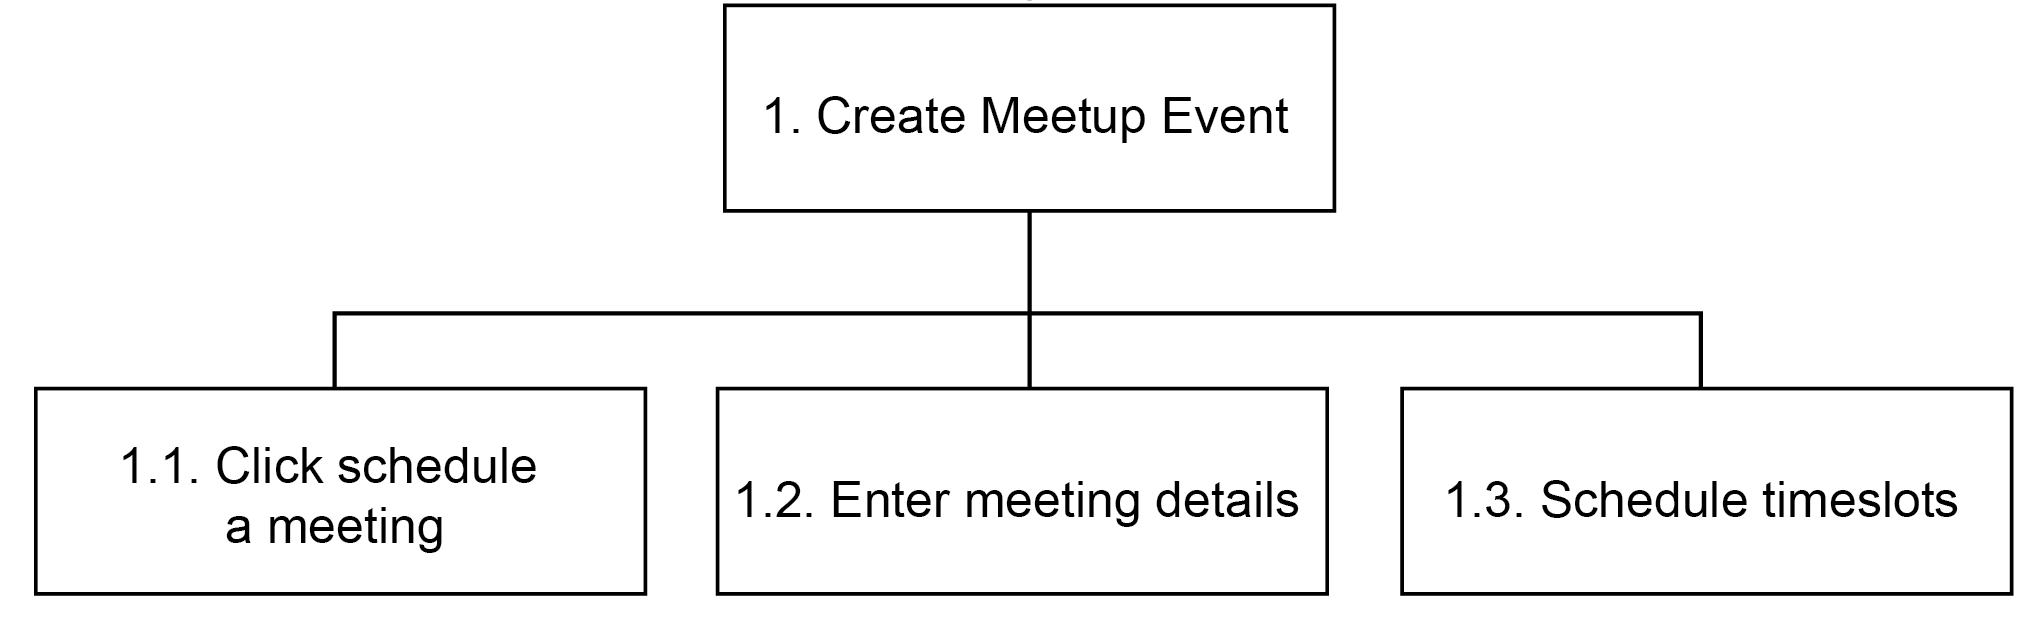
\includegraphics[width=1.75\columnwidth]{figures/NeedToMeet/HTA_host}
  \caption{\hl{Need To Meet Create Event Plan: Perform 1 by doing 1.1-1.3 in order}}
\end{figure*}

\begin{figure*}
  \centering
  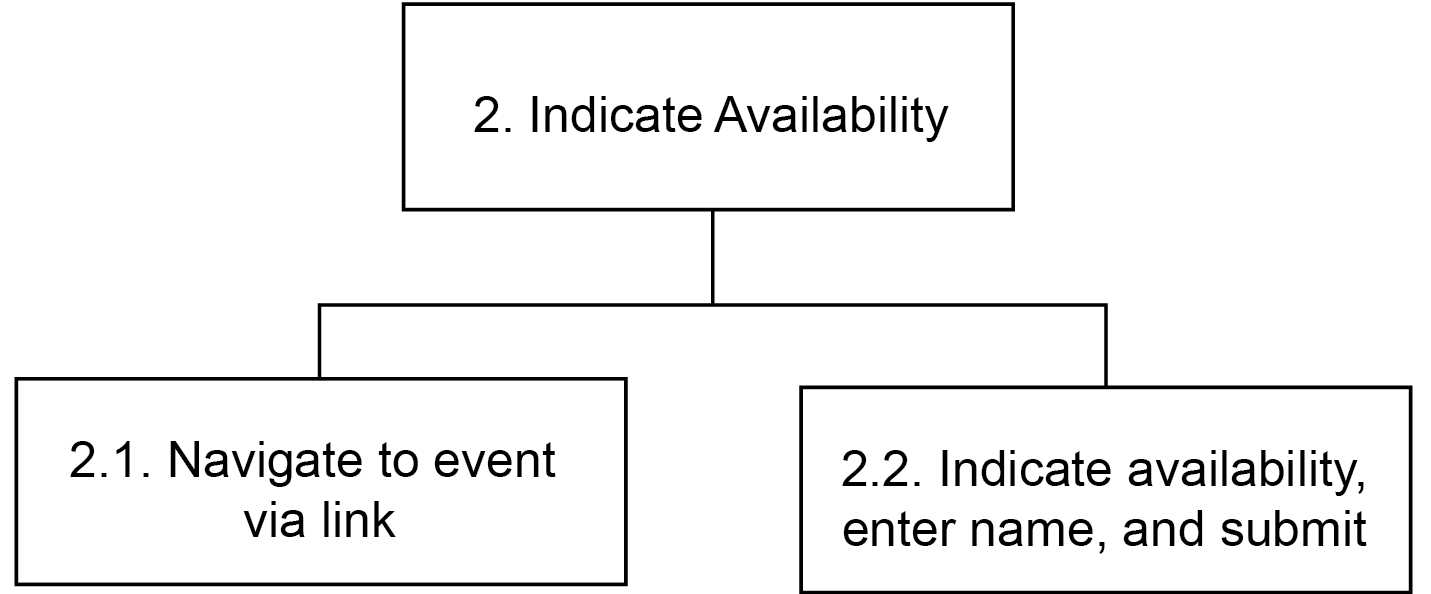
\includegraphics[width=1.75\columnwidth]{figures/NeedToMeet/HTA_attend}
  \caption{\hl{Need To Meet Indicate Availability Plan: Perform 2 by doing 2.1 then 2.2}}
\end{figure*}

\subsubsection{Critique}
"Need to Meet?" is a meeting scheduling website that helps users
enter to select mutually agreeable meeting times. Other than a noticeable 
lack of certain features (notifications of when the meeting was decided)
certain ways of interacting with the website lack discoverability, particularly
the button to open the calendar view when an attendee is selecting their available
dates and times.
\subsubsection{High Level Goals}
There are two high level goals for the website:
\begin{itemize}
	\item Creating a meeting event and showing available time slots
	\item Indicating when you can attend the meeting
\end{itemize}
\subsection{Tasks}
The major tasks users of "Need to Meet" perform include: 
\begin{enumerate}
\item Creating a Meetup Event to get availabilities of attendees
\item Click schedule a meeting
\item Enter meeting title and duration, optionally add email for correspondance
\item Using a calendar interface select the dates and times (optionally 
send people invites through the website)
\end{enumerate}
The major tasks meeting attendees need to perform are: 
\begin{enumerate}
\item Navigate to the event via the link sent by the host
\item Indicate availability, enter name, and submit
\end{enumerate}
\FloatBarrier
\subsection{Google Suite}
\FloatBarrier
\begin{figure*}
  \centering
  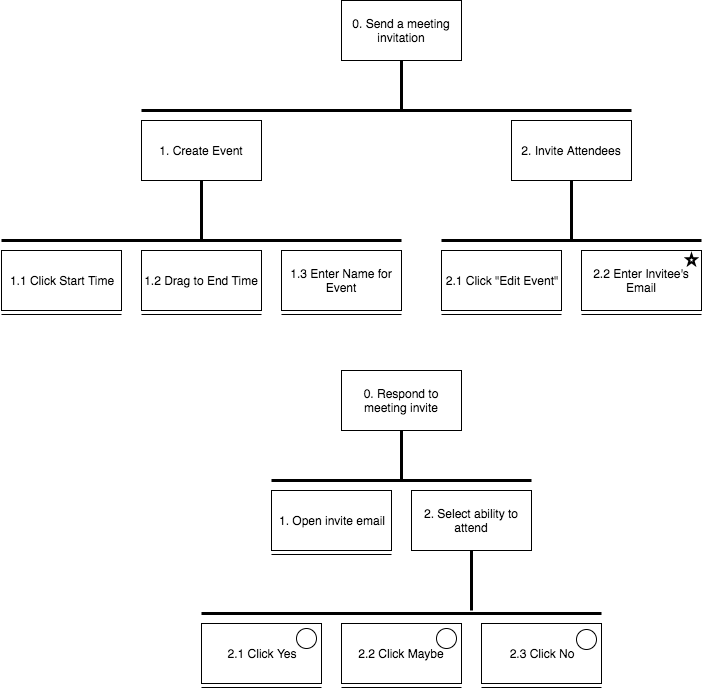
\includegraphics[width=1.75\columnwidth]{google/GoogleHTA}
  \caption{\hl{Gsuite Create Meeting Plan: Perform 1 by doing 1.1-1.3 in order, Perform 2 by doing 2.1 and repeating 2.2 for each invitee. Gsuite Respond to Invite plan: Do 1, Do 2 by doing whichever of 2.1-2.3 is appropriate}}
\end{figure*}

The Google Apps suite offer a great deal of functionality to individuals and organizations.
The tight integration of the suite offers many opportunities for improved usability.
Two such apps are Calendar and Inbox, in the tight integration for shared meeting events. 

Calendar presents the user`s schedule immediately and keeps it as the main focus of the app.
Interactions are very straightforward, and most day to day calendaring can be done without entering a menu.

Inbox is a very powerful email client focused on using email to get things done.
It has many inbox management features like snoozing emails from the inbox for some time and bundling similar low priority emails together.
It also offers quick calls to action from the inbox like event invites and flight information.

\subsubsection{Inviting Someone to a New Event with Calendar}
Users begin the invitation process by selecting or creating the event for which invitations should be sent.
This model is better than having meeting invites be a separate entity.
After creating or selecting an event, the user must enter its detail page to make invitations.
The invitees emails are entered one by one in a text field and invites are sent.
Not showing invitees from the app`s main screen is a reasonable design decision as invites are not a primary feature of Calendar

\subsubsection{Responding to a Calendar Invite from Inbox}
Calendar invites are received as regular emails which are augmented by Inbox.
When the email is opened, event details are presented and three buttons indicating ``Yes``, ``Maybe``, and ``No``.
This system is exceptionally straightforward offers little room for improvement.
One option to improve the system is to present the invited event in the context of their calendar so conflicts can be identified.
\FloatBarrier
\subsection{Outlook}
\FloatBarrier
Microsoft Outlook is an application which acts as a desktop email manager on the front. 
Outlook takes an existing email address and once added into the Microsoft Outlook registry, it allows the user to manage their emails, calenders and other various smaller actions (such as todo lists and journals). 
In addition to this, a user can use Microsoft`s servers (Microsoft Exchange Server) to allow multiple users to access shared applications (email and calender) or contact each other via Skype meeting.

To a new user, Outlook is similar to any Microsoft Office product where many of the options will be at the taskbar at the top, all categorized in their own particular category. 
This can be challenging for any users who are not familar with the Office application family, as there are many different categories that require searching. 
In addition to this, users may have a hard time knowing what each option does initially, which may cause users to be overwhelmed with the vast amount of options. 

Fortunately this is alleviated with a search function where Outlook will return results similar to what the user is looking for (e.g. searching for calender will return options regarding calender) as well each option has a brief description of what it does when it is hovered over.

Some of the few high level goals that Outlook can help a user achieve:
\begin{itemize}
	\item Date/meeting management
	\item Email management
\end{itemize}

\subsubsection{Date/Meeting Management}

\begin{figure*}
  \centering
  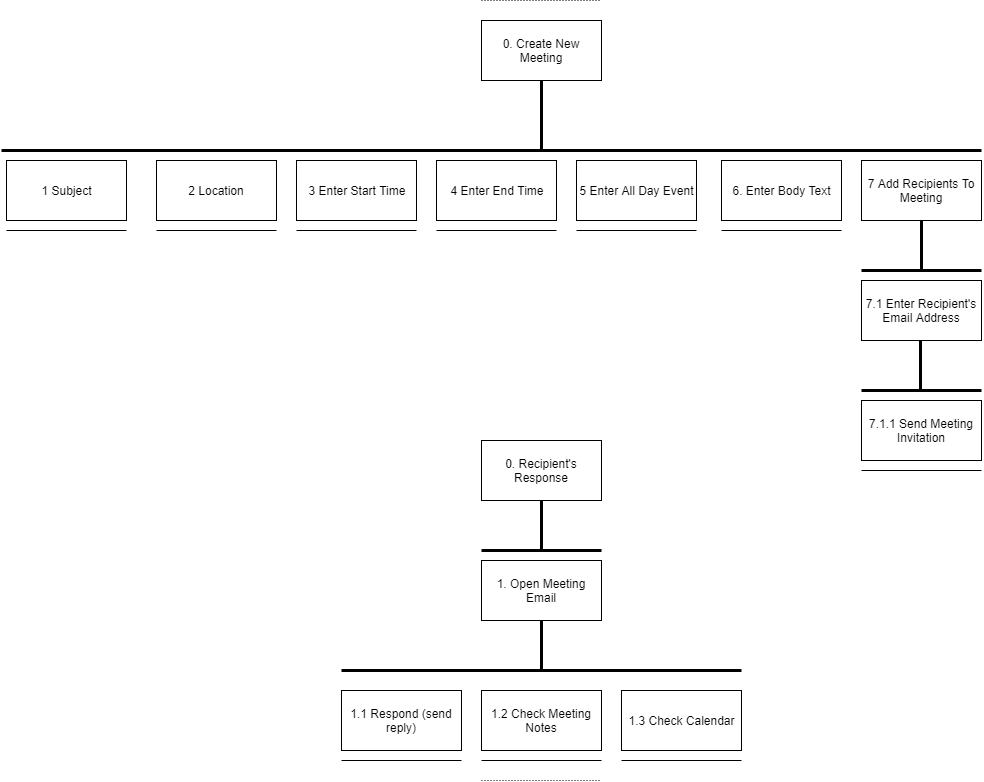
\includegraphics[width=1.75\columnwidth]{Outlook/Create_Meeting}
  \caption{\hl{Outlook Create new meeting plan: In any order Perform 1, optionally 2, 3 and 4 or 5, optionally 6, perform 7 with 7.1 for each recipient, finally 7.1.1 . Outlook Response Plan: Perform 1 and do any of 1.1-1.3}}
\end{figure*}

For date/meeting management, Outlook allows one to set up a calender between users through the Microsoft Exchange Server.
\begin{enumerate}
\item Users may create a subject
\item Users may set a location
\item Users may set a start time
\item Users may set an end time
\item Users may set the meeting as an all day event
\item Users may enter body text
\item Users will add recipients for the meeting to be sent to
\item Meeting organizer will enter all potential attending members` email address
\item Meeting will be sent to all recipients
\end{enumerate}

The date/meeting management is handled similarly to sending an email, wherein a user can use many of the features that an email already offers (e.g. creating subjects, body text, adding email recipients), as well it adds in features that help with setting up meeting details (e.g. locations and meeting times).
After the meeting details are sent, recipients will be able to respond to the notification as an email, check the calender or check meeting minutes (if meeting has occurred).


\begin{enumerate}
\item Open Meeting Email
\item Respond to email (send reply)
\item Check meeting minutes
\item Check Calendar for meeting date
\end{enumerate}

\subsubsection{Email Management}

For email management, Outlook handles users to manage both their personal email as well as a shared mailbox.  The steps can be seen through the diagram above.

\begin{enumerate}
\item Users may create a subject
\item Users may set email as a Carbon Copy (CC) to send to multiple people
\item Users may enter a body text
\item Users may check names
\item Users can select the suggested names
\item Users may attach a file/item
\item Users may add a signature
\item Users may add priority/flags to the email
\item Users will add recipients to send to
\item Users will send the email
\end{enumerate}

Outlook uses a layout that is similar to many email interfaces. It uses this interface for both personal and shared mailboxes. This allows users to navigate inside the shared mailbox or find email addresses with relative ease.
After the email is sent (via person email or within the shared mailbox), recipients will be able to respond to the email via reply.

\begin{enumerate}
\item Open email
\item Reply
\item Reply All
\item Forward
\item Forward email to new recipient
\item Archive email
\item Move email to new folder
\item Add tags to email
\item Edit the email
\end{enumerate}

For clarity, the diagram does not include a path for Reply, Reply All and Forward because it is essentially the same as the Sending Email diagram.
\FloatBarrier
\subsection{Conclusion of Analysis}

This survey has exhibited powerful applications for the organization of meetings.
The simplicity of GSuite and the time selection features of Need to Meet and Doodle offer worthwhile direction to follow.
There are clear improvements to be made by taking a close examination of the user experience flows.
We will need to take the same care in designing our product.


\section{Personas}

\subsection{Primary Persona}
\begin{itemize}
	\item \textbf{Name:} Sally Sue
	\item \textbf{Location:} Hamilton, ON
	\item \textbf{Age:} 20
	\item \textbf{Occupation:} Student At McMaster University
	\item \textbf{Tagline} ``I`ve got so got 3 midterms and 2 assignments this week and I want to be able to to go all these clubs at McMaster. I only slept 3 hours yesterday. This is fine.''
\end{itemize}

		Sally Sue is a 20 year old McMaster University student, living in Toronto, ON Canada her whole life. Throughout her life she has made it her goal to always hangout with her friends regularily and ensure that any work assigned to her is done punctually as well as with diligence. A majority of Sally`s time is spent on the computer, using all the latest web applications such as Facebook and Gmail to coordinate with friends as well as plan out her schedule for the upcoming weeks.

		When Sally had first entered into university, she began to take major interests into the surrounding student run clubs the school had to offer. She found herself not only swamped with school work but also with being in charge of some of the student clubs she joined. Despite having many tasks, she very much enjoyed the busy lifestyle she created for herself. However after repeated usage of programs similar to Outlook that caused her eyes to strain, she decided to delve into looking for alternative planning programs that could make planning more simplier and efficient as well as being able to use on the go at libraries or at home.

		Sally`s wasn`t afraid of this change, she had experienced it before when she decided to make the change from Microsoft Word to LaTeX. She initially rejected the change because of the required time to learn but discovered she much more preferred LaTeX to Word because of ability to format content much more simply. While she often learned how to use programs on her own or through simple instructions or tutorials, she discarded options that required extensive tutorials that would take much time out of her schedule to learn.

		Sally`s goals for the new programs she wanted to try were that she wanted to be able to make plans for meetings with relative ease, as well as have notifications on whether the participants have responded or not. She found that sending an email at times was not enough for some people, she also wanted to have periodic reminders for people that had not responded yet. Lastly she wanted to know who was able to attend as well as who could not and who had not responded.

		Sally had found that LetsMeet was able to meet those goals for her; she was able to send meeting invites, receive invites as well receive periodic reminders and see who was attending or not. As well, she found that LetsMeet`s options were well defined and easy to use similar to Doodle`s methodology, she found she spent little time learning how to use LetsMeet. In addition she found her eyes were not as strained as she did not spend extensive amounts of time trying to plan the meetings anymore. Sally felt her life had gotten a bit less chaotic as she spent less time sending the meeting invites and more time doing other stuff like studying or hanging out with friends. While she realized it obviously wasn`t a game changer in her schedule, it was the little victories that she cherished.

\subsection{Secondary Persona}
\begin{itemize}
	\item \textbf{Name:} Mark Muller
	\item \textbf{Location:} Frankfurt, Germany
	\item \textbf{Age:} 45 
	\item \textbf{Occupation:} Owner of Vagabund Brewery
	\item \textbf{Tagline} ``All these new technologies, they are so complicated. I just want to do my job''
\end{itemize}

Mark Muller is a 45 year old German man and proud owner of the 23 year old established and admired brewery named Vagabund Brewery. Mark`s brewery works on a 6 day basis with Sundays and holidays being closed, as well Mark is often contacted on an international basis, with a quarter of his customers being from North America. Mark`s primary language is German however he has spent enough time conducting business with clients in North America that he speaks English well enough to read and write at greater than beginner level but less than intermediate level. 

Growing up in Frankfurt, Mark had witnessed the creation of one of Europe`s most efficient underground transportation systems in Frankfurt as well as the growth of Frankfurt into a major financial hub. Mark had studied at VLB Berlin (Institute for Fermentation and Biotechnology) as well learned all his successful brewery techniques from his grandfather; with this he also learned to work hard for the days with work and rest well for the days with rest. Because of Mark`s education at VLB Berlin and his grandfather`s teachings, Mark learned at a young age to combine both the old and new techniques to make a fine tasting brew that would stand the tests of time. He was often remarked as a very intelligent man for using both the techniques; Mark often states that "We can learn from the old masters to become new masters".

Despite growing up with new technologies being introduced often, Mark could not keep up due to the high costs of technology and as such never learned extensive knowledge about them. Vagabund brewery operates with computers that from the 90s, where Mark only knows how to simply send an email on Yahoo and use Yahoo`s search engine. As well, Mark suffers from poor eyesight, looking at computer screens for more than 30 minutes causes his eyes to blur. As such, despite Mark being open to combining new techniques to create more efficient techniques, Mark is reluctant to learn about new technologies because of his disability and his minor fear of new technolgies being too complicated for him.

Mark`s close friend Karl who is often trying to introduce him to new ways to integrate him into the technological world, introduced him to LetsMeet. Karl advertised it to Mark as a way to be more efficient at planning meetings with clients as well as a way to spend less time looking at the screen. Mark had given it a try while being worried that his beginner level in computers would be his downfall. However, Mark was pleasantly surprised to find that all of LetsMeet`s options had descriptions on what they did, as well the options seemed to walk Mark through the process of planning his meeting with clients. He was simply happy with being able to plan meetings more efficiently but was even more surprised when LetsMeet updated him on when participants would respond to being able to make meetings and periodically reminded participants to respond; it was a welcome change from having to wait for a response from the client when an email was sent. The most appreciation Mark had was that the system was easy to use and he found himself spending less time looking at the screen.

Mark was estatic Karl had found him a simple and efficient system to use, it was much more informative than an email sent with the meeting information outlined. Karl also agreed to help Mark whenever he didn`t understand a function of LetsMeet; to Mark`s surprise again, he found he often did not need to call Karl for help. Overall, Mark felt much more confident to learn new technologies and was much more happier knowing that clients would receive the meeting invitations and periodic reminders to respond; he would be able to worry less about meetings not being received or information being missed on an email from his Yahoo account.

\subsection{Secondary Persona}
\begin{itemize}
	\item \textbf{Name:} Lori Vaudry
	\item \textbf{Location:} Toronto, Ontario
	\item \textbf{Age:} 59
	\item \textbf{Occupation:} Early Retiree (Was an HR/Operations Executive)
	\item \textbf{Tagline} ``We`re both so busy but we definitely should do lunch sometime!''
\end{itemize}

Lori grew up in Montreal and learned both English and French, but her English was much stronger because that`s what she spoke at home
She earned an MBA at McMaster and moved to Toronto once both of her kids were born, but they`ve since moved out to university. 
In Toronto she worked her way up to an executive job at CIBC.
At the bank she became skilled with the main path of tools she used regularly outlook expert.
She wouldn`t typically play with software and preferred to learn from written instructions.
Her goto way to schedule events was a back and forth of outlook calendar invites; 
and since Lori was an executive people would generally move other commitments to fit her schedule.
 
Lori was offered a substantial retirement package from the bank and decided to accept the change and retire. 
Since then she`s picked up a number of new activities.
She`s got the energy and physical ability to play tennis and the manual dexterity to play piano.
Scheduling group events like book club with the other busy ladies in her social circle was difficult and her son suggested she try Let`s Meet after using it at University.
She`s nervous it might be too complicated for her friends who aren`t computer people at all, but it sounds like it would be really useful to keep organized.

Sitting at her kitchen island with her son nearby incase she needs help, Lori opens her MacBook and goes to Lets Meet.
She needs to schedule next week`s book club at a time that works for everyone.
The last few meetings were scheduled carelessly and some people had to miss them.
Opening the web page she just enters the information it asks for, and never has to guess what to do.
She invites most of the members by email but makes sure to invite Jackie with her phone number because Jackie doesn`t check her email often.

In three days Lori`s gotten responses from the whole club, even Jackie.
It looks like 7 PM  on Tuesday works for everybody, so she confirms the date, and the whole club is notified.
The whole experience was way easier than a back and forth with everyone about their availability, and being able to push the date to everyone was really handy

\section{Usability Evaluation}

\subsection{Pre-Test Questionnaire}

For the Pre-Test Questionnaire, we had opted for these questions:

\begin{itemize}
	\item You are experienced with meetings
	\item You schedule meetings often
	\item Some of the current meeting scheduling apps are tedious to use
	\item You find your meeting invites are ignored by invitees	
\end{itemize}

these questions were answered in Likert scale format with 5 possible answers: Strongly Disagree, Disagree, Neutral, Agree, and Strongly Agree. These questions were more so to gather if the user had experience with using other meeting scheduling apps and to determine their level of meeting knowledge (e.g. do they attend meetings often, do they notice at the meetings that many invitees do not read/receive their invite).

\subsection{Test Cases}
\begin{enumerate}
\item Create a Meetup Event and input the information
\item Schedule the meeting by using the calender interface to select dates and times to send the meeting
\item Navigate through the invite and indicate name and availability
\end{enumerate}

For test case 1, we will test the user's ability to create the event. The user will be tasked to create an event (Meetup Event), wherein they will click the option to create a meetup event and input all the meeting information (e.g. meeting details). The user will be tested on their ability to complete a meeting scheduling, we will test if the user is able to complete the meeting scheduling relatively fast, if the instructions are easy to follow we can see whether the instructions are relatively easy to follow. Test case 2 is within test-case 1.

For test case 2, we will test the user's ability to schedule the time for the meeting. The user will be tasked to schedule the meeting by using the calender interface to select dates and times for the meeting. The users will be tested on how well they use the calender features are, this is tested through how many mistakes they make while trying to select the date or selecting the time the meeting will take place (The users know which days and time they will select prior to selecting). We can determine how simple or easy the calender feature is to use based on how many mistakes the user made, if the user made multiple select/deselect of the dates or readjustments to the meeting time.

For test case 3, we will test the user's ability to respond the meeting invitation. The user will be tasked with responding to the meeting through the RSVP feature, wherein they will click on the RSVP feature and respond to it. In addition to this. We will be testing the relative ease the user has to responding, whether they understand the instructions or find them complicated.

\subsection{Post-Test Questionnaire}

For the Post-Testing Questionnaire, we had opted for these questions:
\begin{itemize}
	\item LetsMeet had a simple to use interface
	\item The Create Event and inputing the information was easy to use
	\item Scheduling a meeting with the calender interface was easy to follow and input
	\item Responding to meeting invites was simple and easy
	\item The View Results of RSVP was helpful and easy to follow
	\item LetsMeet was a satisfying experience to use (e.g. easy to use or hard to use, would use again)
	\item Compared to other apps, using LetsMeet was an easier experience
\end{itemize}

All questions from the post-testing questionnaire were asked with a Likert scale model with the questions having 5 possible answers: Strongly Disagree, Disagree, Neutral, Agree, and Strongly Agree.

As well we have included some more written type questions to be able to gauge more specific problems that users had. This way we can see whether potential design problems are more so user preference or if they shared amongst the users
\begin{itemize}
	\item Which aspects of LetsMeet did you find difficult to use
	\item Which aspects of LetsMeet did you find easy to use?
	\item Which aspects of LetsMeet did you like?
	\item Which aspects of LetsMeet did you dislike?
	\item What would you change about this app?
\end{itemize}

The point of both these types of questions were to gauge which areas may have potential design problems, if there was an average agreement on which areas were not done well or were not simple for the user to use. For example, if our post-test questionnaire had many users answering with disagree to a feature done well, we know that they have some problem with it. The written answers may be able to help us understand which particular area they find is difficult or that they do not like to use.

What is our evaluation evaluating?
\begin{itemize}
	\item How simple is our app to use. Are they able to quickly create a meeting? As well is it simple/easy to create the meetings? A more quick meeting scheduling for a new user can mean that the user is able to understand the instructions well and complete the given task.

	\item As well our we are evaluating if it is a satisfying experience, how satisfied are our users in using the app? Do they get frustrated when adjusting some of the informations (e.g. readjusting the time for scheduling meetings).

	\item What are some critical flaws in our design, what are some ideas that we have had about our implementation that may have been redundant or done better. What are some of the areas that our users feel are not easy to use or find better versions in already existing applications.
\end{itemize}

\section{Results}

For Pre-Testing Questionnaire, this was the result:

The first question asked was if "You are experienced with meetings". The results of that question came to 1 user responding with neutral, 3 users responding with agree and 1 user responding with strongly agree.

The second question asked was if "You schedule meetings often". The results of that question came to 2 users responding with disagree, 1 user responding with neutral, 1 user responding with agree, and 1 user responding with strongly agree.

The third question asked was if "Some of the current meeting scheduling apps are tedious to use". The results of that question came to 2 users responding with disagree, 2 responding with neutral and 1 user responding with agree.

The fourth question asked was if "You find your meeting invites are ignored by invitees". The results of that question came to 1 user responding with neutral, 2 user responding with agree, and 2 user responding with strongly agree.

For Post-Testing Questionnaire, this was the result:

The first question asked was if "LetsMeet had a simple to use interface". The results of that question came to 3 users responding with neutral and 2 responding with agree.

The second question asked was if "The Create Event and inputing the information was easy to use". The results of that question came to all 5 users answering with agree.

The third question asked was if "Scheduling a meeting with the calender interface was easy to follow and input". The results of that question came to 3 users answering with neutral and 2 users answering with agree.

The fourth question asked was if "Responding to meeting invites was simple and easy". The results of that question came to 3 users answering with agree and 2 users answering with neutral responses.

The fifth question asked was if "The View Results of RSVP was helpful and easy to follow". The results of that were all 5 users answering with agree.

The sixth question asked was if "LetsMeet was a satisfying experience to use (e.g. easy to use or hard to use, would use again)". The results of this question were 4 users answered the question with neutral and 1 user answered the question with agree.

The seventh question asked was if "Compared to other apps, using LetsMeet was an easier experience". The result of this were that 1 user answered with disagree, 2 users answered with neutral and the last 2 users answered with agree.

As for the written answers, we noticed that the users found the calendar system to be easy to use and likable but the military time (24 hour format) used for selecting the time was disliked and not an easy feature to use. This had affected their vote for the third question; if the 24 hour format was changed to 12 hour format, they would most likely change their answer to agree.

\section{Discussion}

Based on our questionnaires and written answer responses, we have found that some of our features are not as simple to use as we had initially thought. A common reoccurring issue that users had was the method to select the time for the calendar. Users found that the slider was slightly less convenient to use than traditionally inputting the number, users found it may be easier to input the time as a unit than to keep readjusting the slider on each side to get the correct meeting time. However the main issue that users had with the slider was that the time was displayed in military time (24 hour format). This was a main issue for users because it was odd for them to try to convert the 24 hour format to 12 hour format while having to keep readjusting the slider; all users reported that they usually schedule hangouts with friends or keep track of time with the 12 hour format. Another issue that users had in our testing was having to re-input invitee's emails over and over again. This is not an issue if a user only has to use the application once in a while but when they use the app regularly, having to manually input the email addresses every time a new event is to be schedule can become very tedious especially if there are always 3 invitees per event. Users stated that if we had implemented some sort of system to store invitee's information (e.g. having an account) or if the way to send the invite was more simplistic (e.g. doodle's send meeting link feature), this could be negated.

What went right in our design was the calendar system (not including the time slider). All the users had agreed that the calendar feature was easy to use, the users had responded positively to the ability to click on the dates in calendar format. Users had found it was nice to see the days their events were planned on as a day on the calendar instead of just an option, as well it was simplistic and easy to use as they just had to click on the date to set the event to that date rather than input the information manually. Another feature that went right in our design was the View Results feature. Users liked the ability to see which invitees could not attend or which invitees have not responded yet. A problem from our users that we found from the pre-testing questionnaire was that most of the users had some problems with invitees not receiving or responding to the invite. The users found the View Results of RSVP feature to be a very simple and effective way to check whether or not invitees have received or responded to the invite.

What went wrong with our design was the 24 hour format usage in the time slider for the calendar feature. As mentioned earlier in issues, the majority of users had expressed that they almost always use 12 hour format and while they are familiar with 24 hour format, they are not used to trying to set a time in 24 hour formatting; making it difficult for them to use.

In subsequent iterations of the program, some aspects of the design we would look to modify would be the 24 hour formatting for the time slider and the ability to store invitee's email addresses or having some sort of way to create saved invitee lists. The 24 hour formatting was not well received with our users and we aim to make the LetsMeet very simple and efficient for the user; users should spend more time planning what day their event will be and what time it will be rather than trying to convert an unfamiliar time format to a familiar time format. The ability to store invitee's emails or save lists would be a feature that should be implemented in future updates. The original idea was for users to be able to have a simple way to schedule a meeting. As the application is used more often, users should have new features that will help keep the usage of the app simple. The ability to save invitee's emails to use as a quick reference for later meetings would greatly increase efficiency for the user, as they would not have to waste time and manually input email addresses of regular invites.

\section{Conclusion}

Overall, our app LetsMeet was designed to be a simple and efficient way for users to create events, schedule them and also check on the status of invitees on whether they had received or responded to the invite. We had create this app with the features mentioned above with the ability to schedule meetings via clicking on a date on the calendar and viewing the results of the invitees' RSVP. We had found that while we had some design features that worked very well with our goal, we also had some features that were not as simple as we thought it would be when we implemented it. Some of the features that worked well for the user were the calendar feature and view results of RSVP; simultaneously a feature of the calendar that did not work well was the 24 hour formatting for the calendar's time slider. 



\FloatBarrier


\balance{}

% BALANCE COLUMNS
\newpage

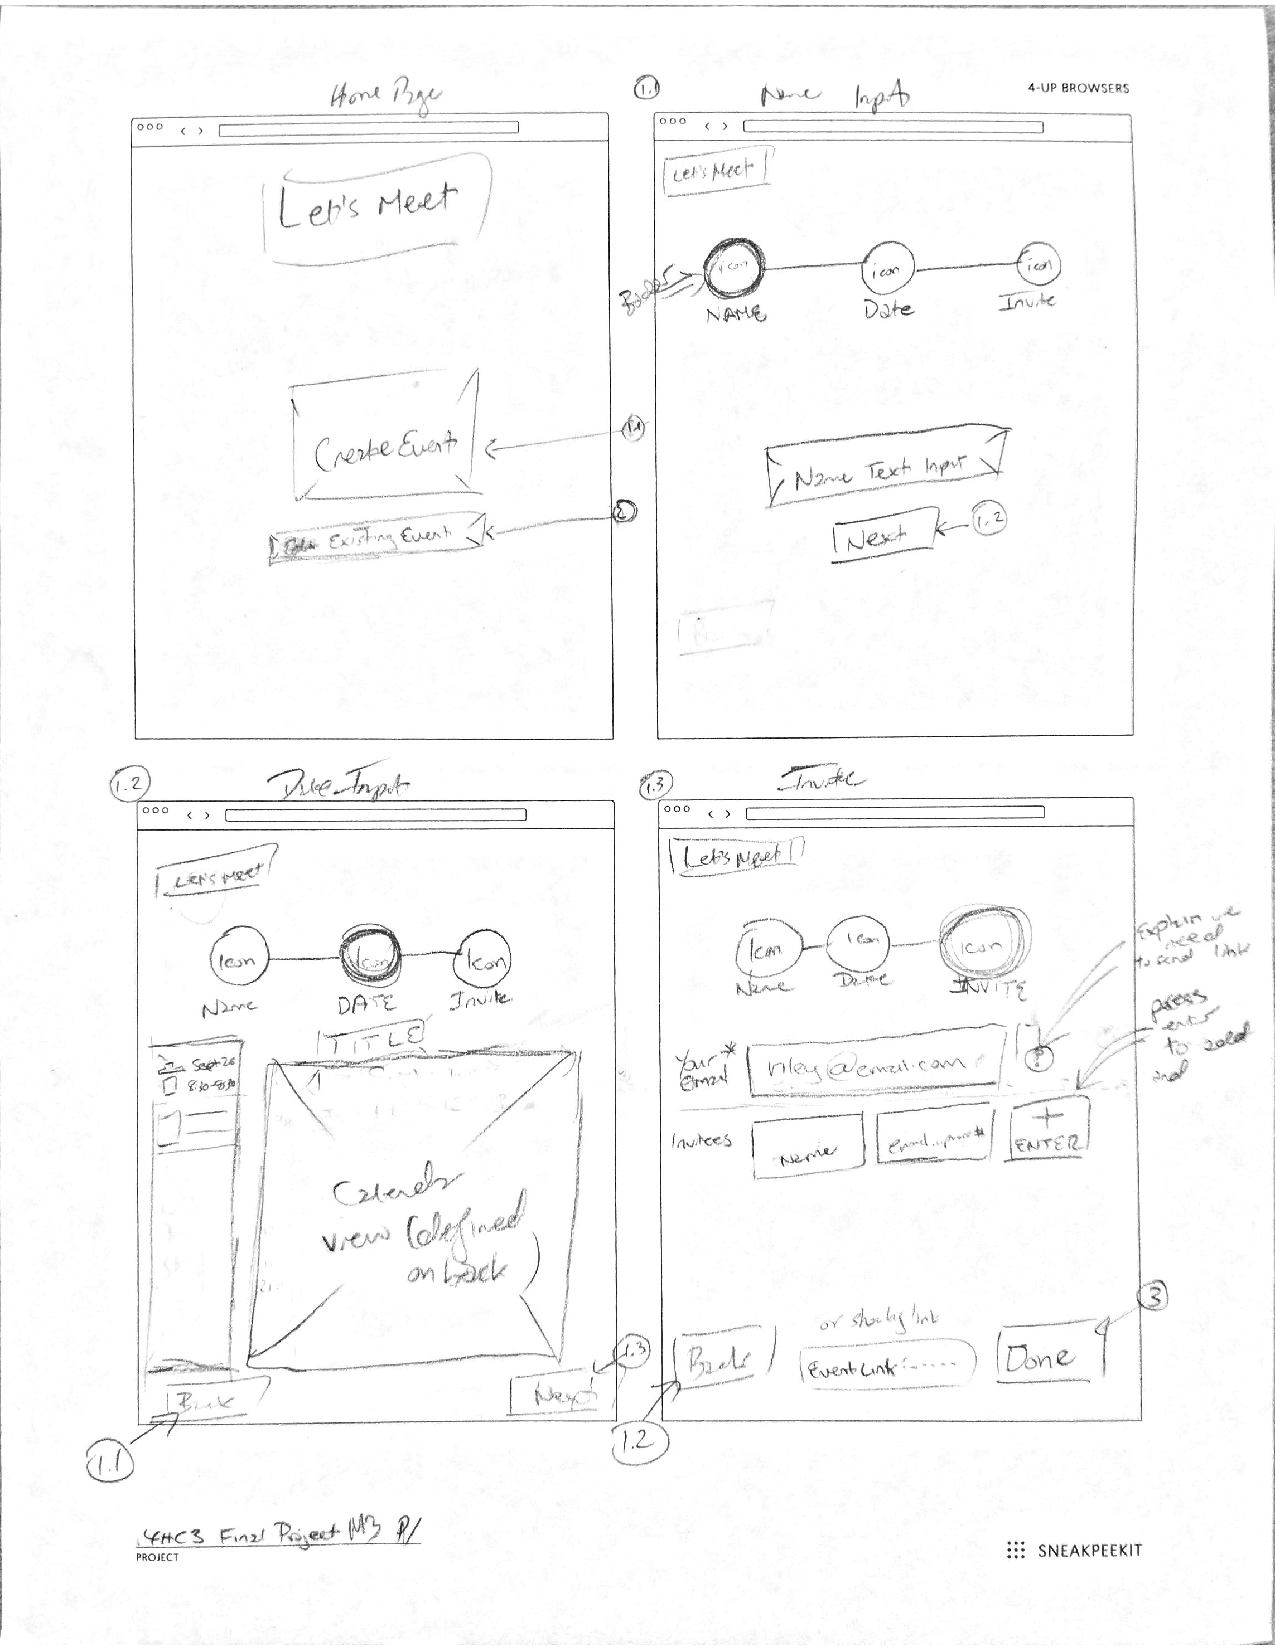
\includepdf[pages=-,width=\textwidth]{LetsMeetSketches.pdf}


\section{UI Design}
\subsection{Proposed UI HTA}

\FloatBarrier
\begin{figure*}
  \centering
  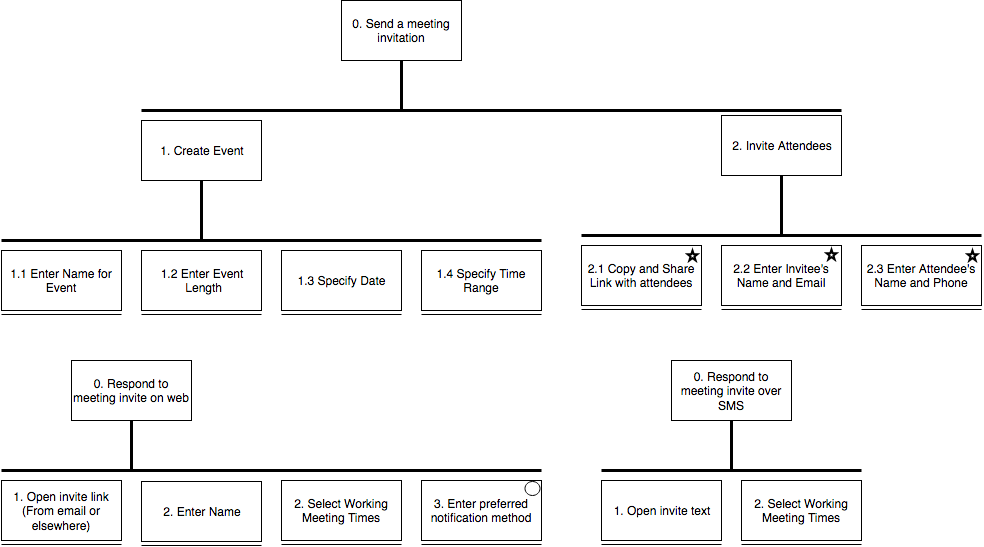
\includegraphics[width=1.75\columnwidth]{figures/LetsMeetHTA}
  \caption{Let's Meet invite plan: Perform 1 by doing 1.1, 1.2 and repeating 1.3 and 1.4 for each date of availability, Doing 2 by doing 2.1-2.3 as many times as there are participants to be invited by that method. Let's Meet Response on web plan: perform 1-3 in order and optionally 4 if necessary. Let's Meet Response on SMS plan: Do 1, then 2}
\end{figure*}
\FloatBarrier

\subsection{High Fidelity Mockup}

\subsubsection{Event Creation Flow}
\begin{figure*}
  \centering
  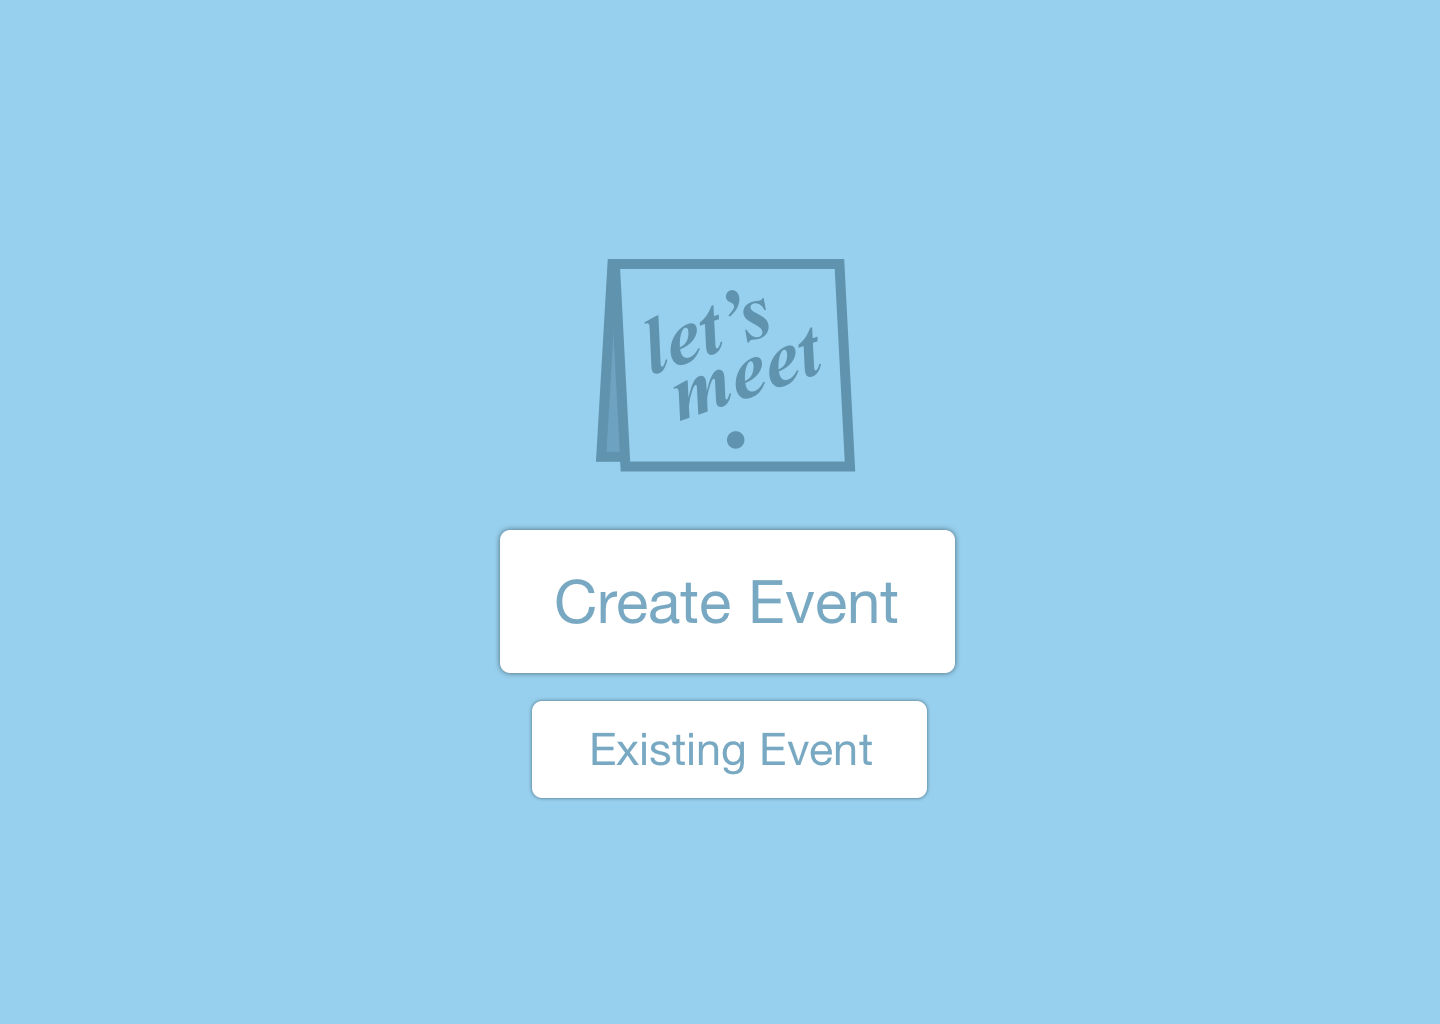
\includegraphics[width=1.75\columnwidth]{Mockup/Home}
  \caption{Current homepage}
\end{figure*}

\begin{figure*}
  \centering
  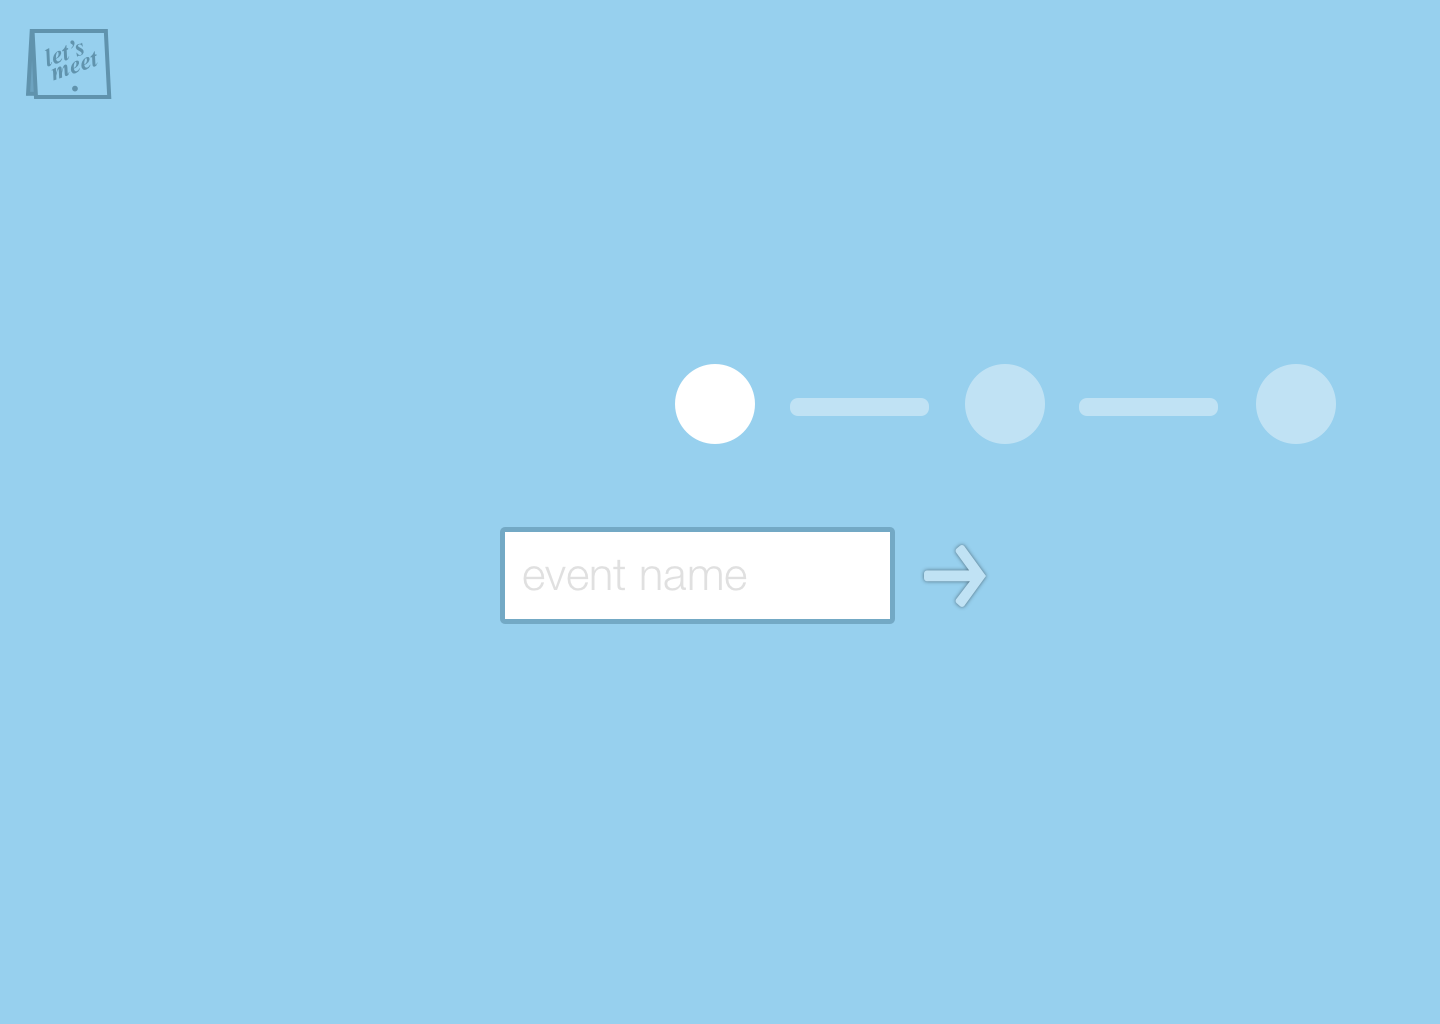
\includegraphics[width=1.75\columnwidth]{Mockup/EventName}
  \caption{Current event name entry}
\end{figure*}

\begin{figure*}
  \centering
  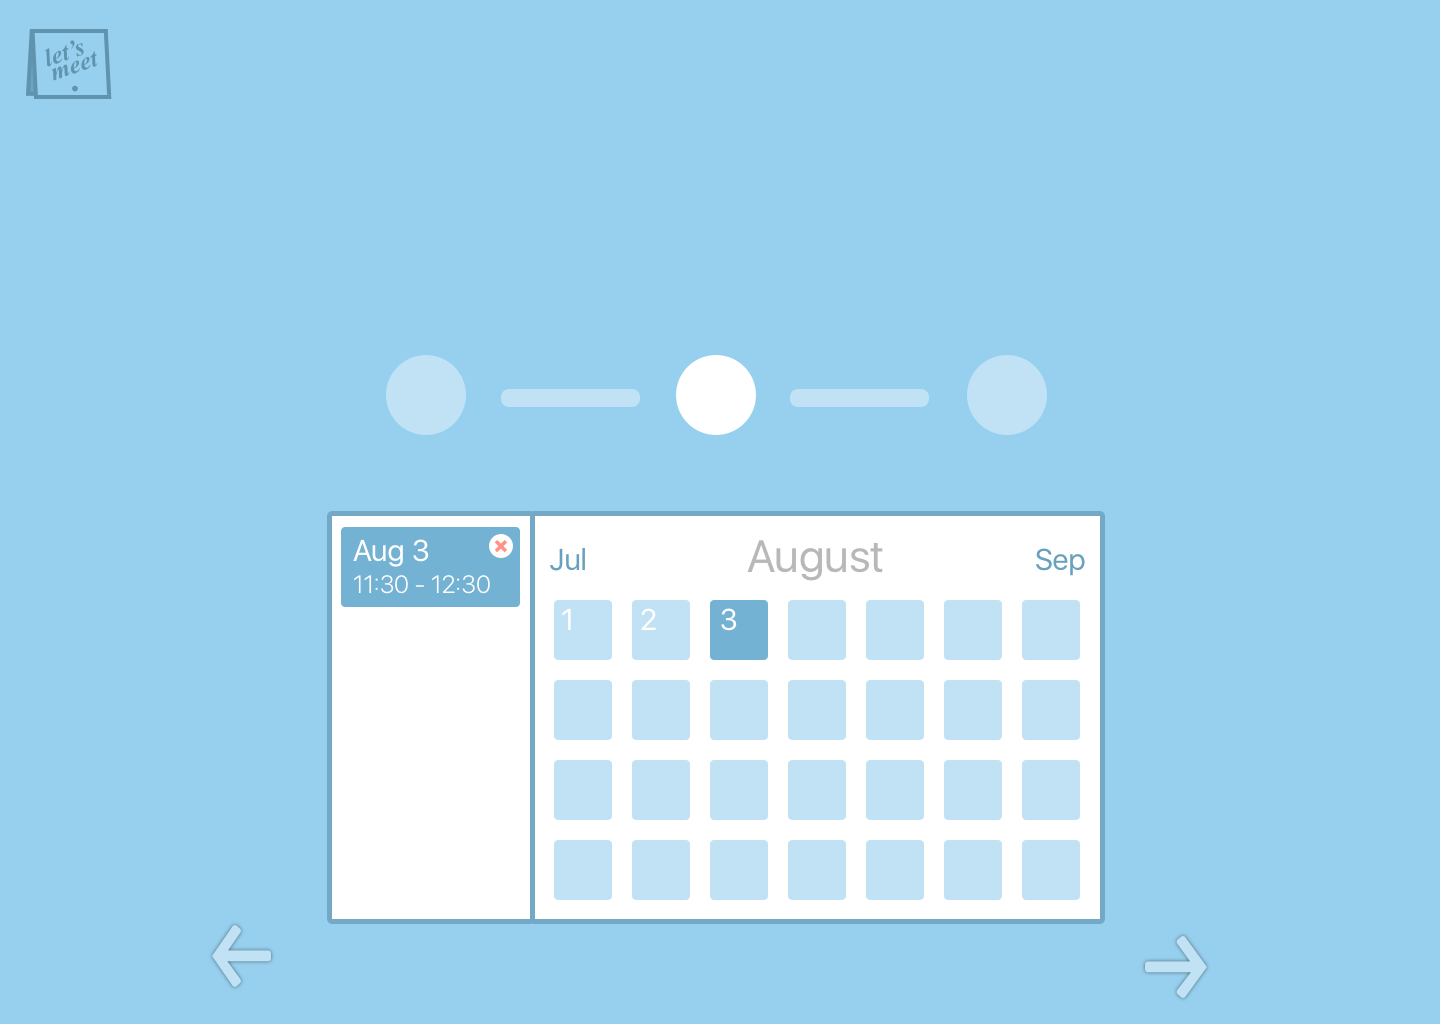
\includegraphics[width=1.75\columnwidth]{Mockup/DateSelection}
  \caption{Current event date selection}
\end{figure*}

\begin{figure*}
  \centering
  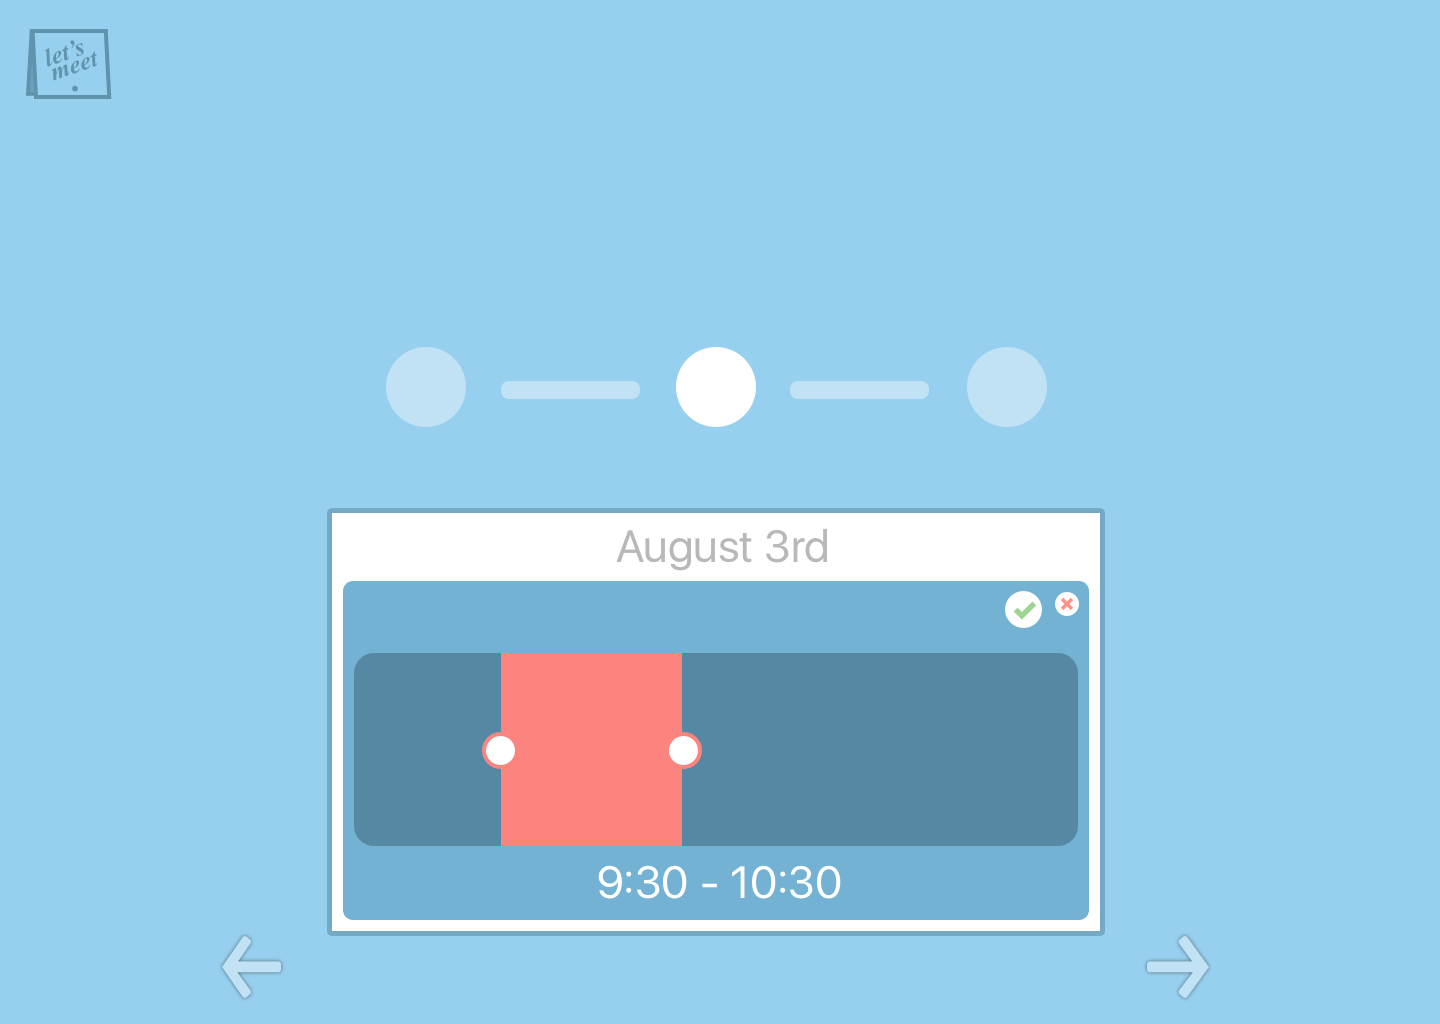
\includegraphics[width=1.75\columnwidth]{Mockup/TimeSelection}
  \caption{Current event date selection}
\end{figure*}

\begin{figure*}
  \centering
  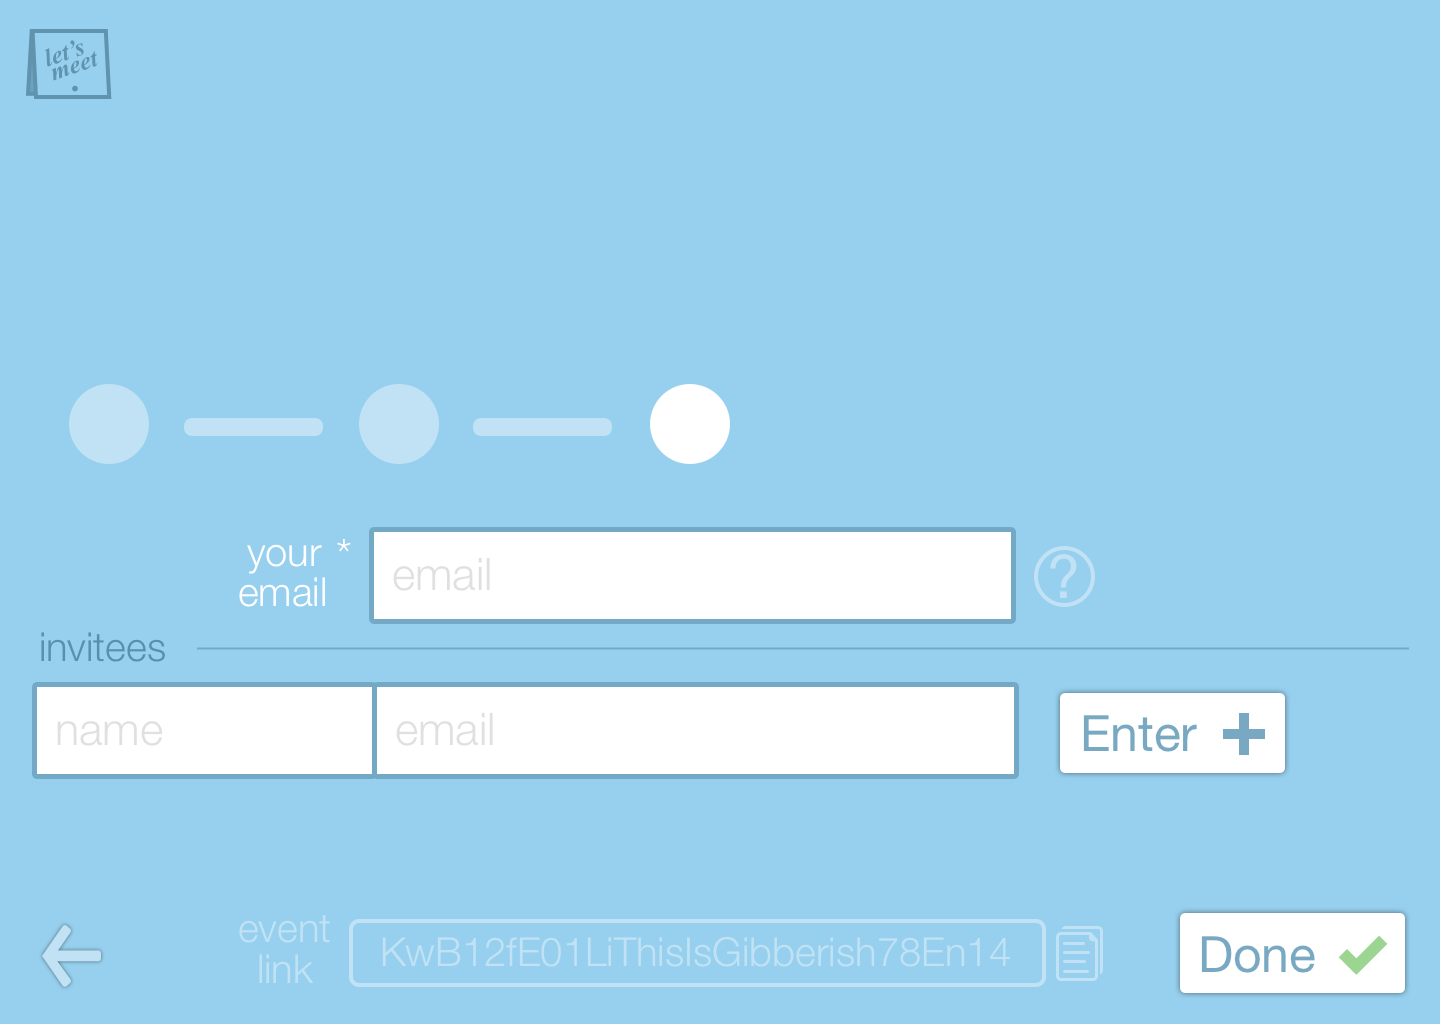
\includegraphics[width=1.75\columnwidth]{Mockup/Invitees}
  \caption{Current event invitation screen}
\end{figure*}
\FloatBarrier

\subsubsection{Event Responses}

\begin{figure*}
  \centering
  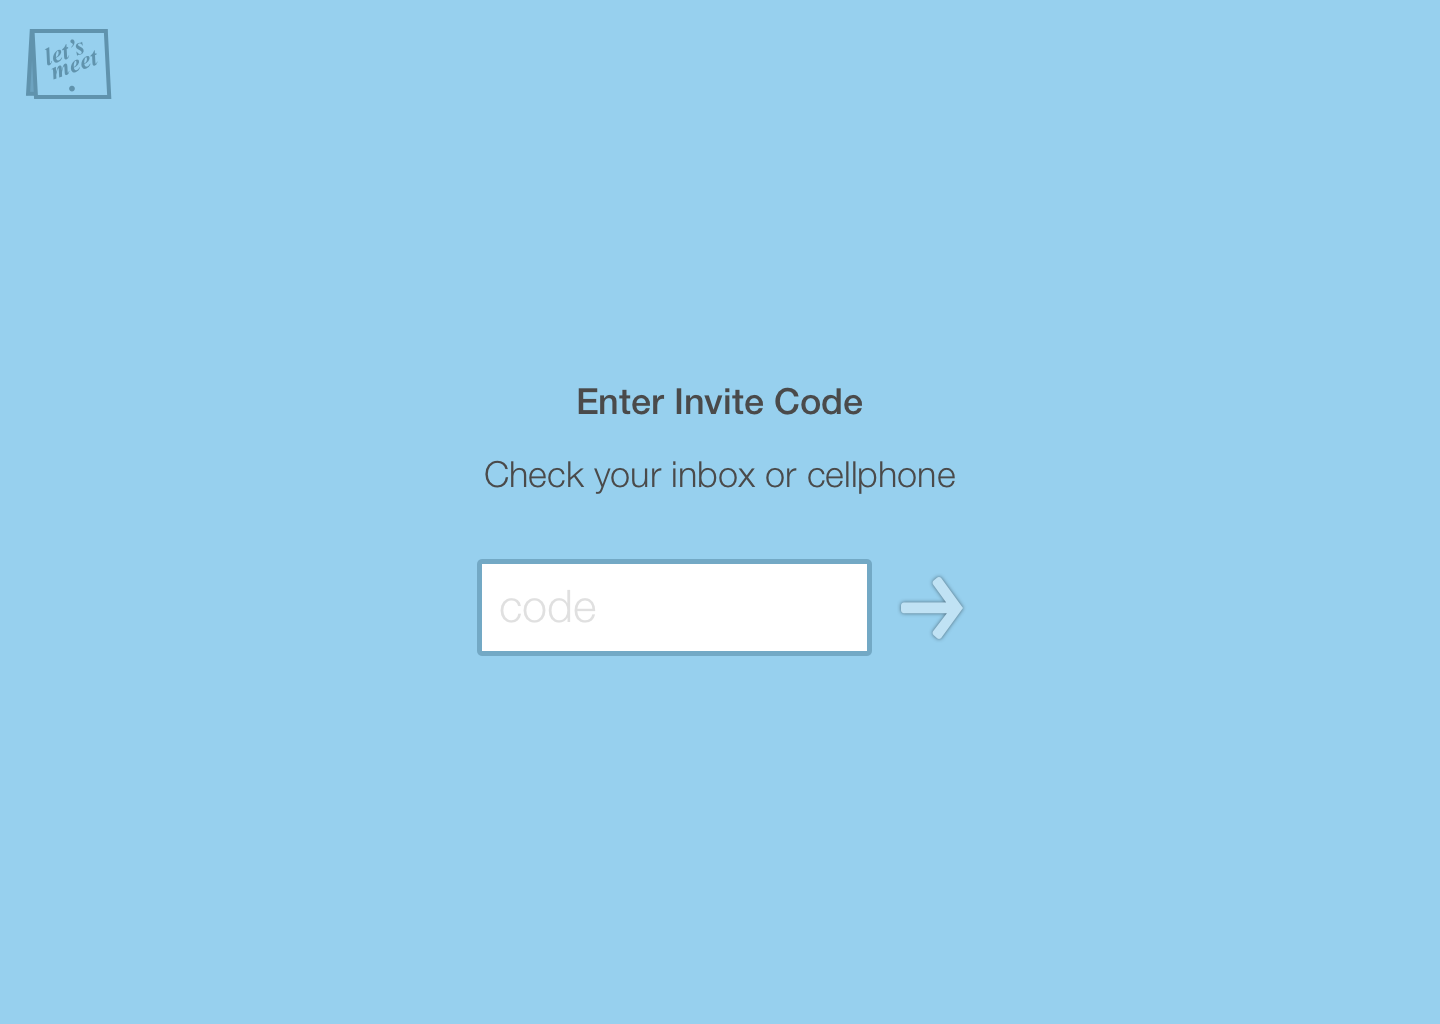
\includegraphics[width=1.75\columnwidth]{Mockup/EnterEventCode}
  \caption{Current Optional event code entry for non conventional entry users. Email and Link Clickers will not see this dialogue}
\end{figure*}

\begin{figure*}
  \centering
  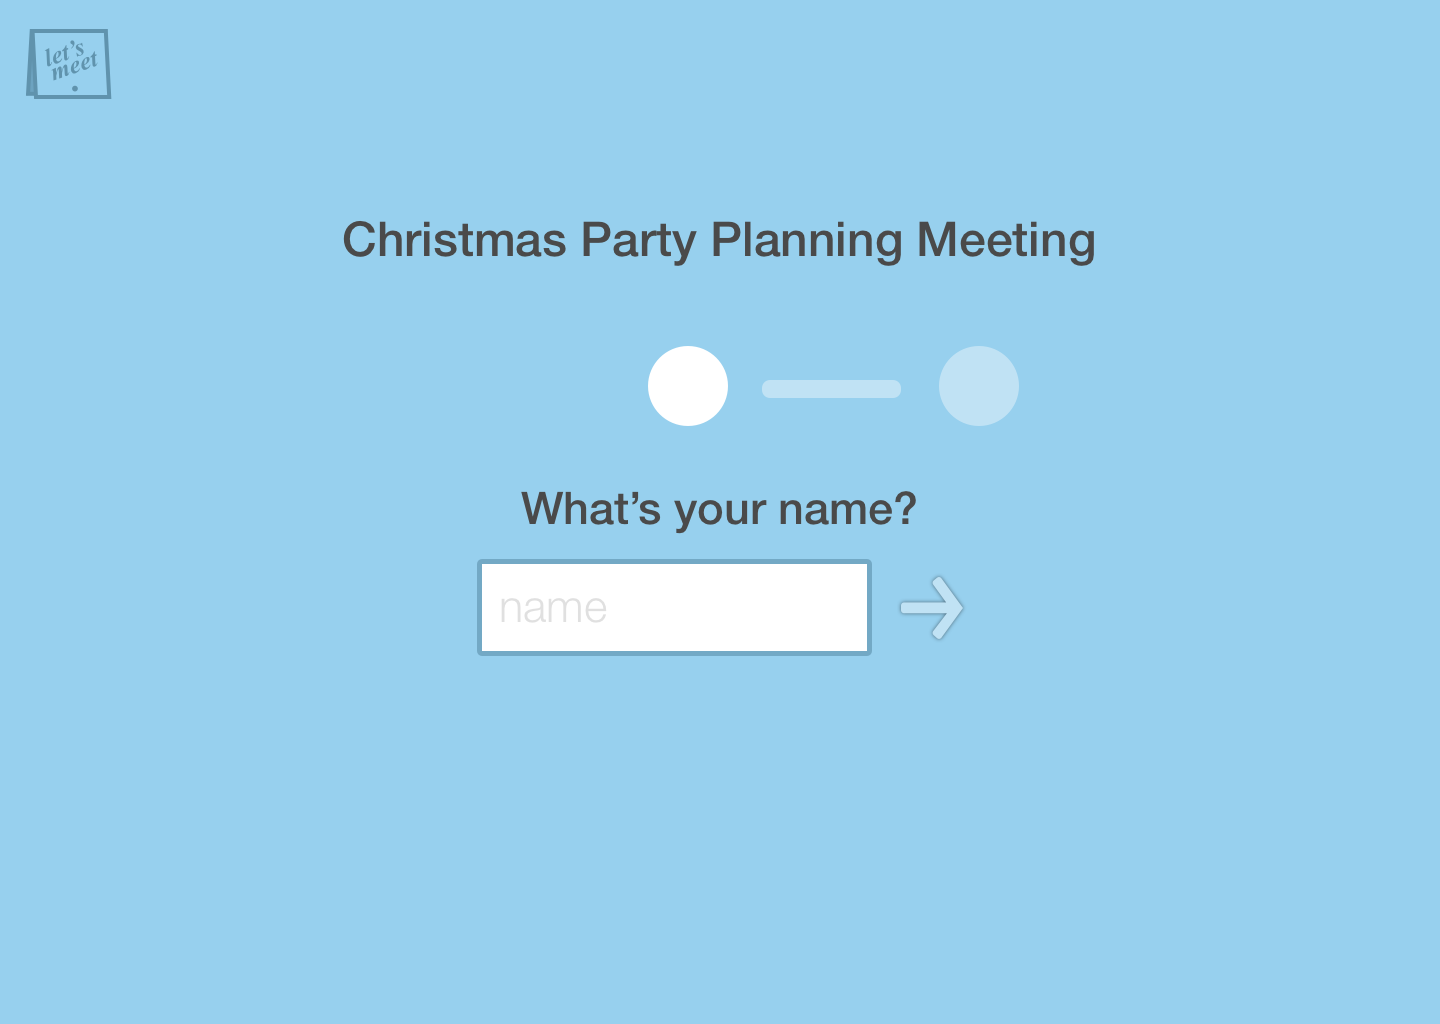
\includegraphics[width=1.75\columnwidth]{Mockup/RSVPEnterName}
  \caption{Current RSVP name entry}
\end{figure*}

\begin{figure*}
  \centering
  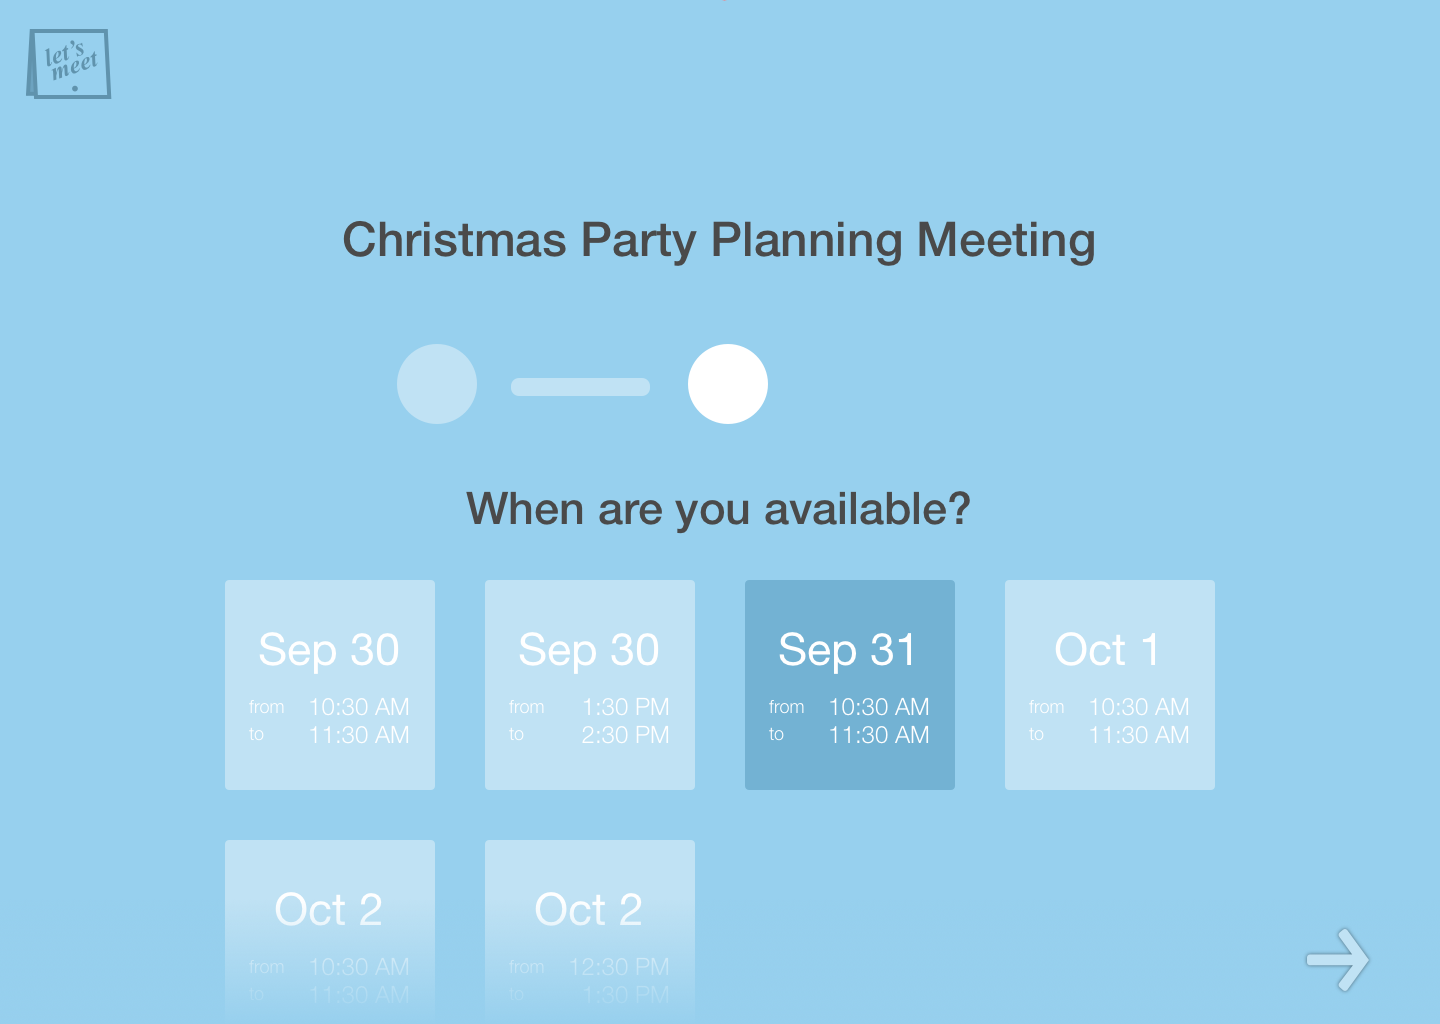
\includegraphics[width=1.75\columnwidth]{Mockup/RSVPEnterAvailability}
  \caption{Current RSVP availability entry}
\end{figure*}

\begin{figure*}
  \centering
  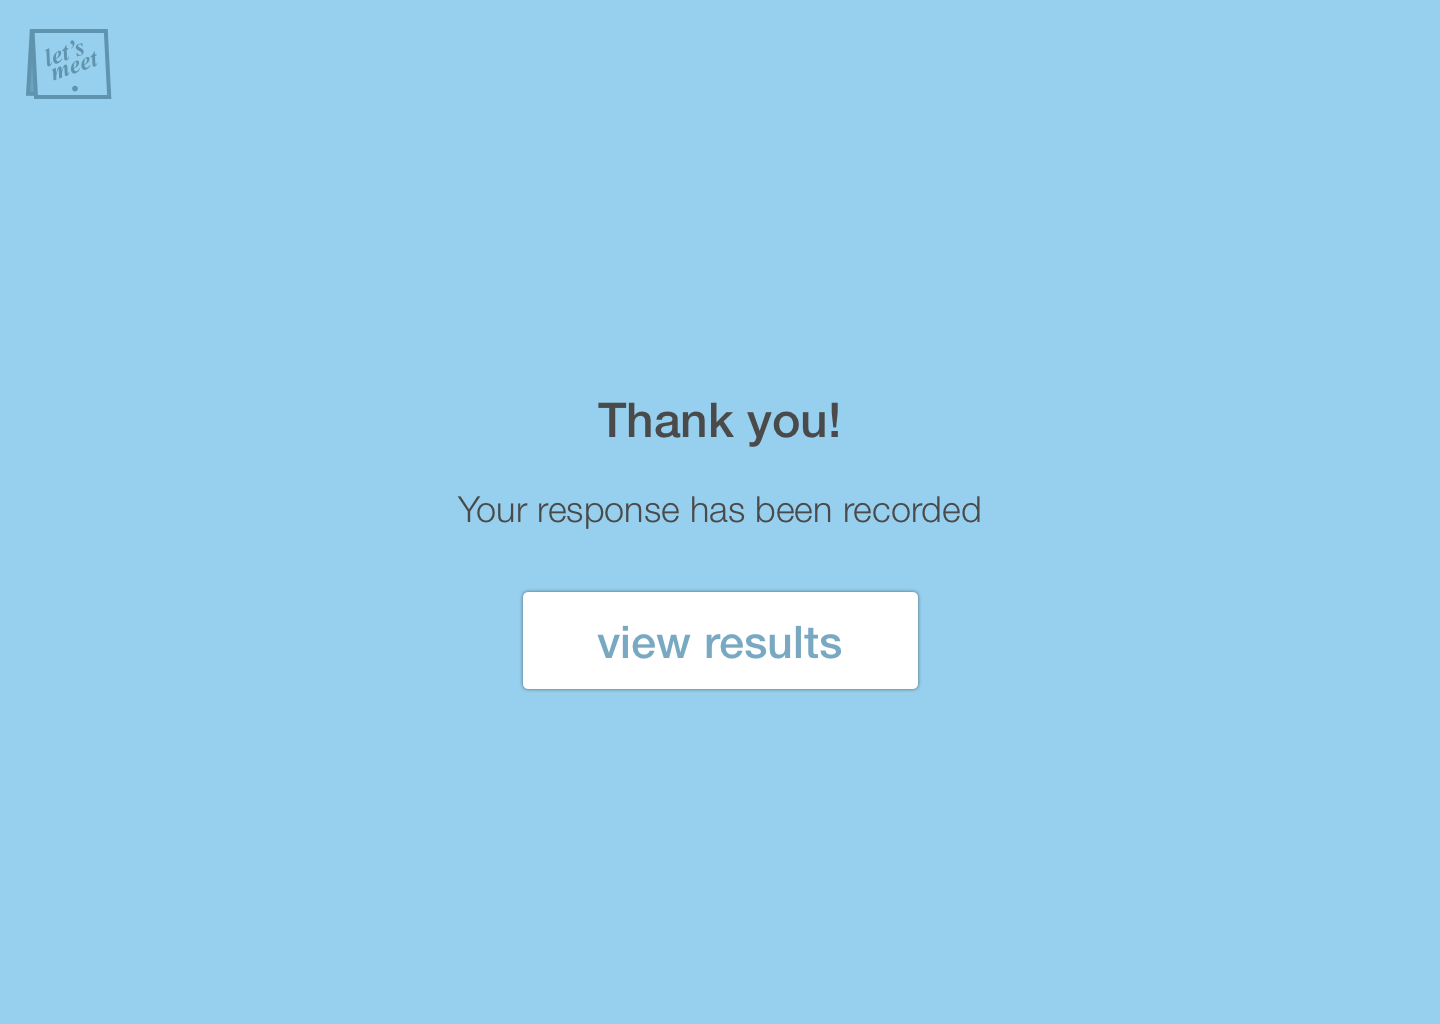
\includegraphics[width=1.75\columnwidth]{Mockup/RSVPResponse}
  \caption{Current end screen after RSVP entry}
\end{figure*}
\FloatBarrier

\begin{figure*}
  \centering
  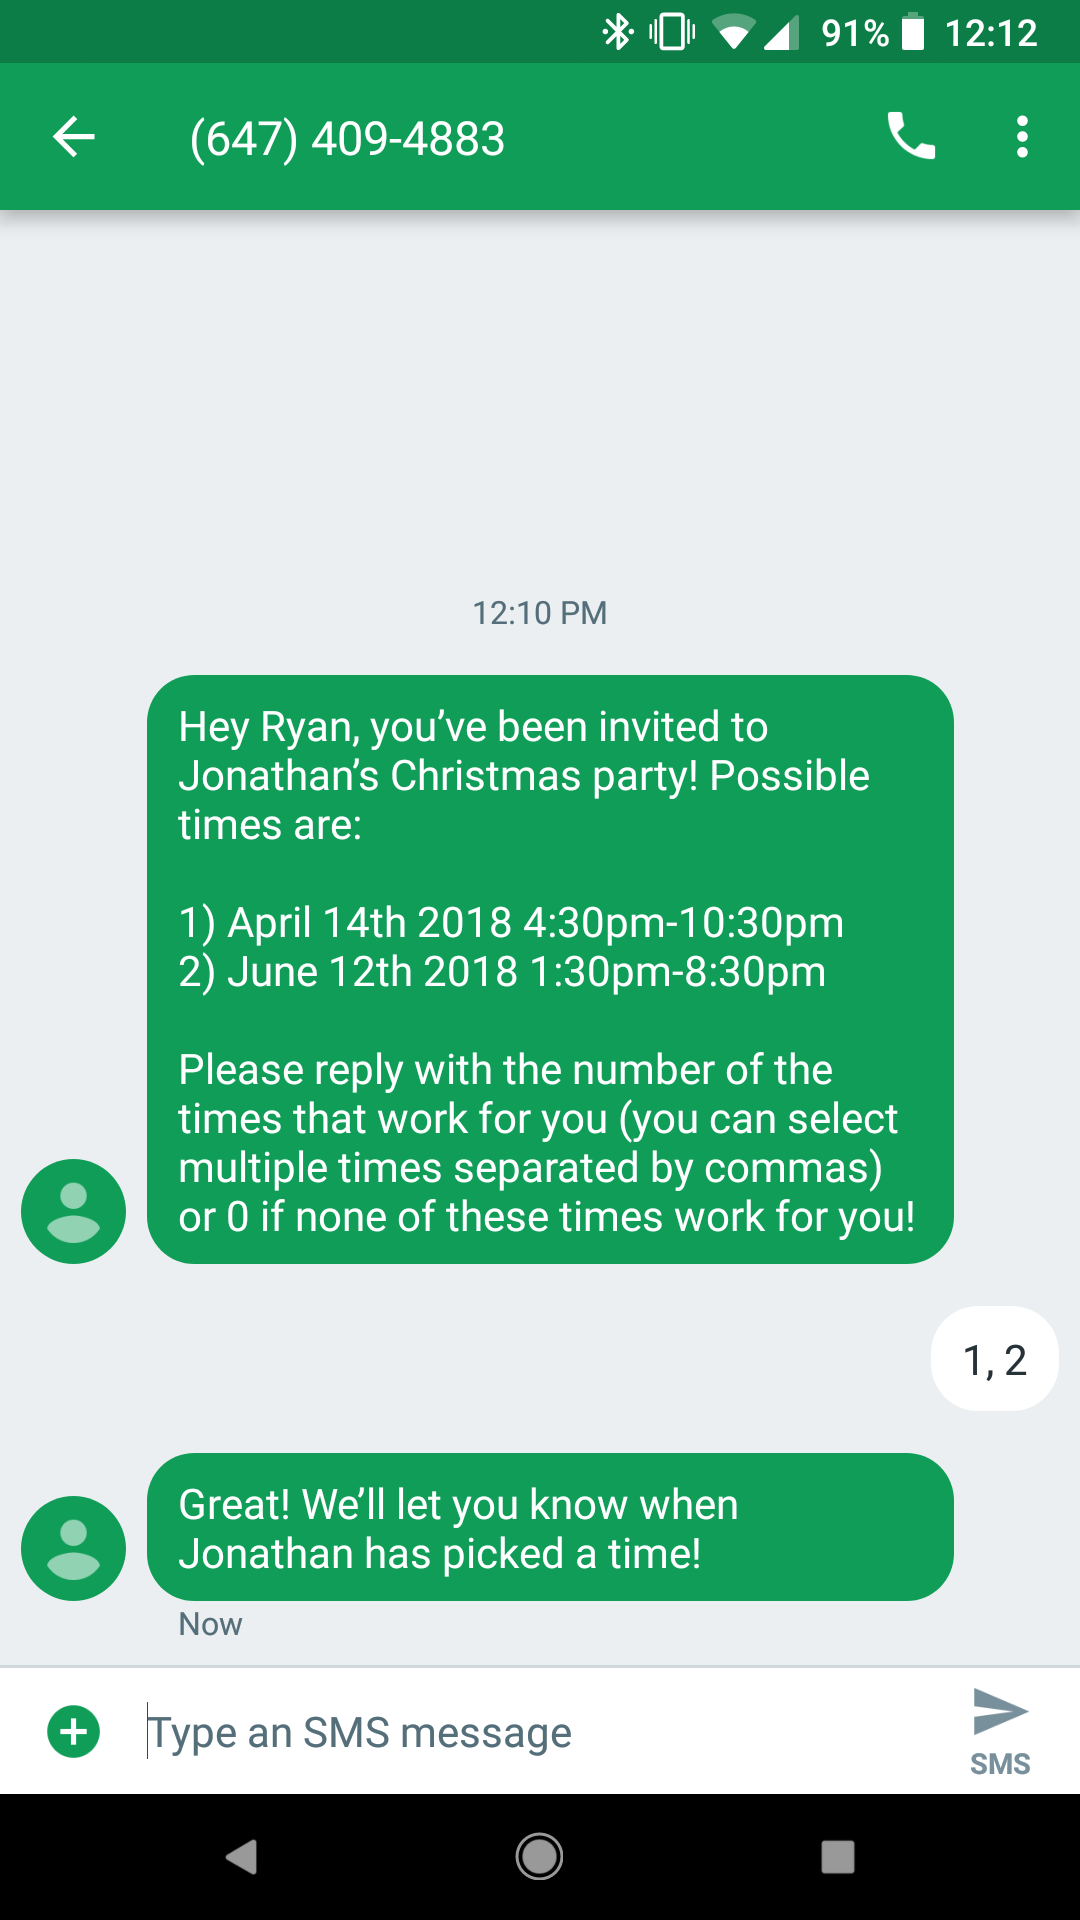
\includegraphics[width=1.3\columnwidth]{Mockup/TextResponse}
  \caption{Current text invite response flow}
\end{figure*}
\FloatBarrier

\subsubsection{Event Time Selection}

\begin{figure*}
  \centering
  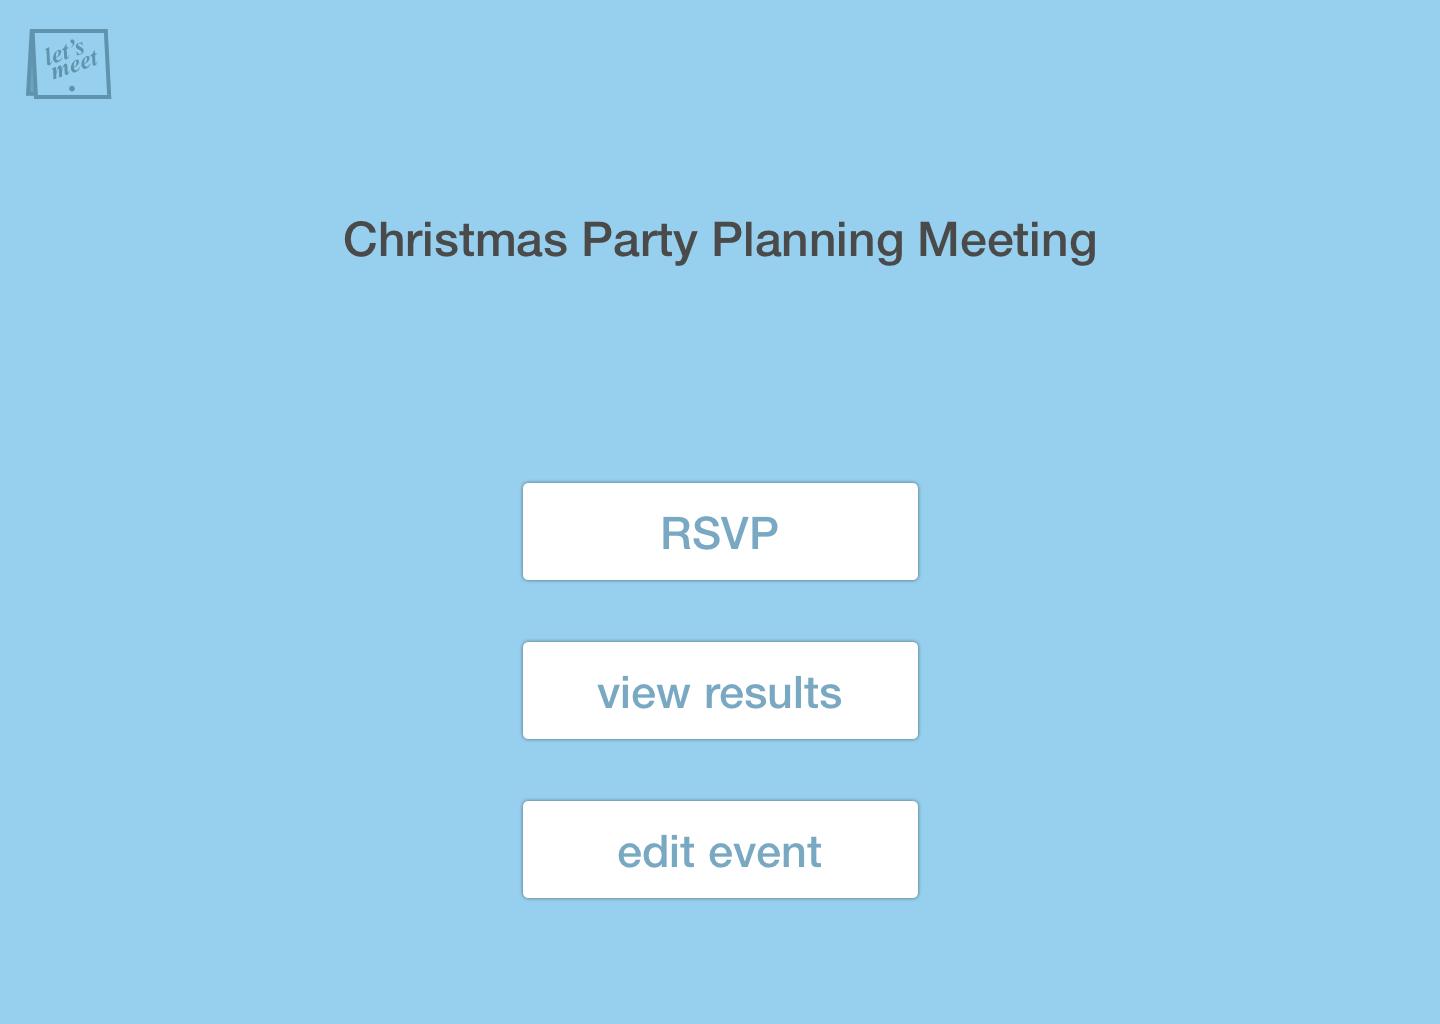
\includegraphics[width=1.75\columnwidth]{Mockup/Options}
  \caption{Current Host options screen}
\end{figure*}

\begin{figure*}
  \centering
  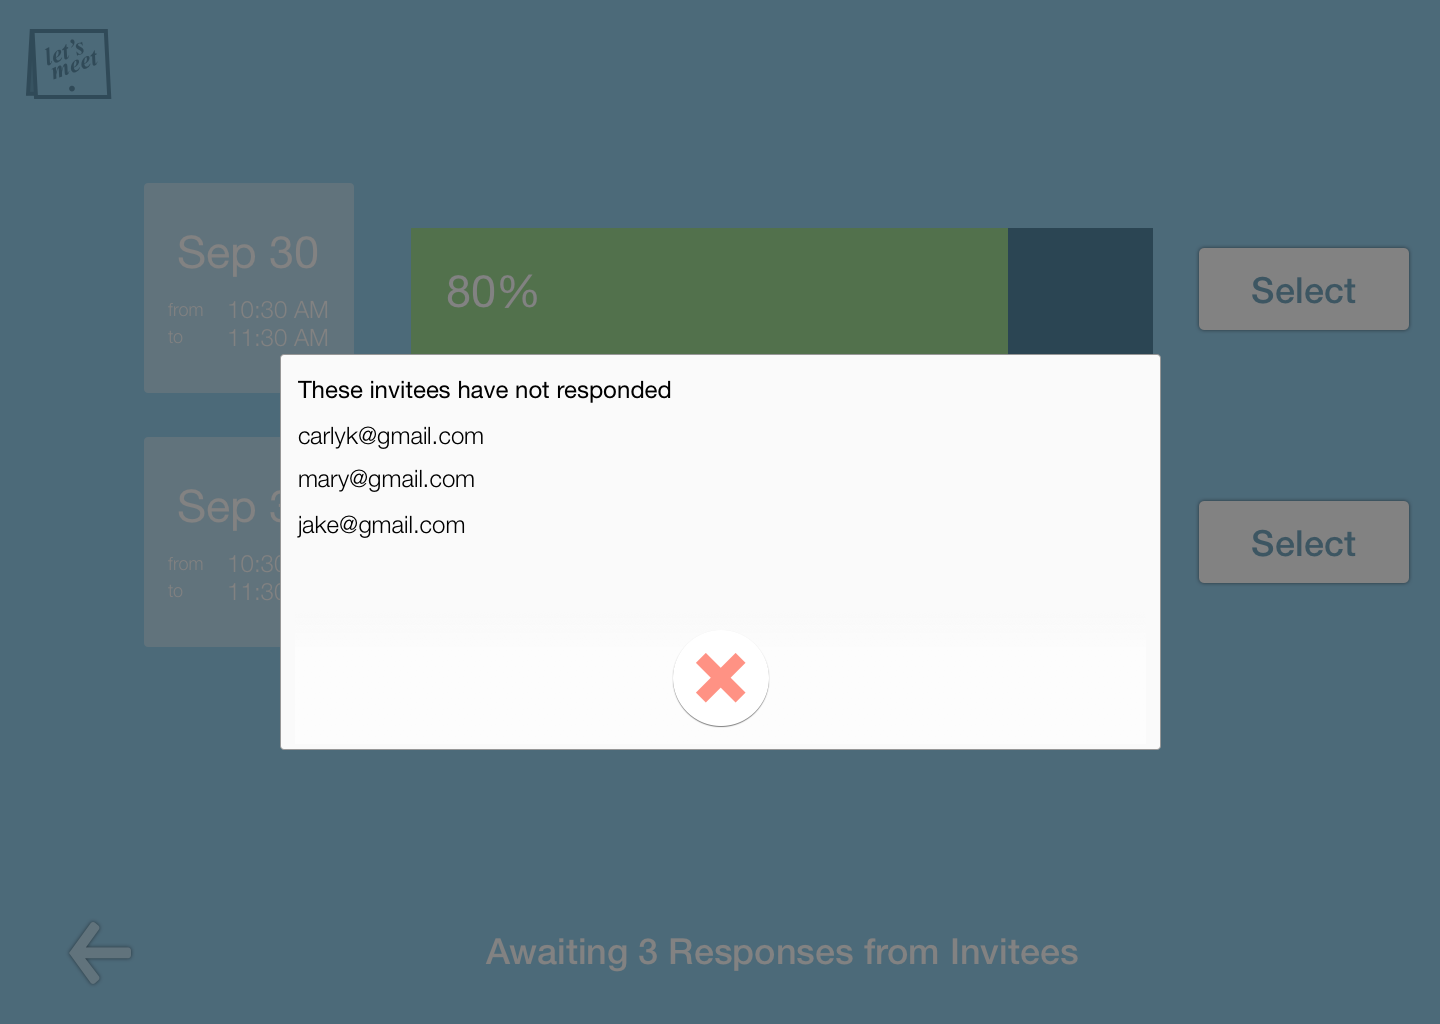
\includegraphics[width=1.75\columnwidth]{Mockup/ResultsInviteesDialog}
  \caption{Current Host invitee response dialog}
\end{figure*}

\begin{figure*}
  \centering
  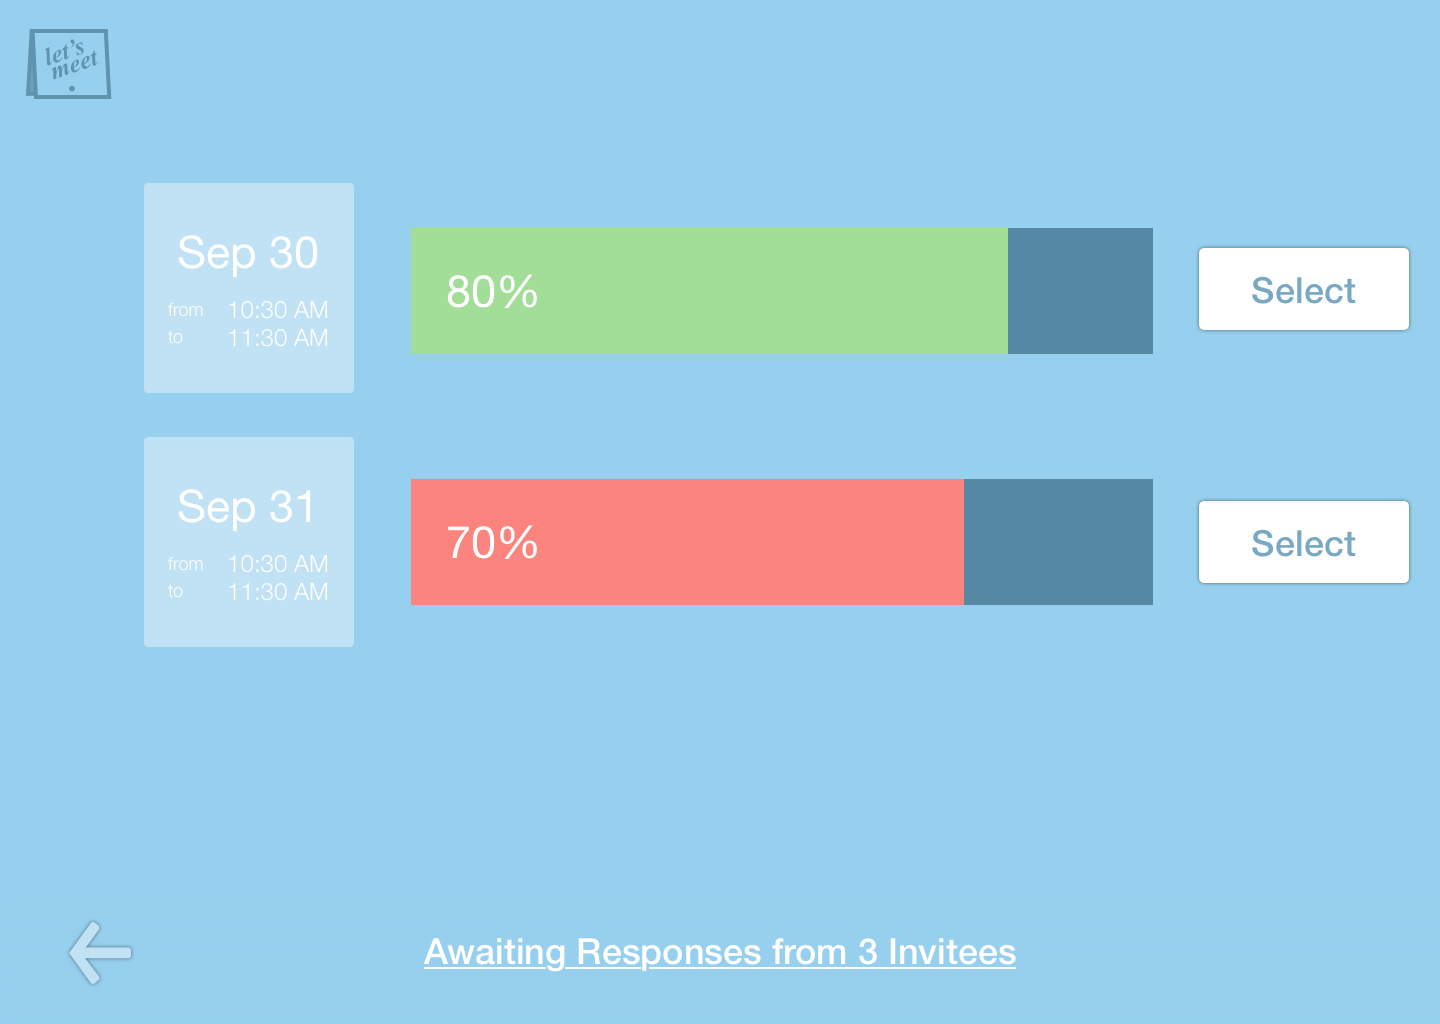
\includegraphics[width=1.75\columnwidth]{Mockup/Results}
  \caption{Current Results page}
\end{figure*}

\begin{figure*}
  \centering
  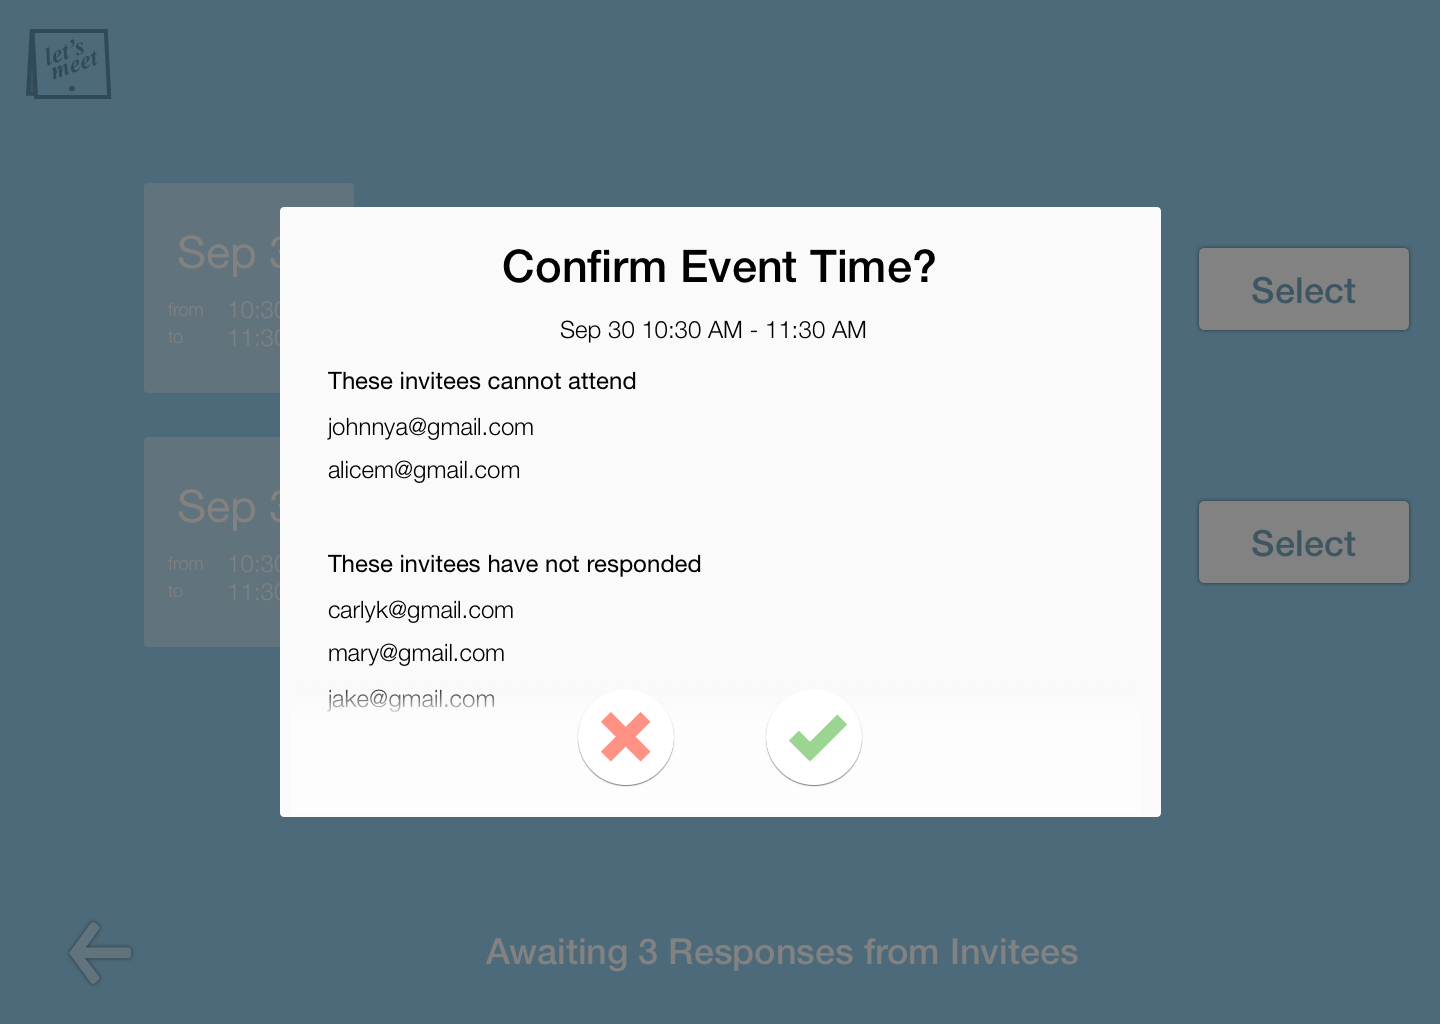
\includegraphics[width=1.75\columnwidth]{Mockup/ResultsSelectDialog}
  \caption{Current Host time confirmation dialog}
\end{figure*}
\FloatBarrier

\balance{}
\newpage

% REFERENCES FORMAT
% References must be the same font size as other body text.
\bibliographystyle{SIGCHI-Reference-Format}
\bibliography{sample}

\section{Appendix}

\begin{figure}[H]
\centering
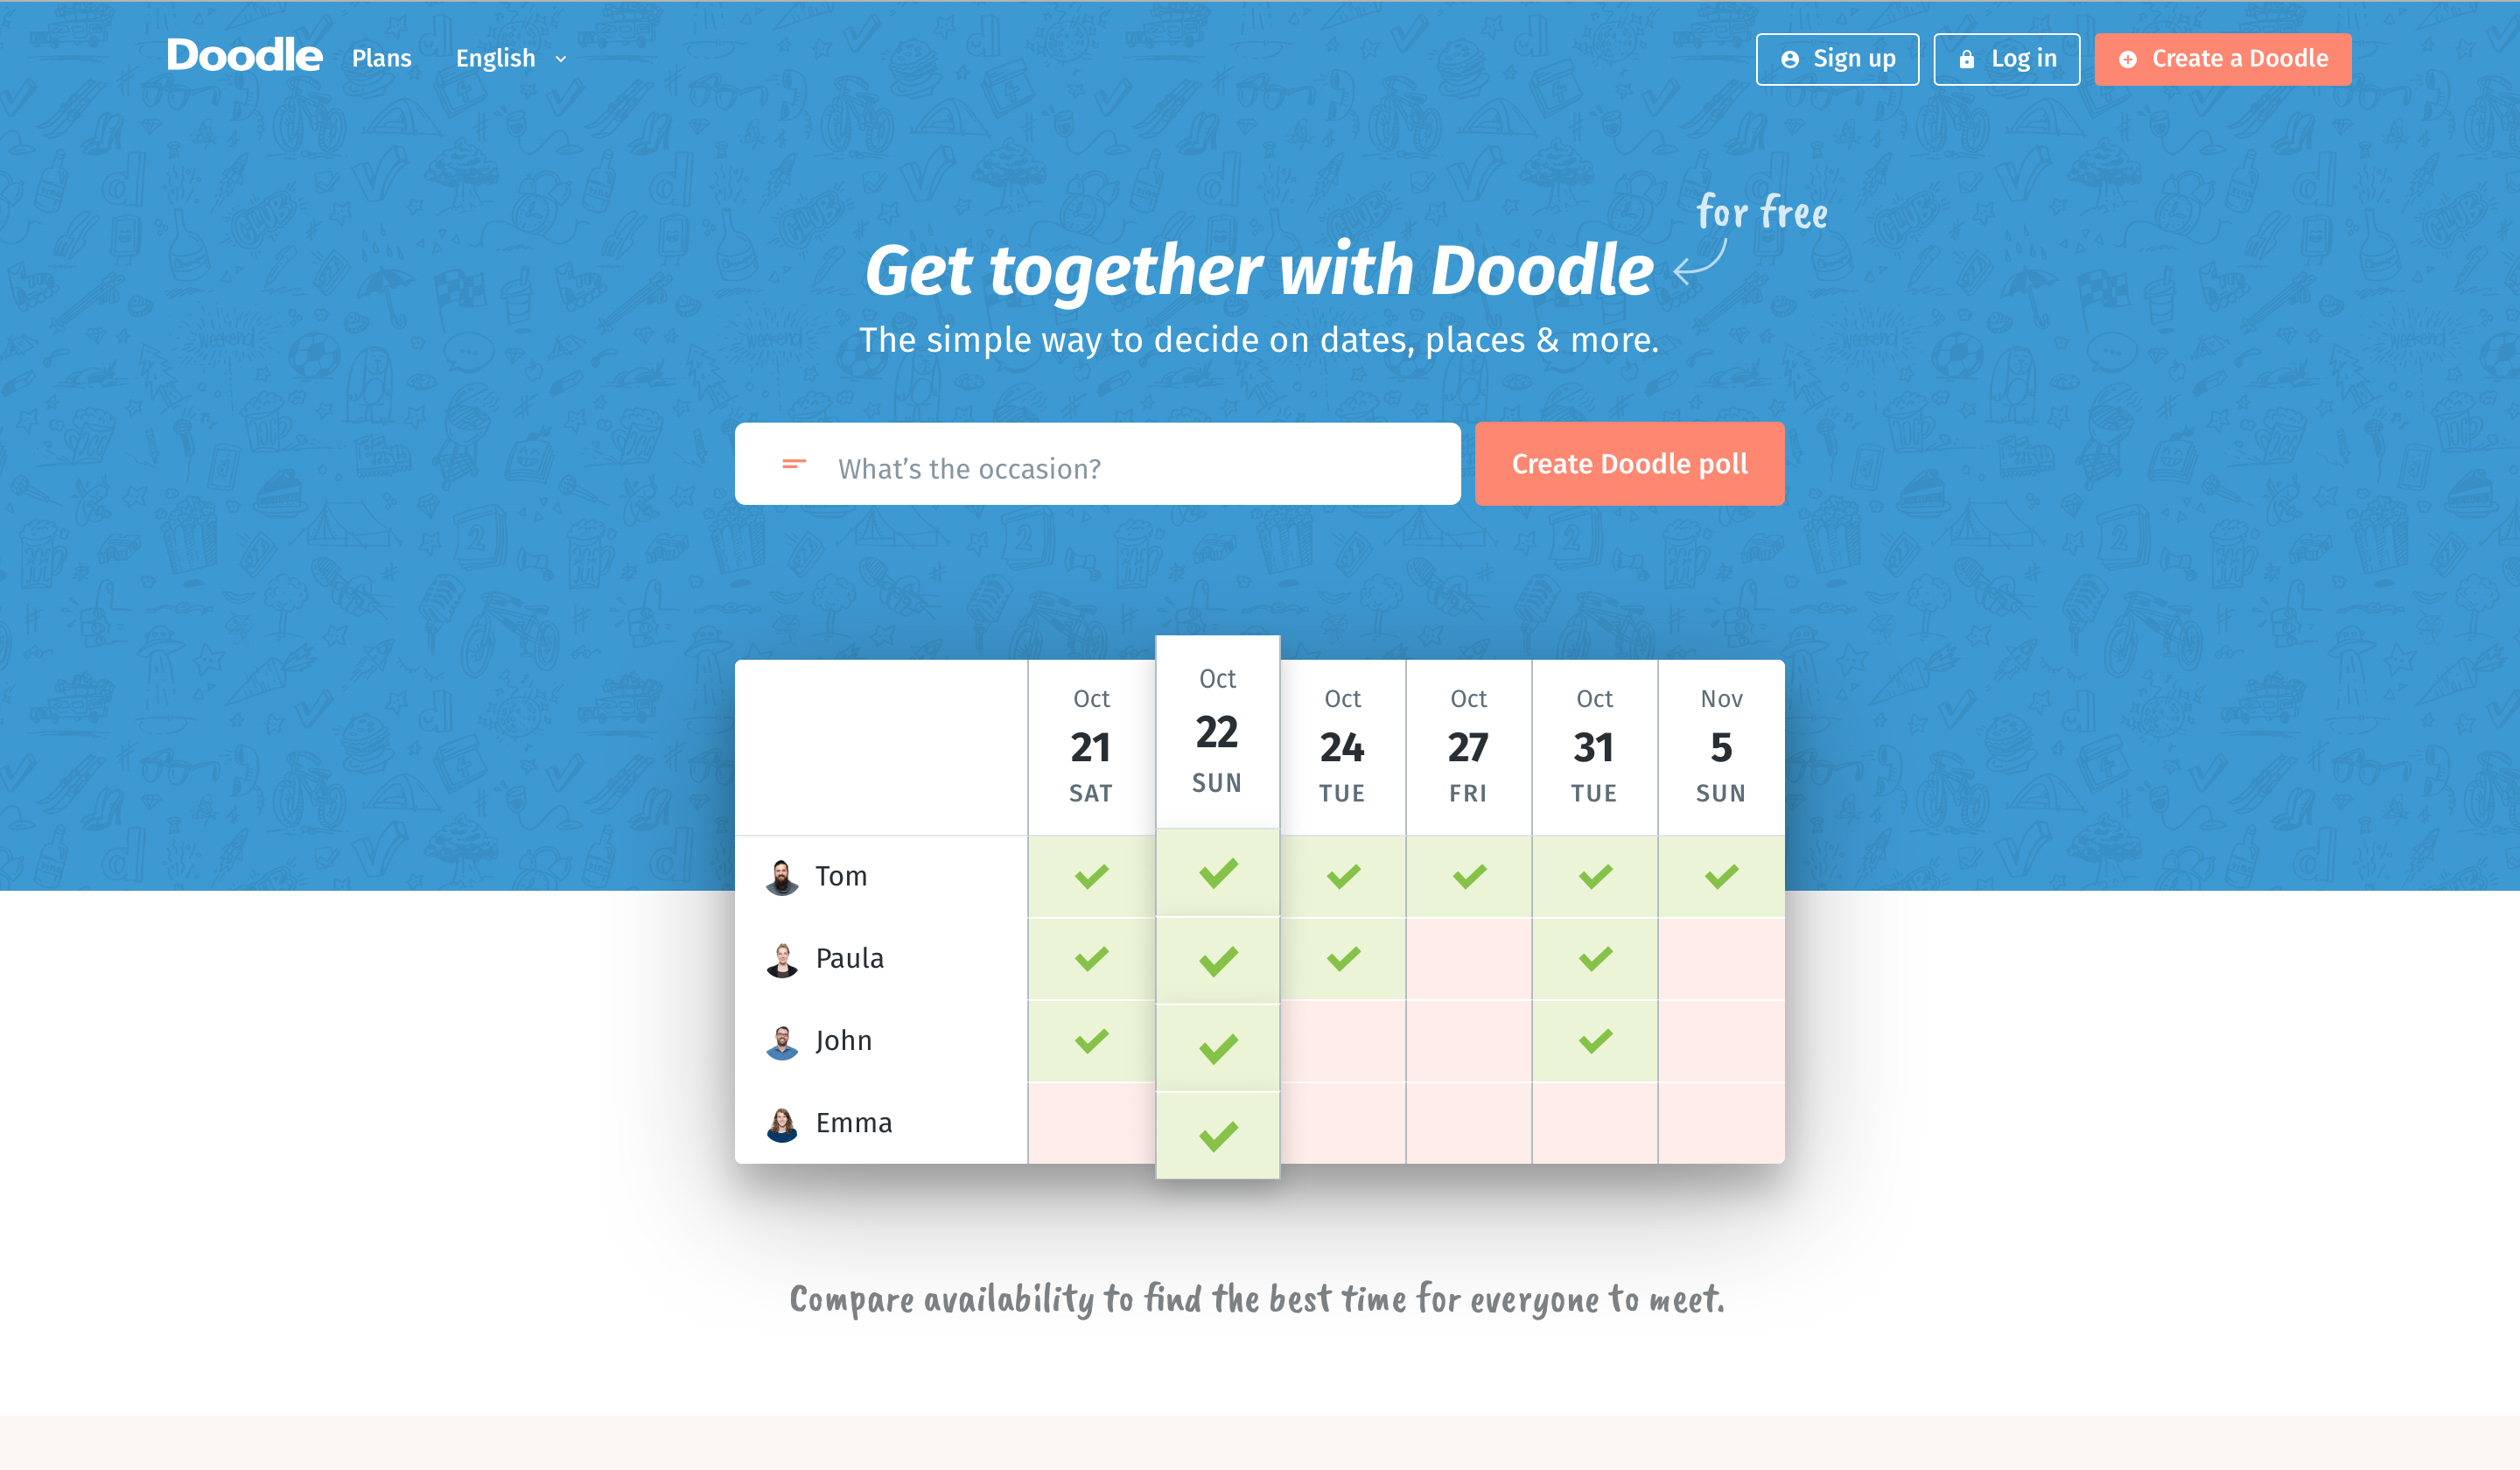
\includegraphics[width=\columnwidth]{{doodle/index.png}}
\label{fig:DOOD_index}
\caption{Doodle homepage}
\end{figure}

\begin{figure}[H]
\centering
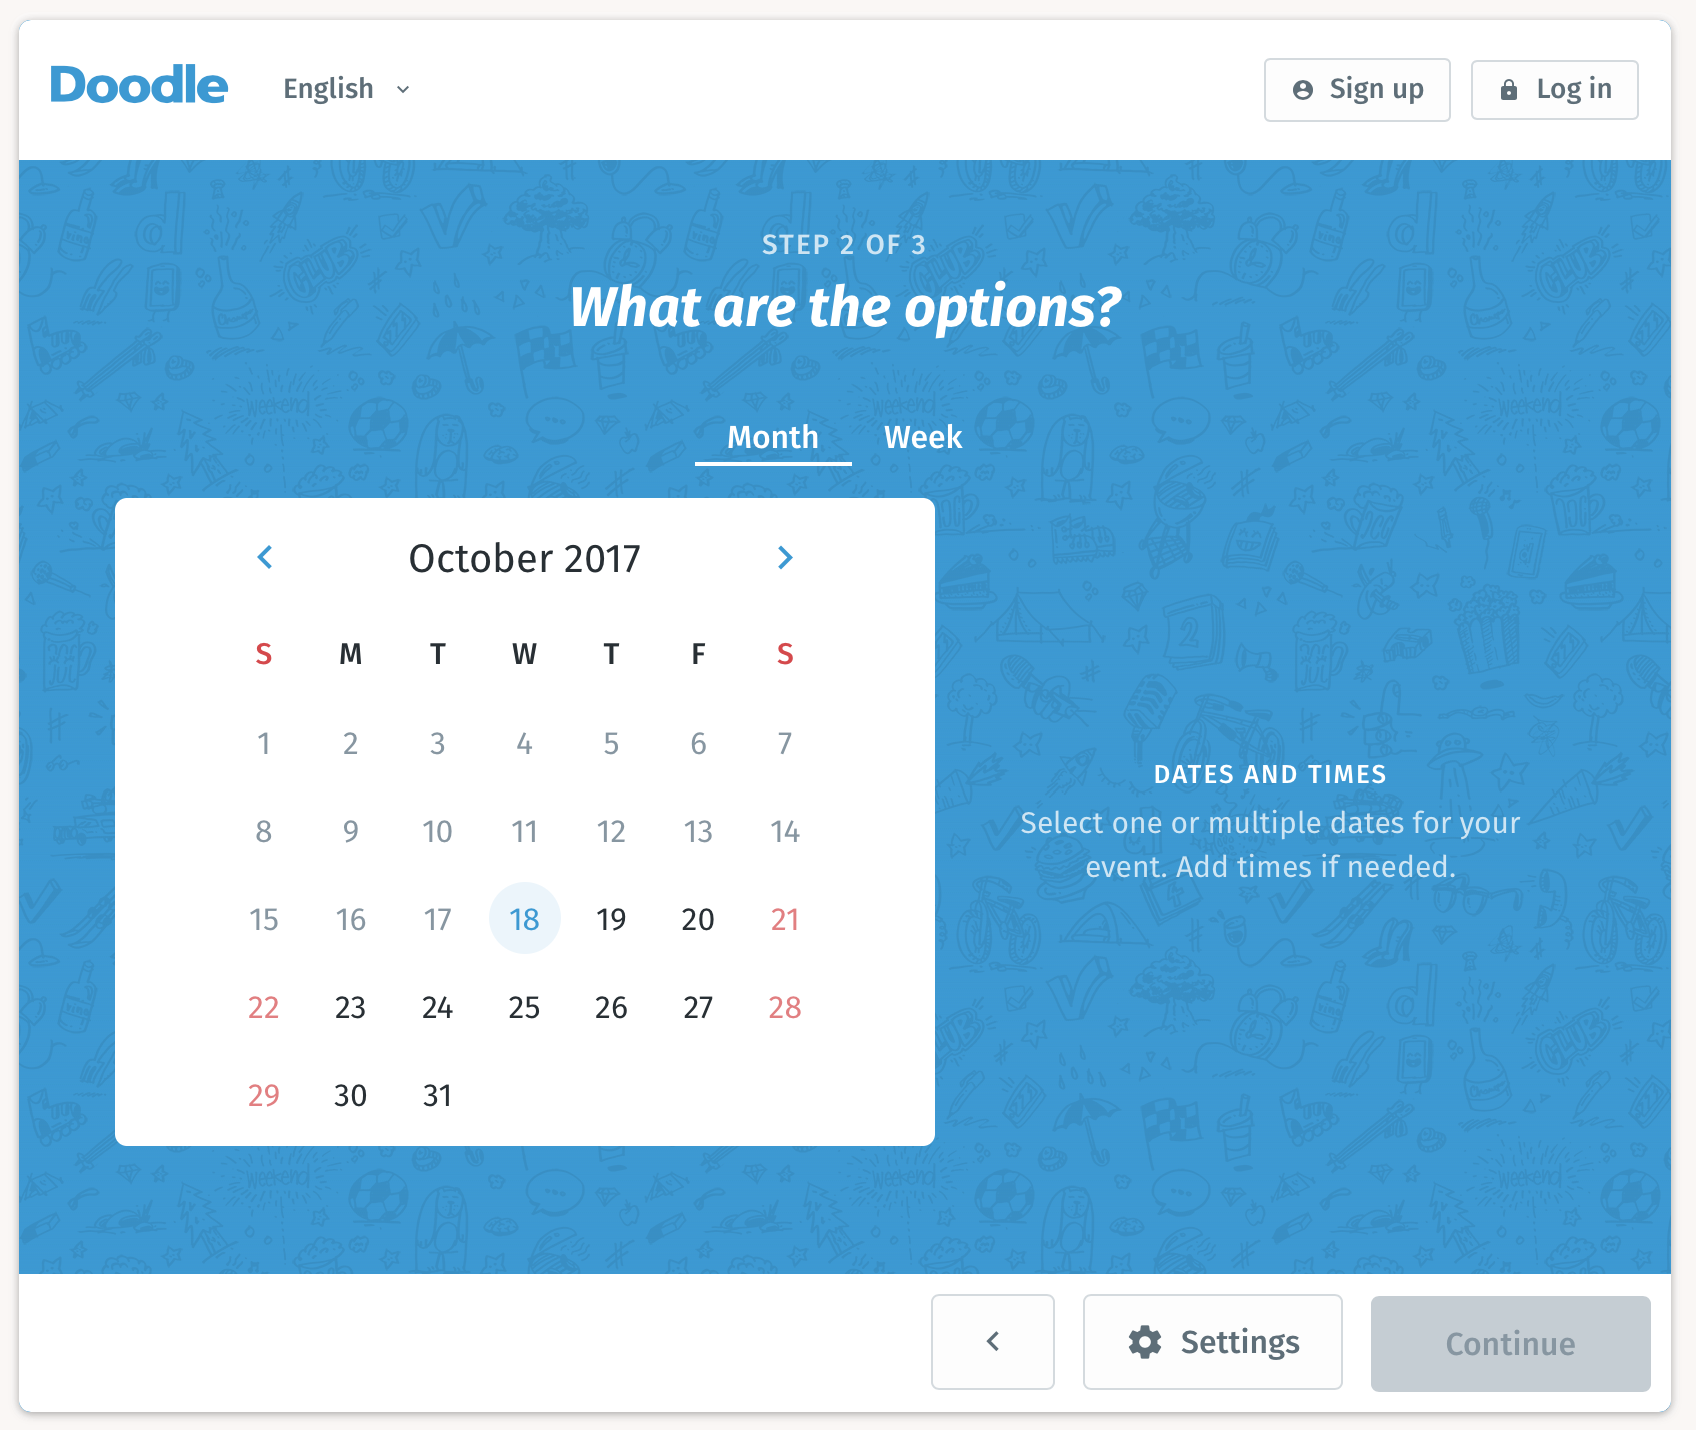
\includegraphics[width=\columnwidth]{{doodle/create-2.png}}
\caption{Create event dialog}
\end{figure}

\begin{figure}[H]
\centering
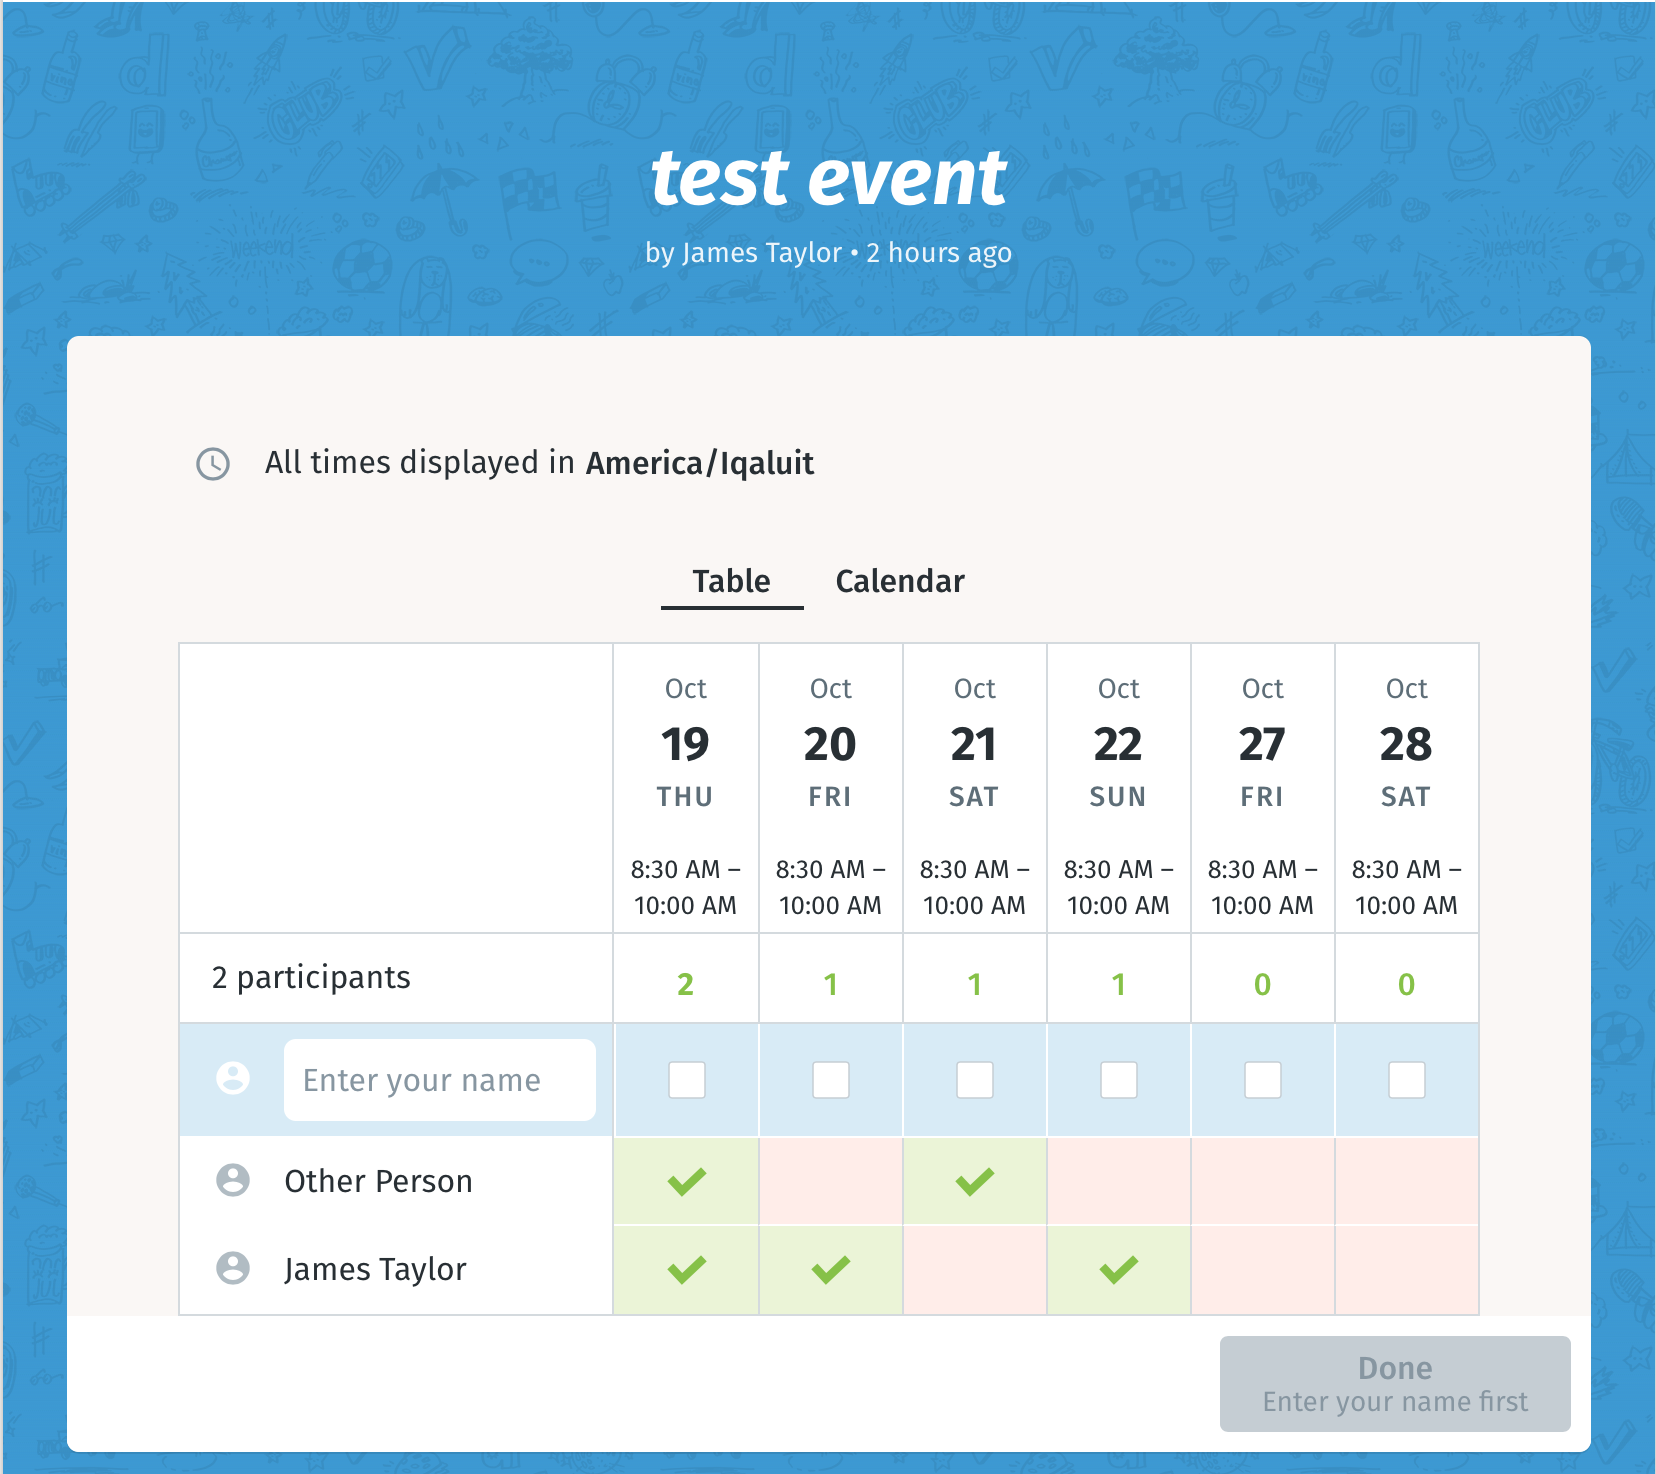
\includegraphics[width=\columnwidth]{{doodle/event.png}}
\caption{Event homepage}
\end{figure}

\begin{figure}[H]
\centering
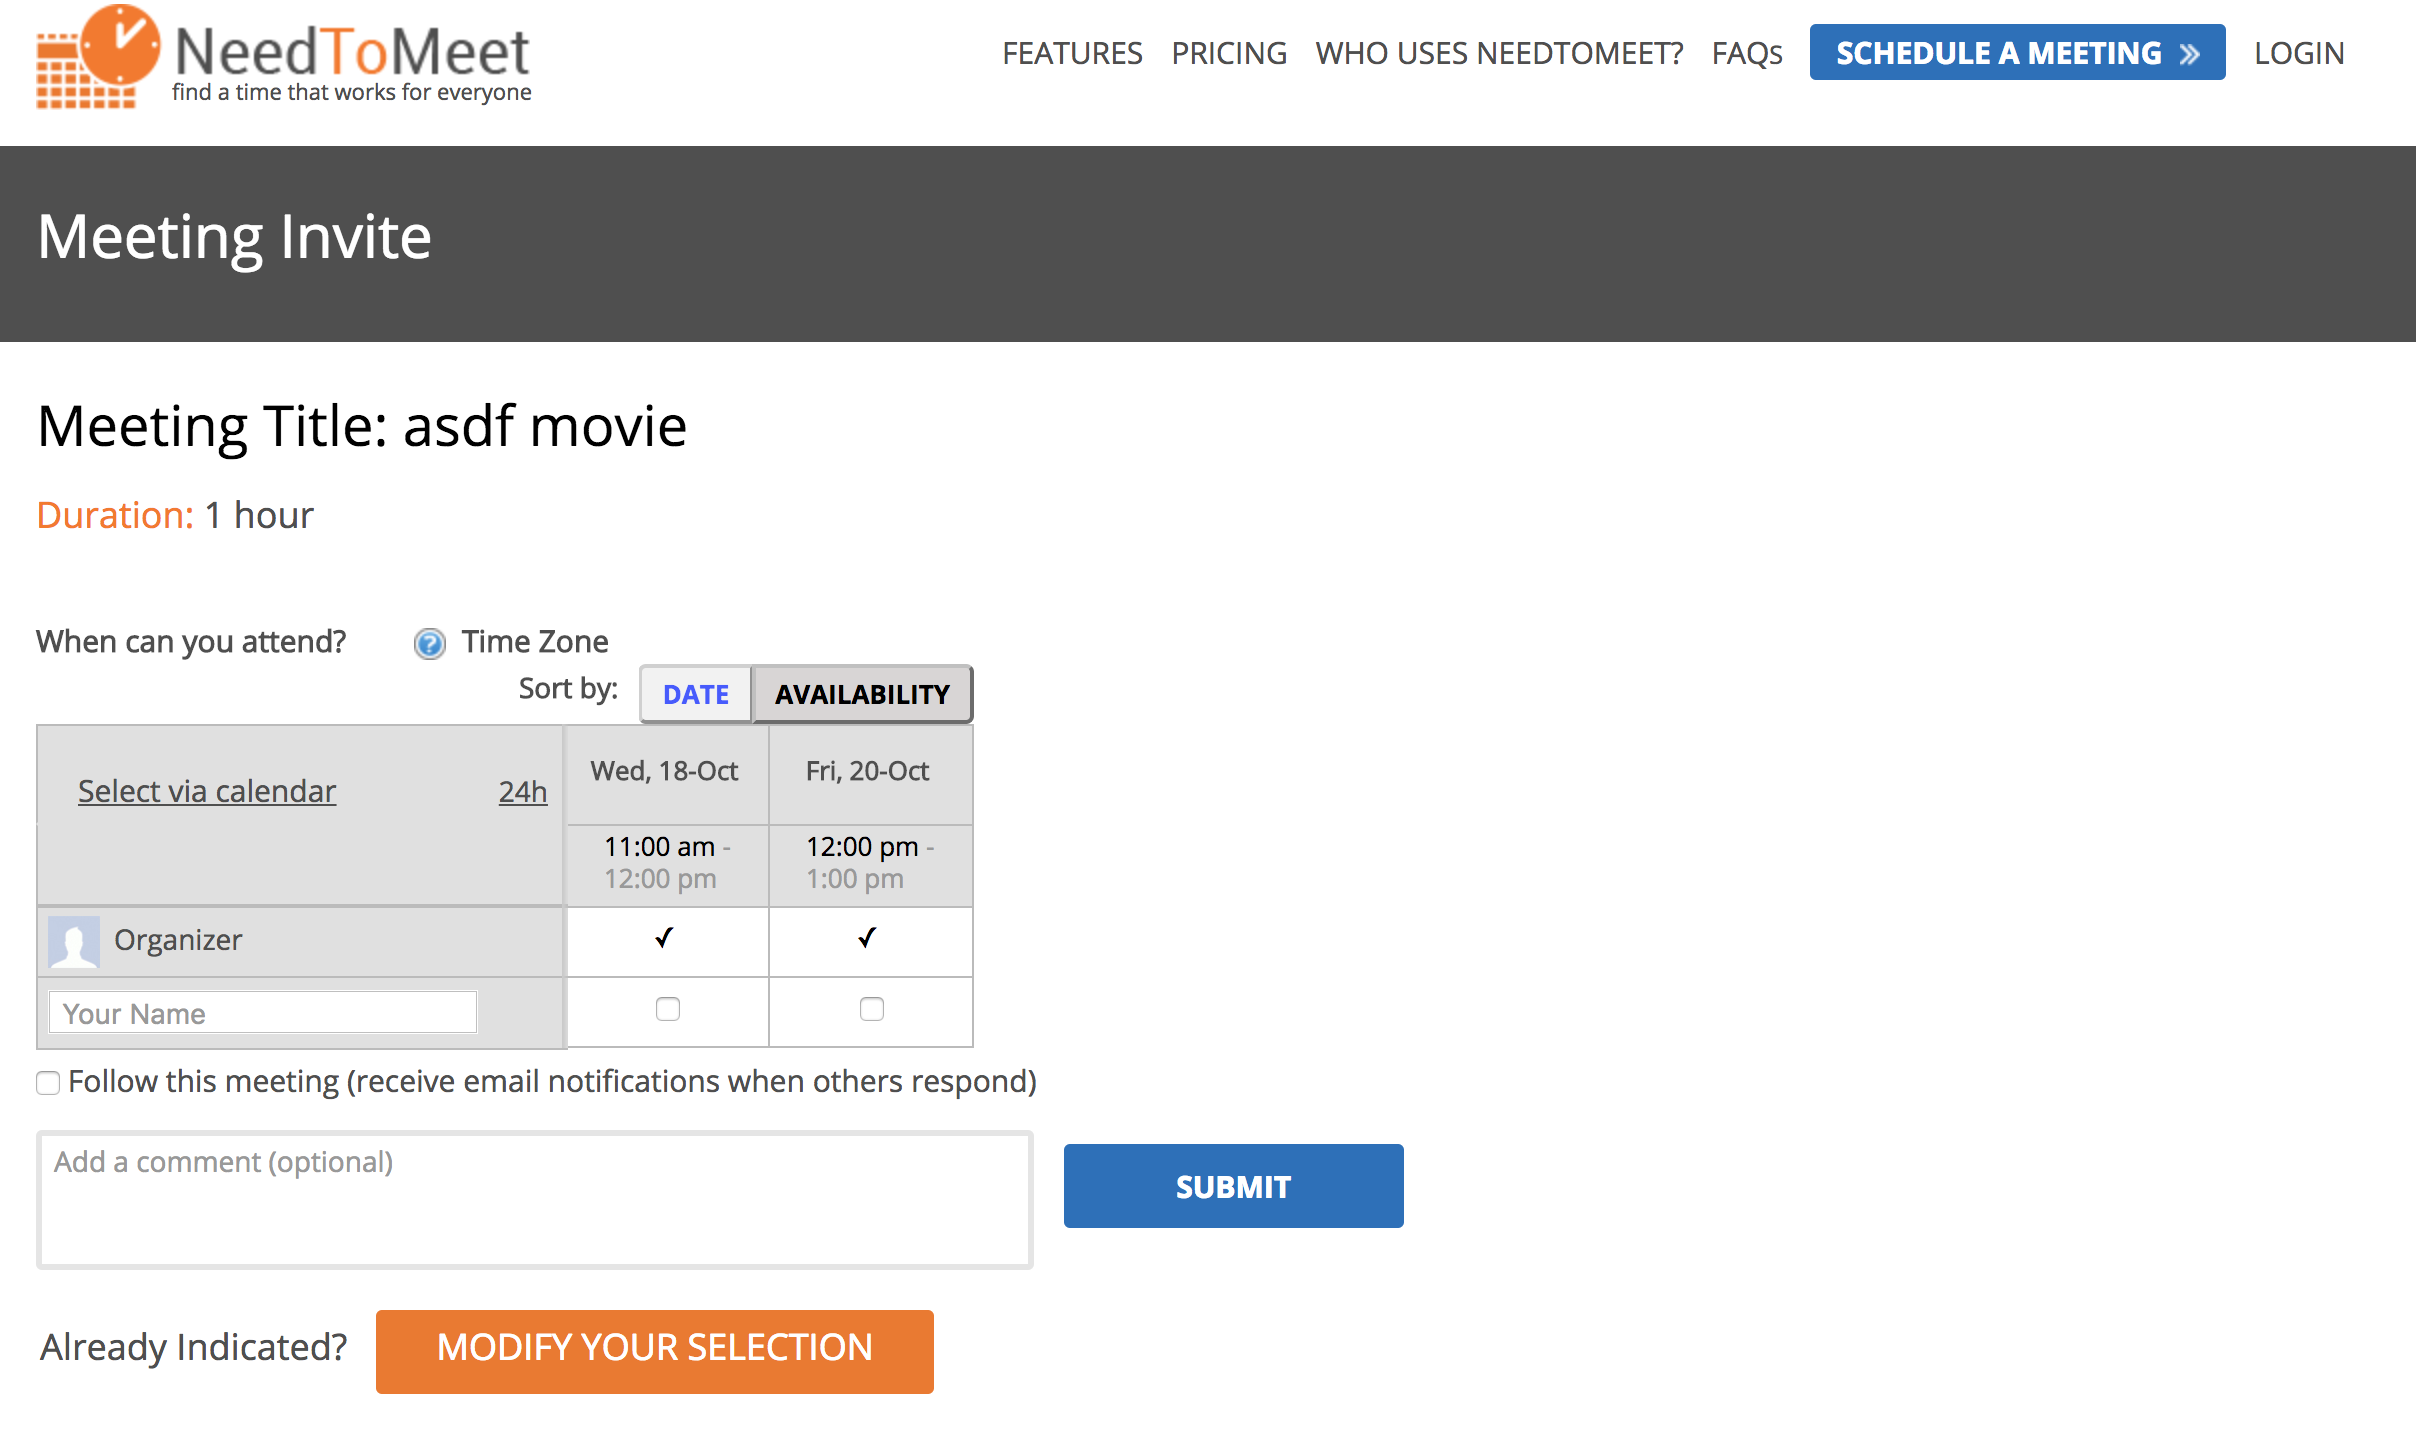
\includegraphics[width=\columnwidth]{{figures/NeedToMeet/Creator_Images/1.png}}
\caption{Need To Meet Homepage}
\end{figure}
%%%%%%

\begin{figure}[H]
\centering
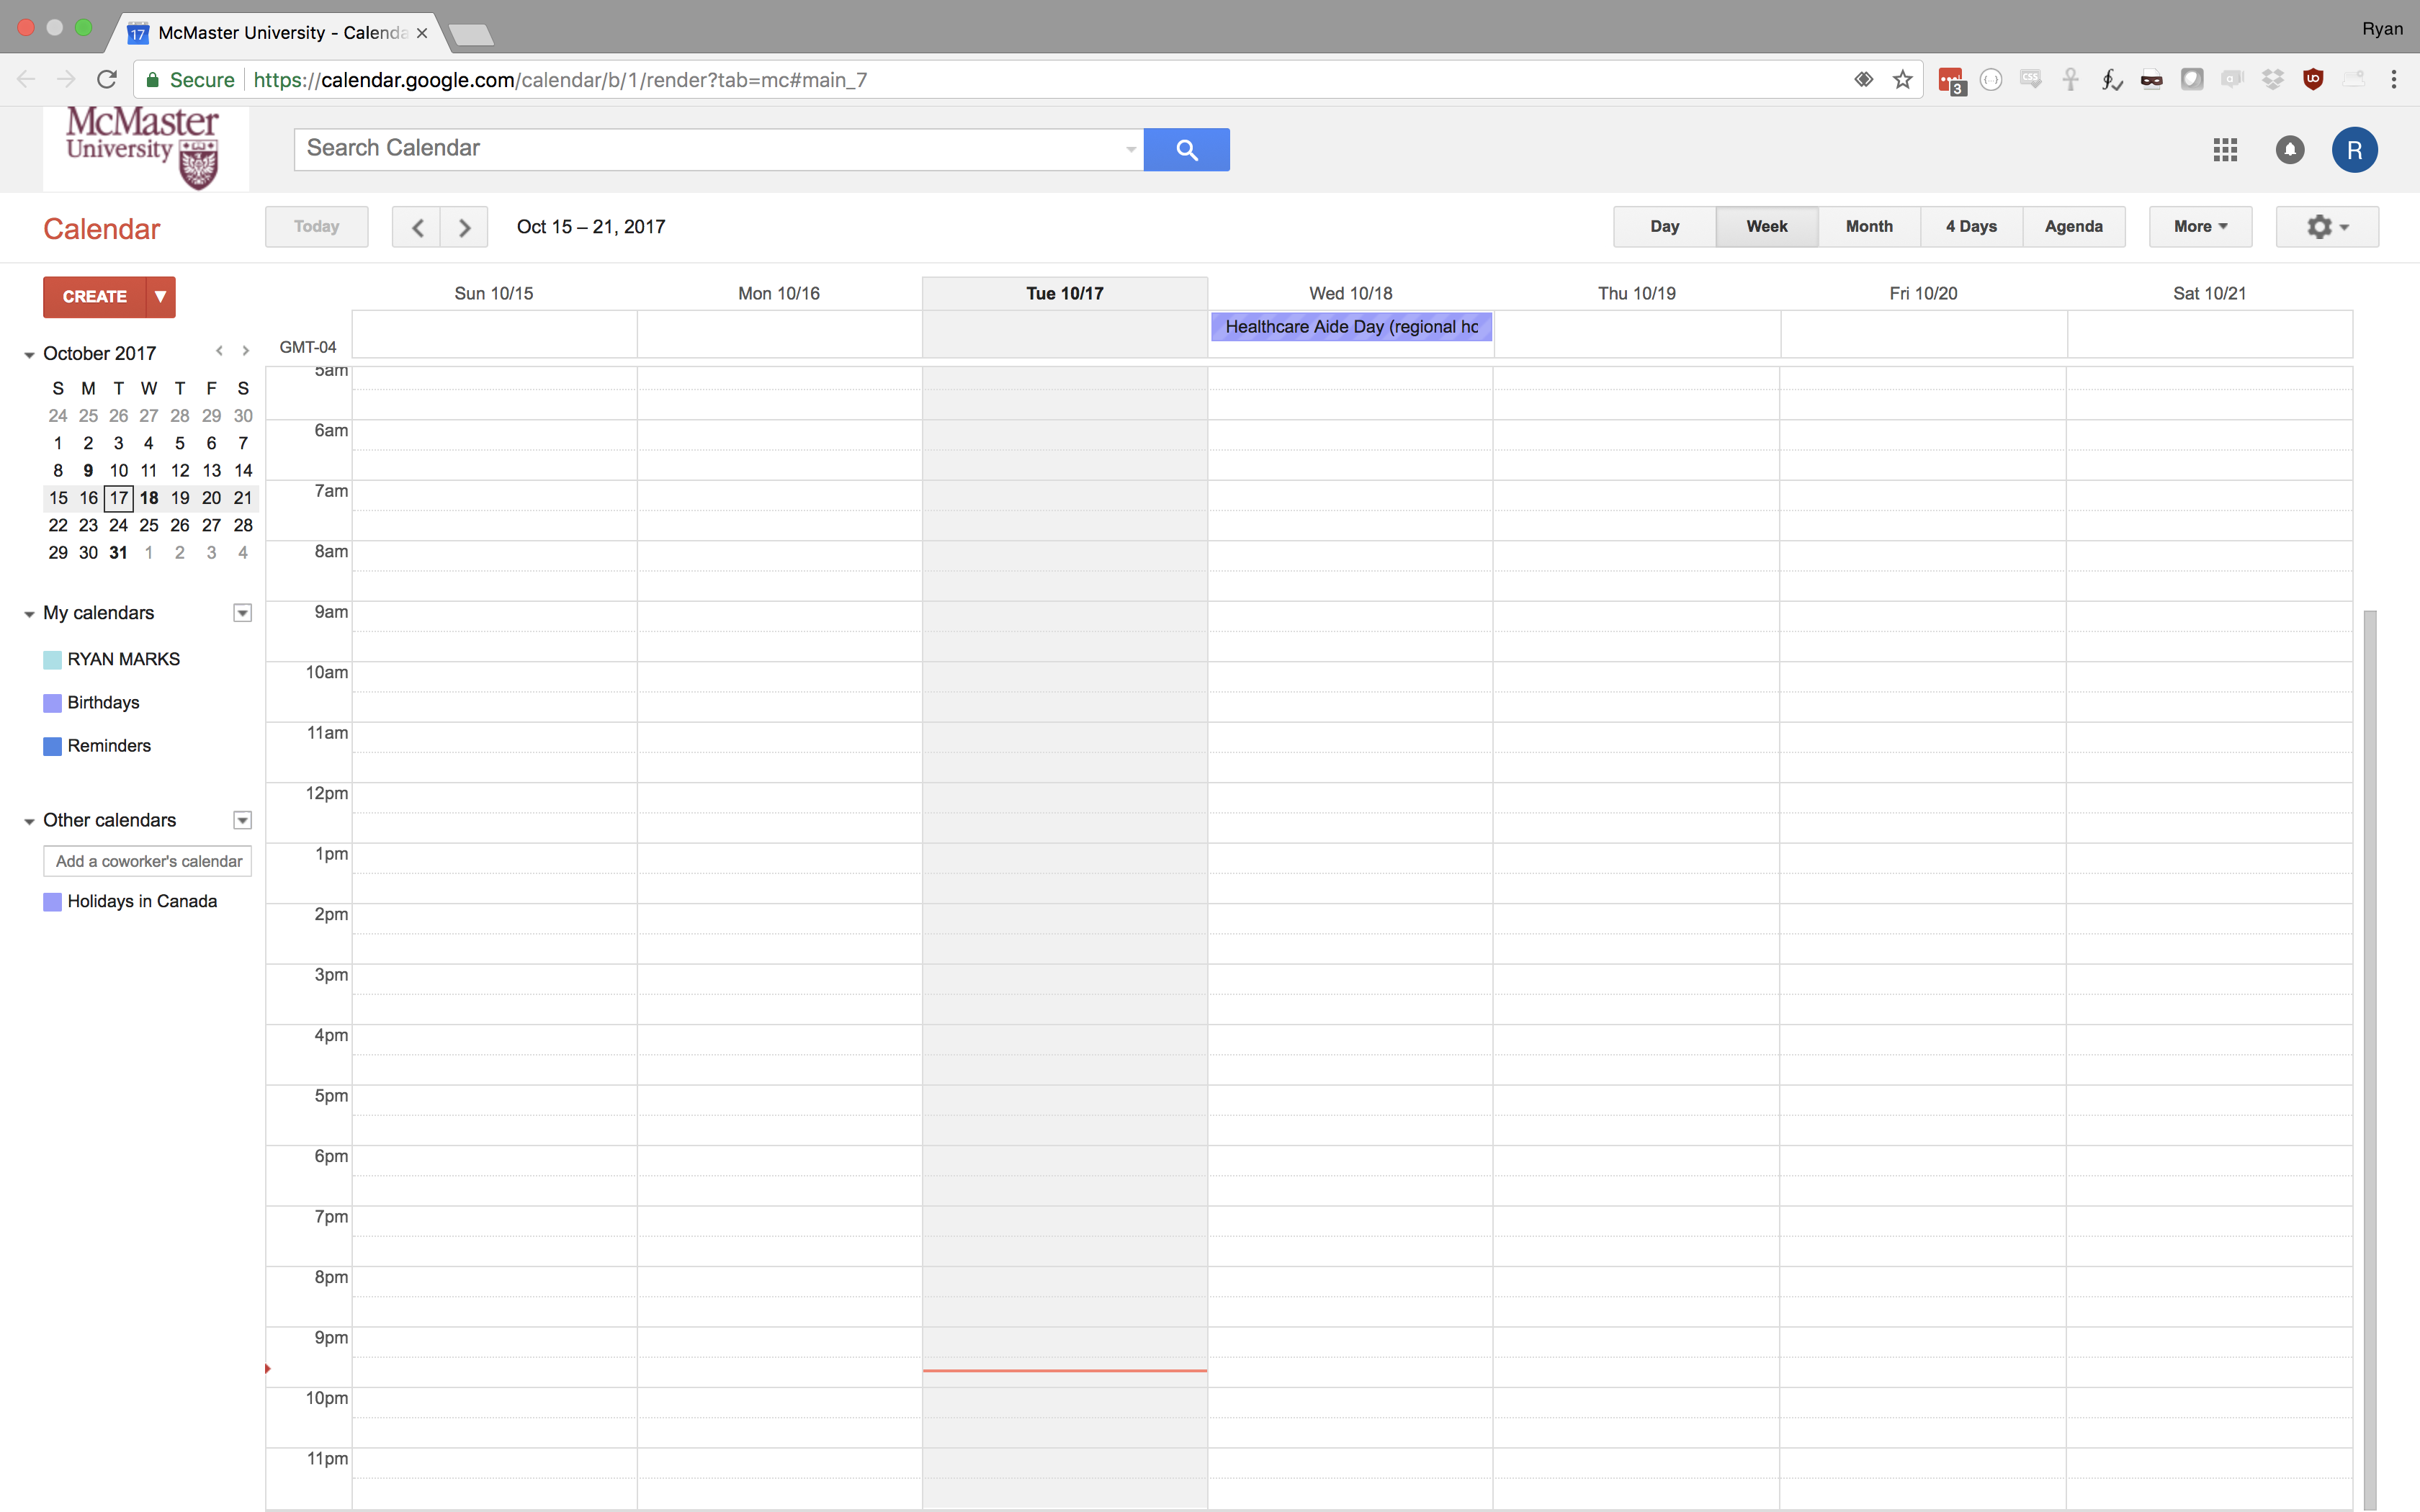
\includegraphics[width=\columnwidth]{{google/Invite1_1}}
\caption{Subtask 1.1 of the invitation procedure for Google Calendar}
\end{figure}

\begin{figure}[H]
\centering
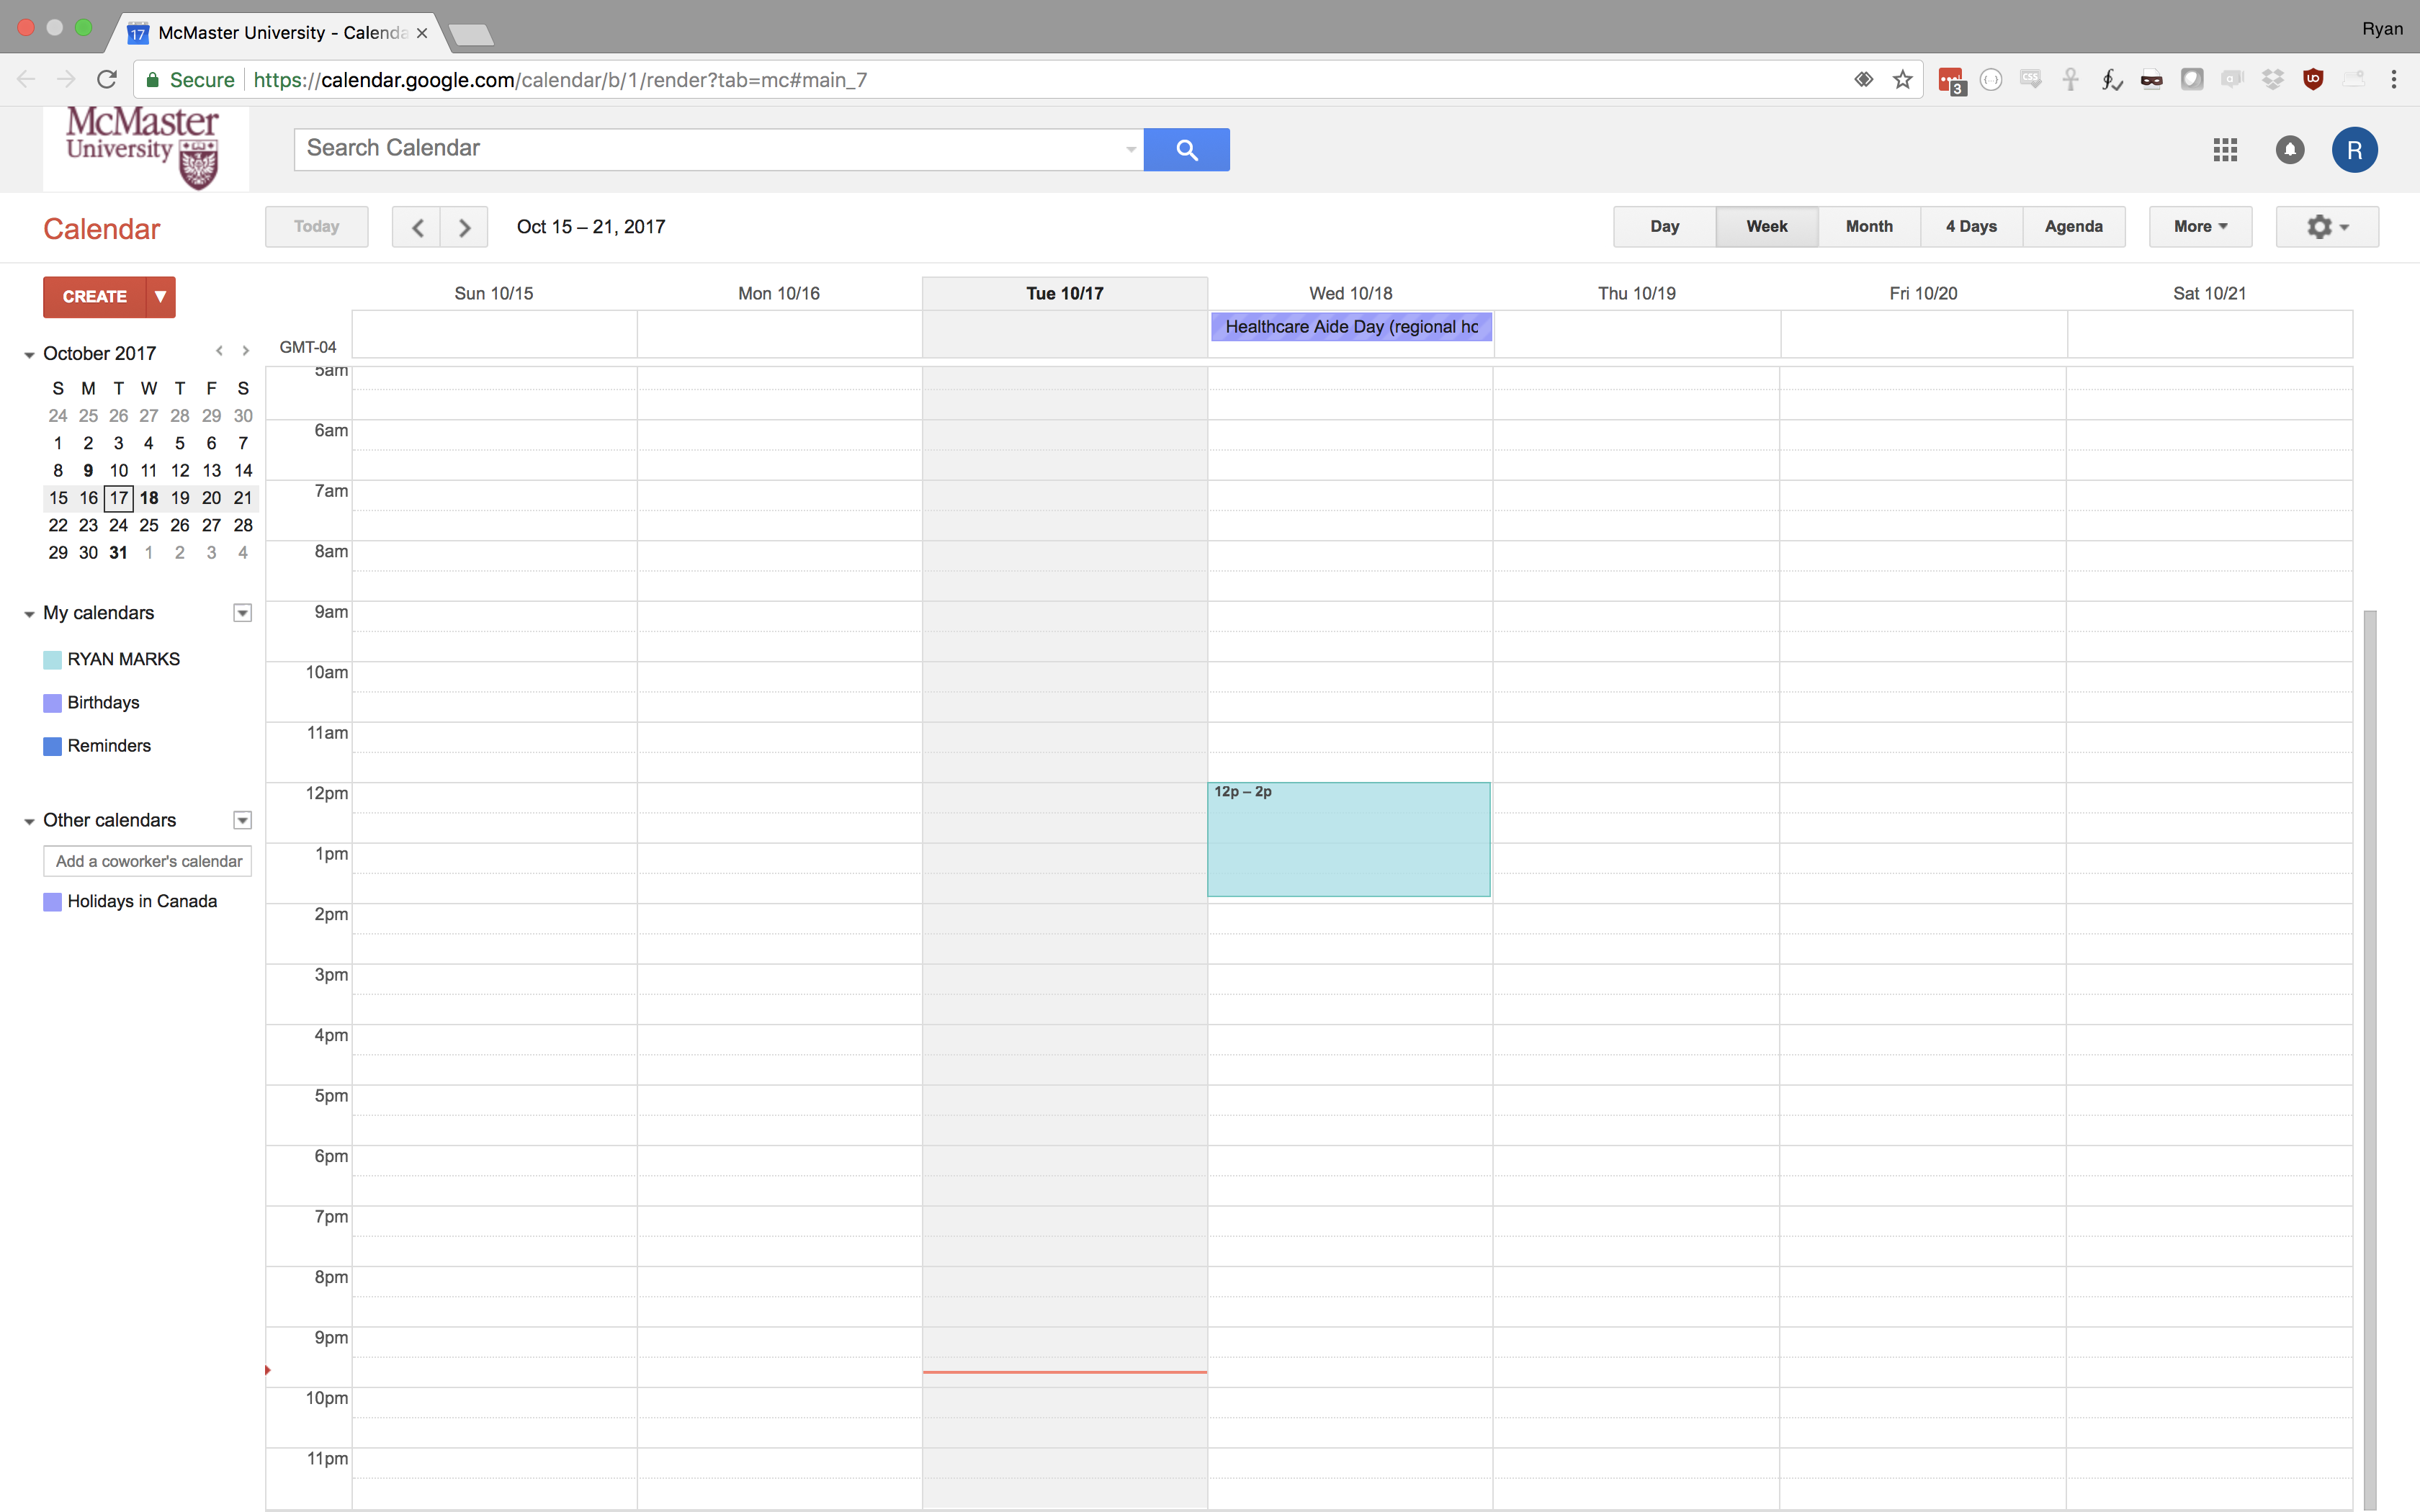
\includegraphics[width=\columnwidth]{{google/Invite1_2.png}}
\caption{Subtask 1.2 of the invitation procedure for Google Calendar}
\end{figure}

\begin{figure}[H]
\centering
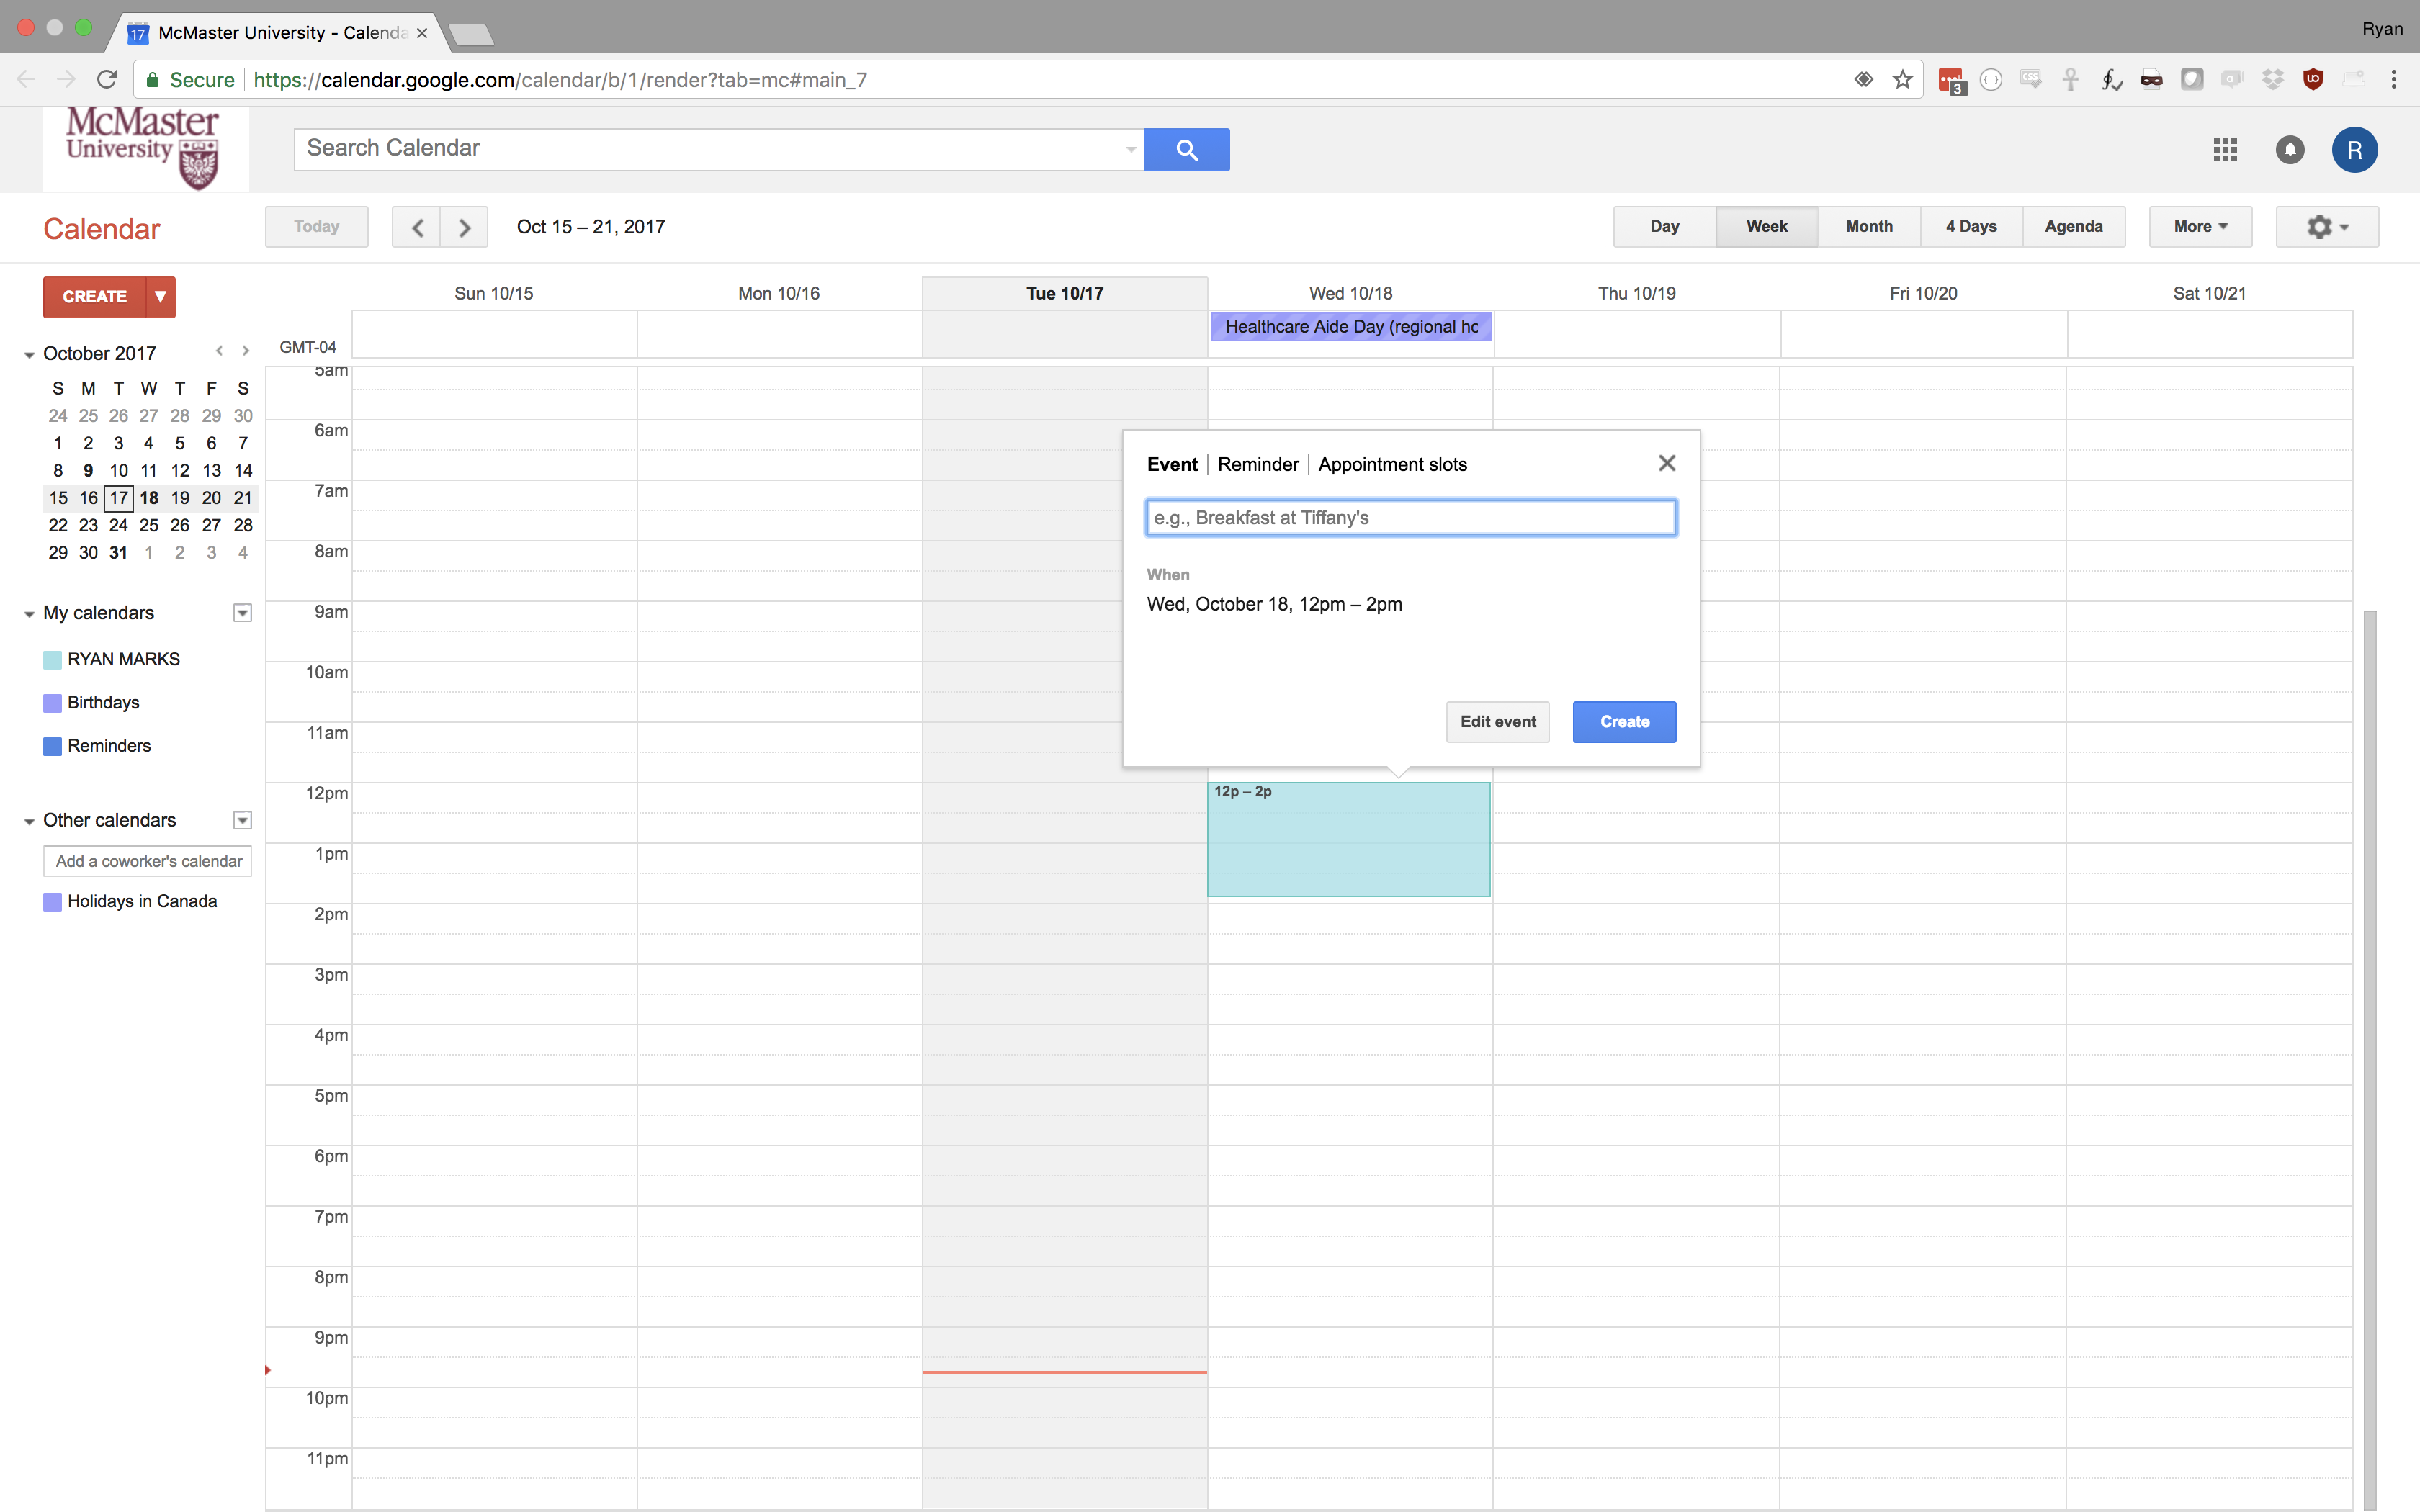
\includegraphics[width=\columnwidth]{{google/Invite1_3.png}}
\caption{Befort subtask 1.3 of the invitation procedure for Google Calendar}
\end{figure}

\begin{figure}[H]
\centering
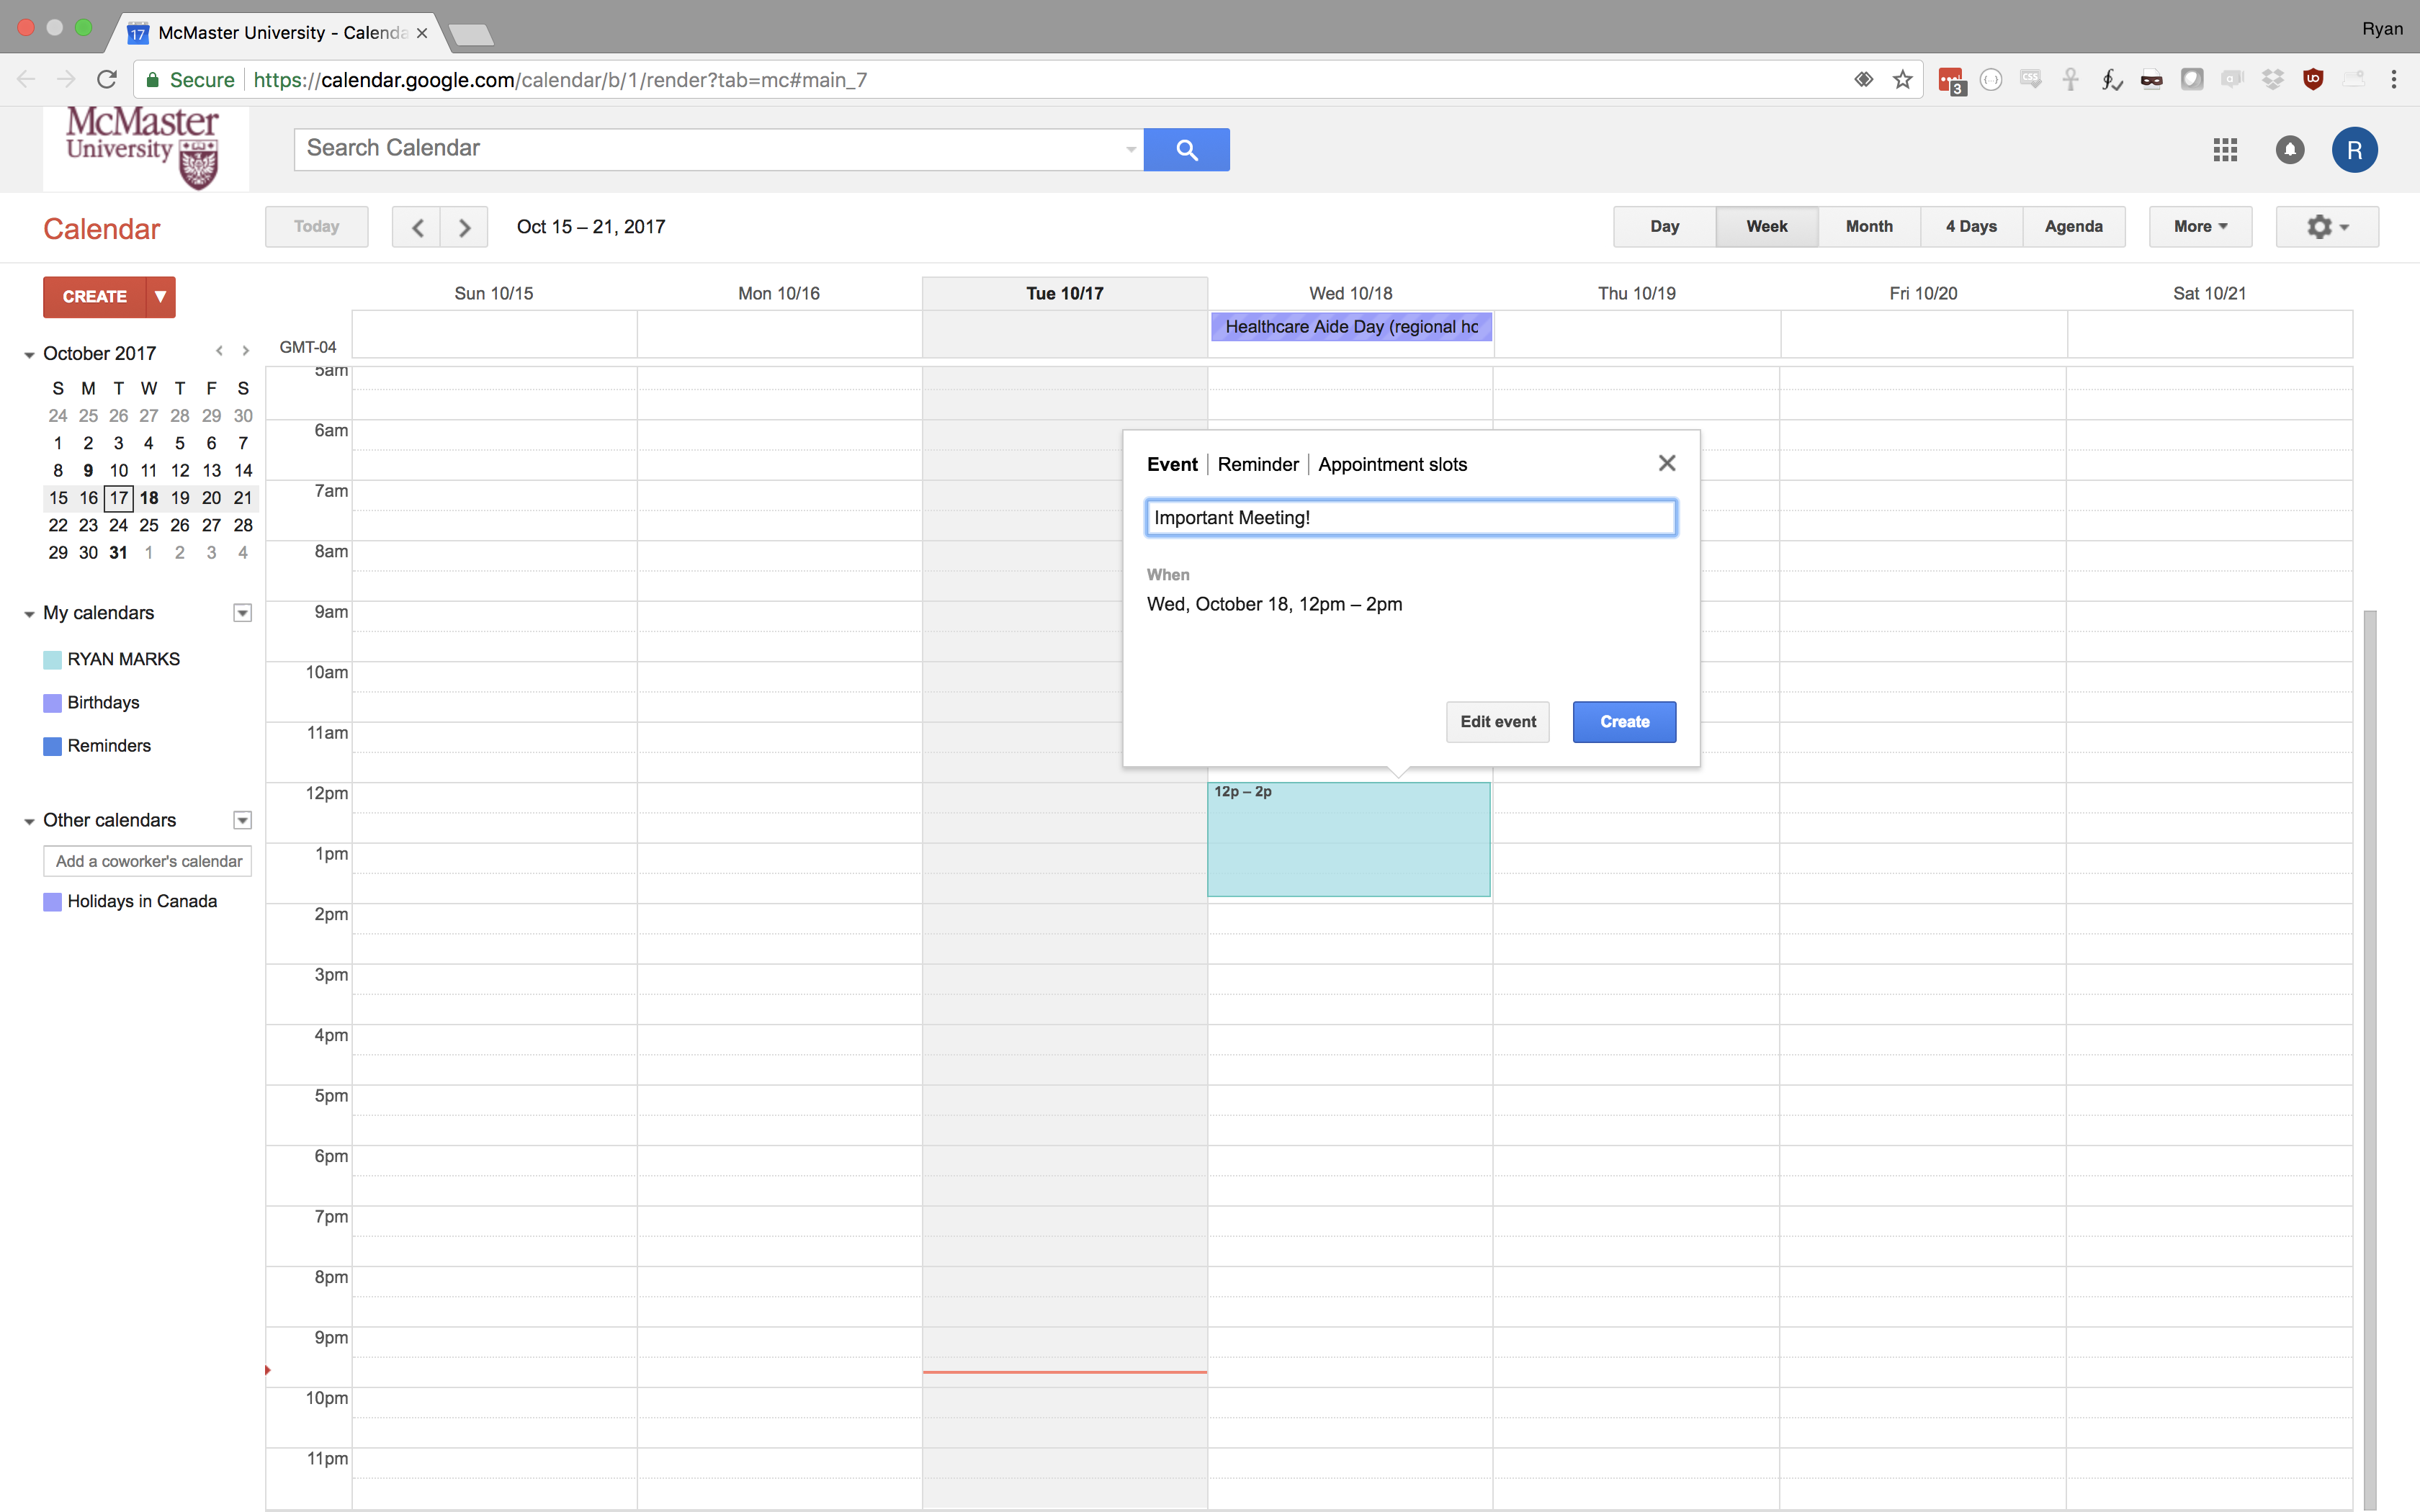
\includegraphics[width=\columnwidth]{{google/Invite1_3end.png}}
\caption{After subtask 1.3 of the invitation procedure for Google Calendar}
\end{figure}

\begin{figure}[H]
\centering
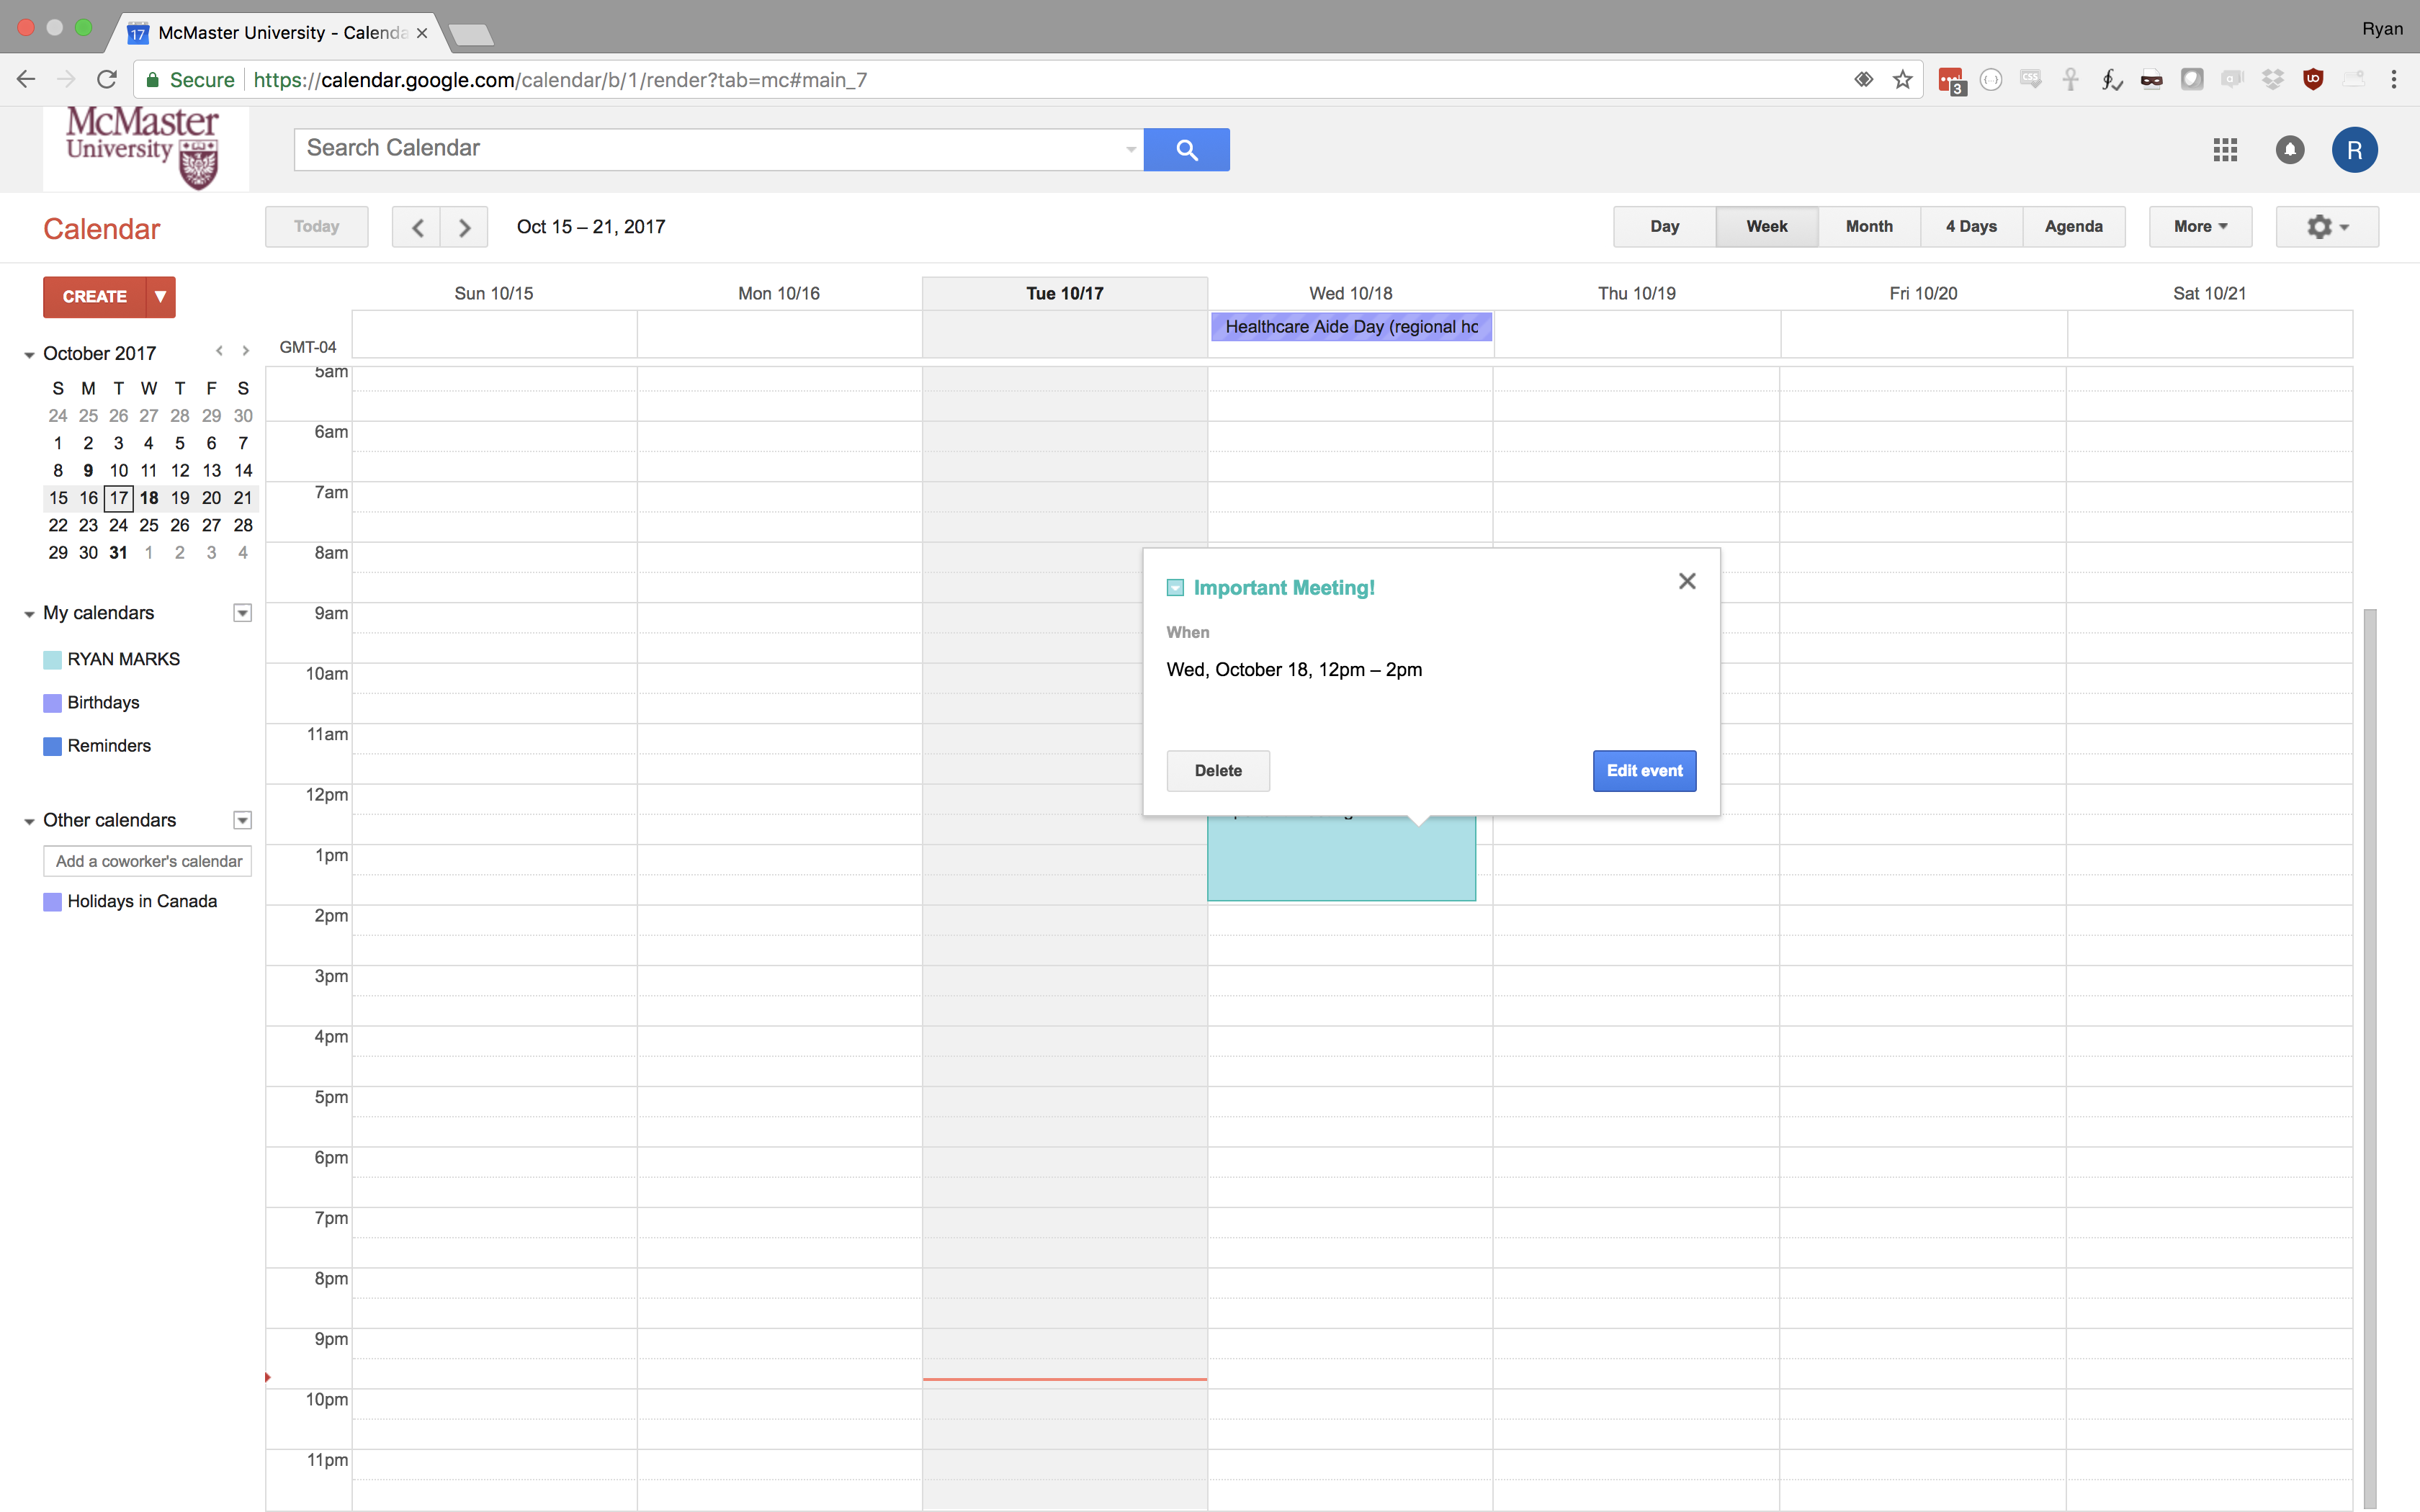
\includegraphics[width=\columnwidth]{{google/Invite2_1.png}}
\caption{Before subtask 2.1 of the invitation procedure for Google Calendar}
\end{figure}

\begin{figure}[H]
\centering
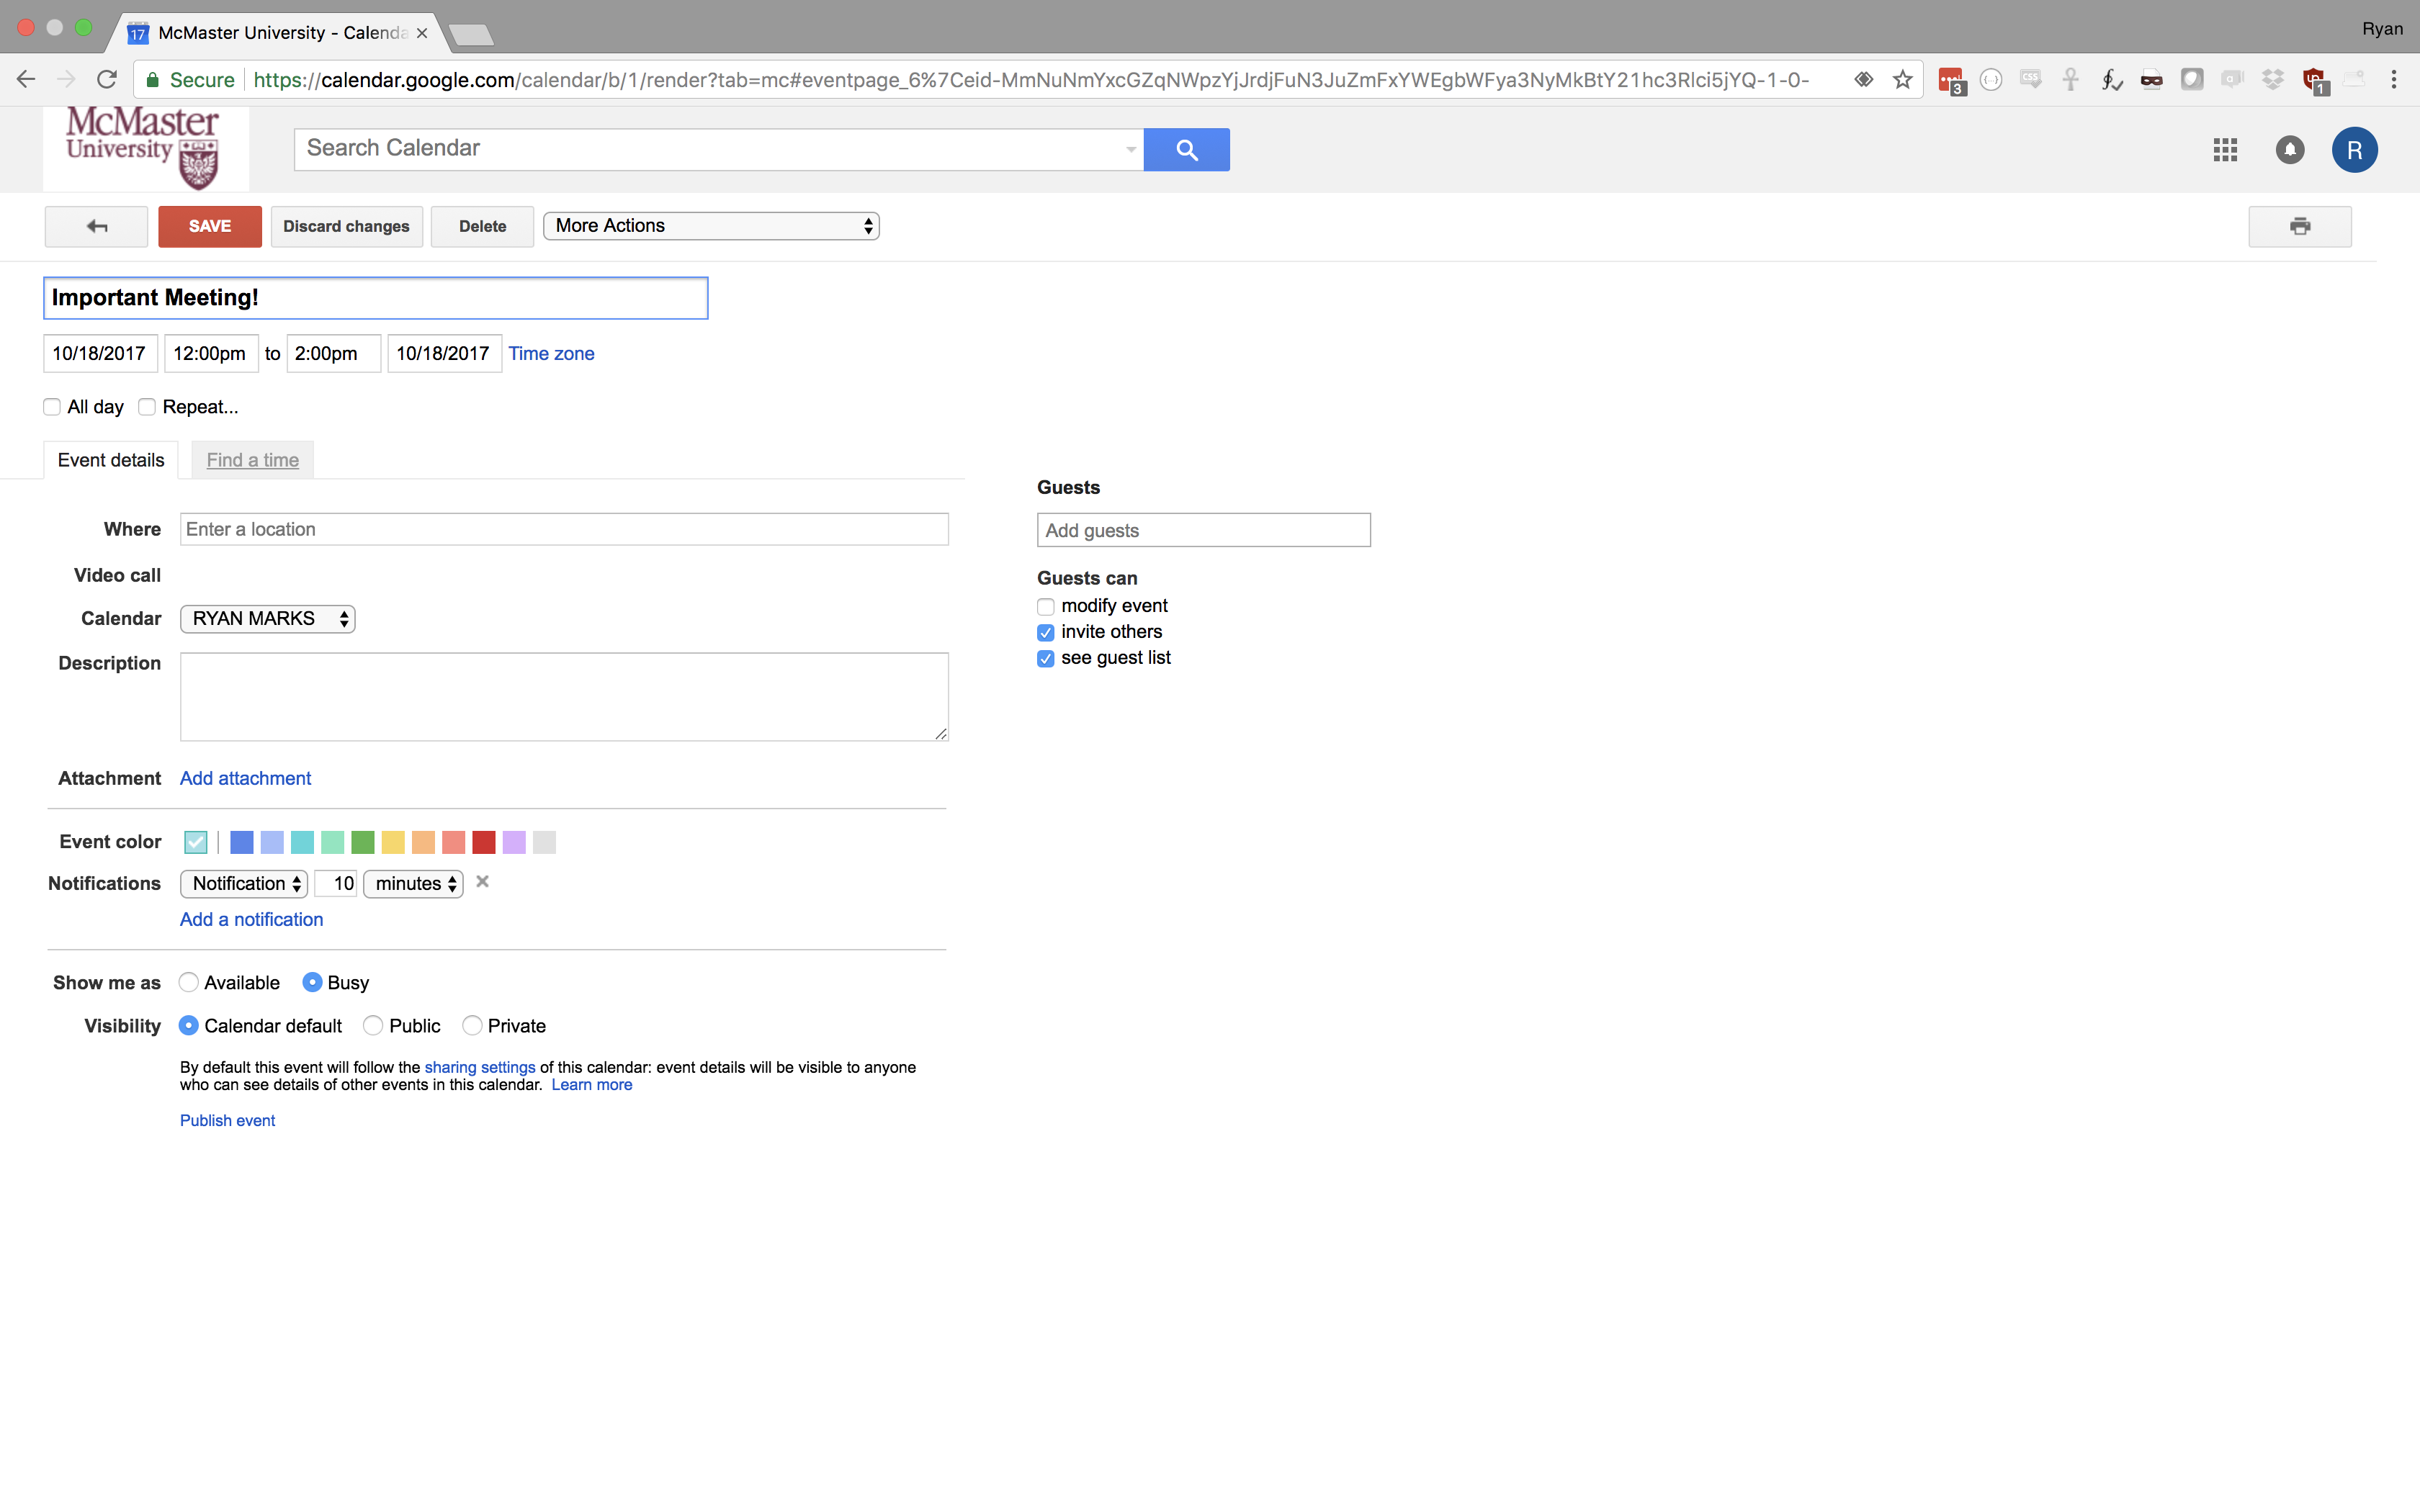
\includegraphics[width=\columnwidth]{{google/Invite2_1end.png}}
\caption{After subtask 2.1 of the invitation procedure for Google Calendar}
\end{figure}

\begin{figure}[H]
\centering
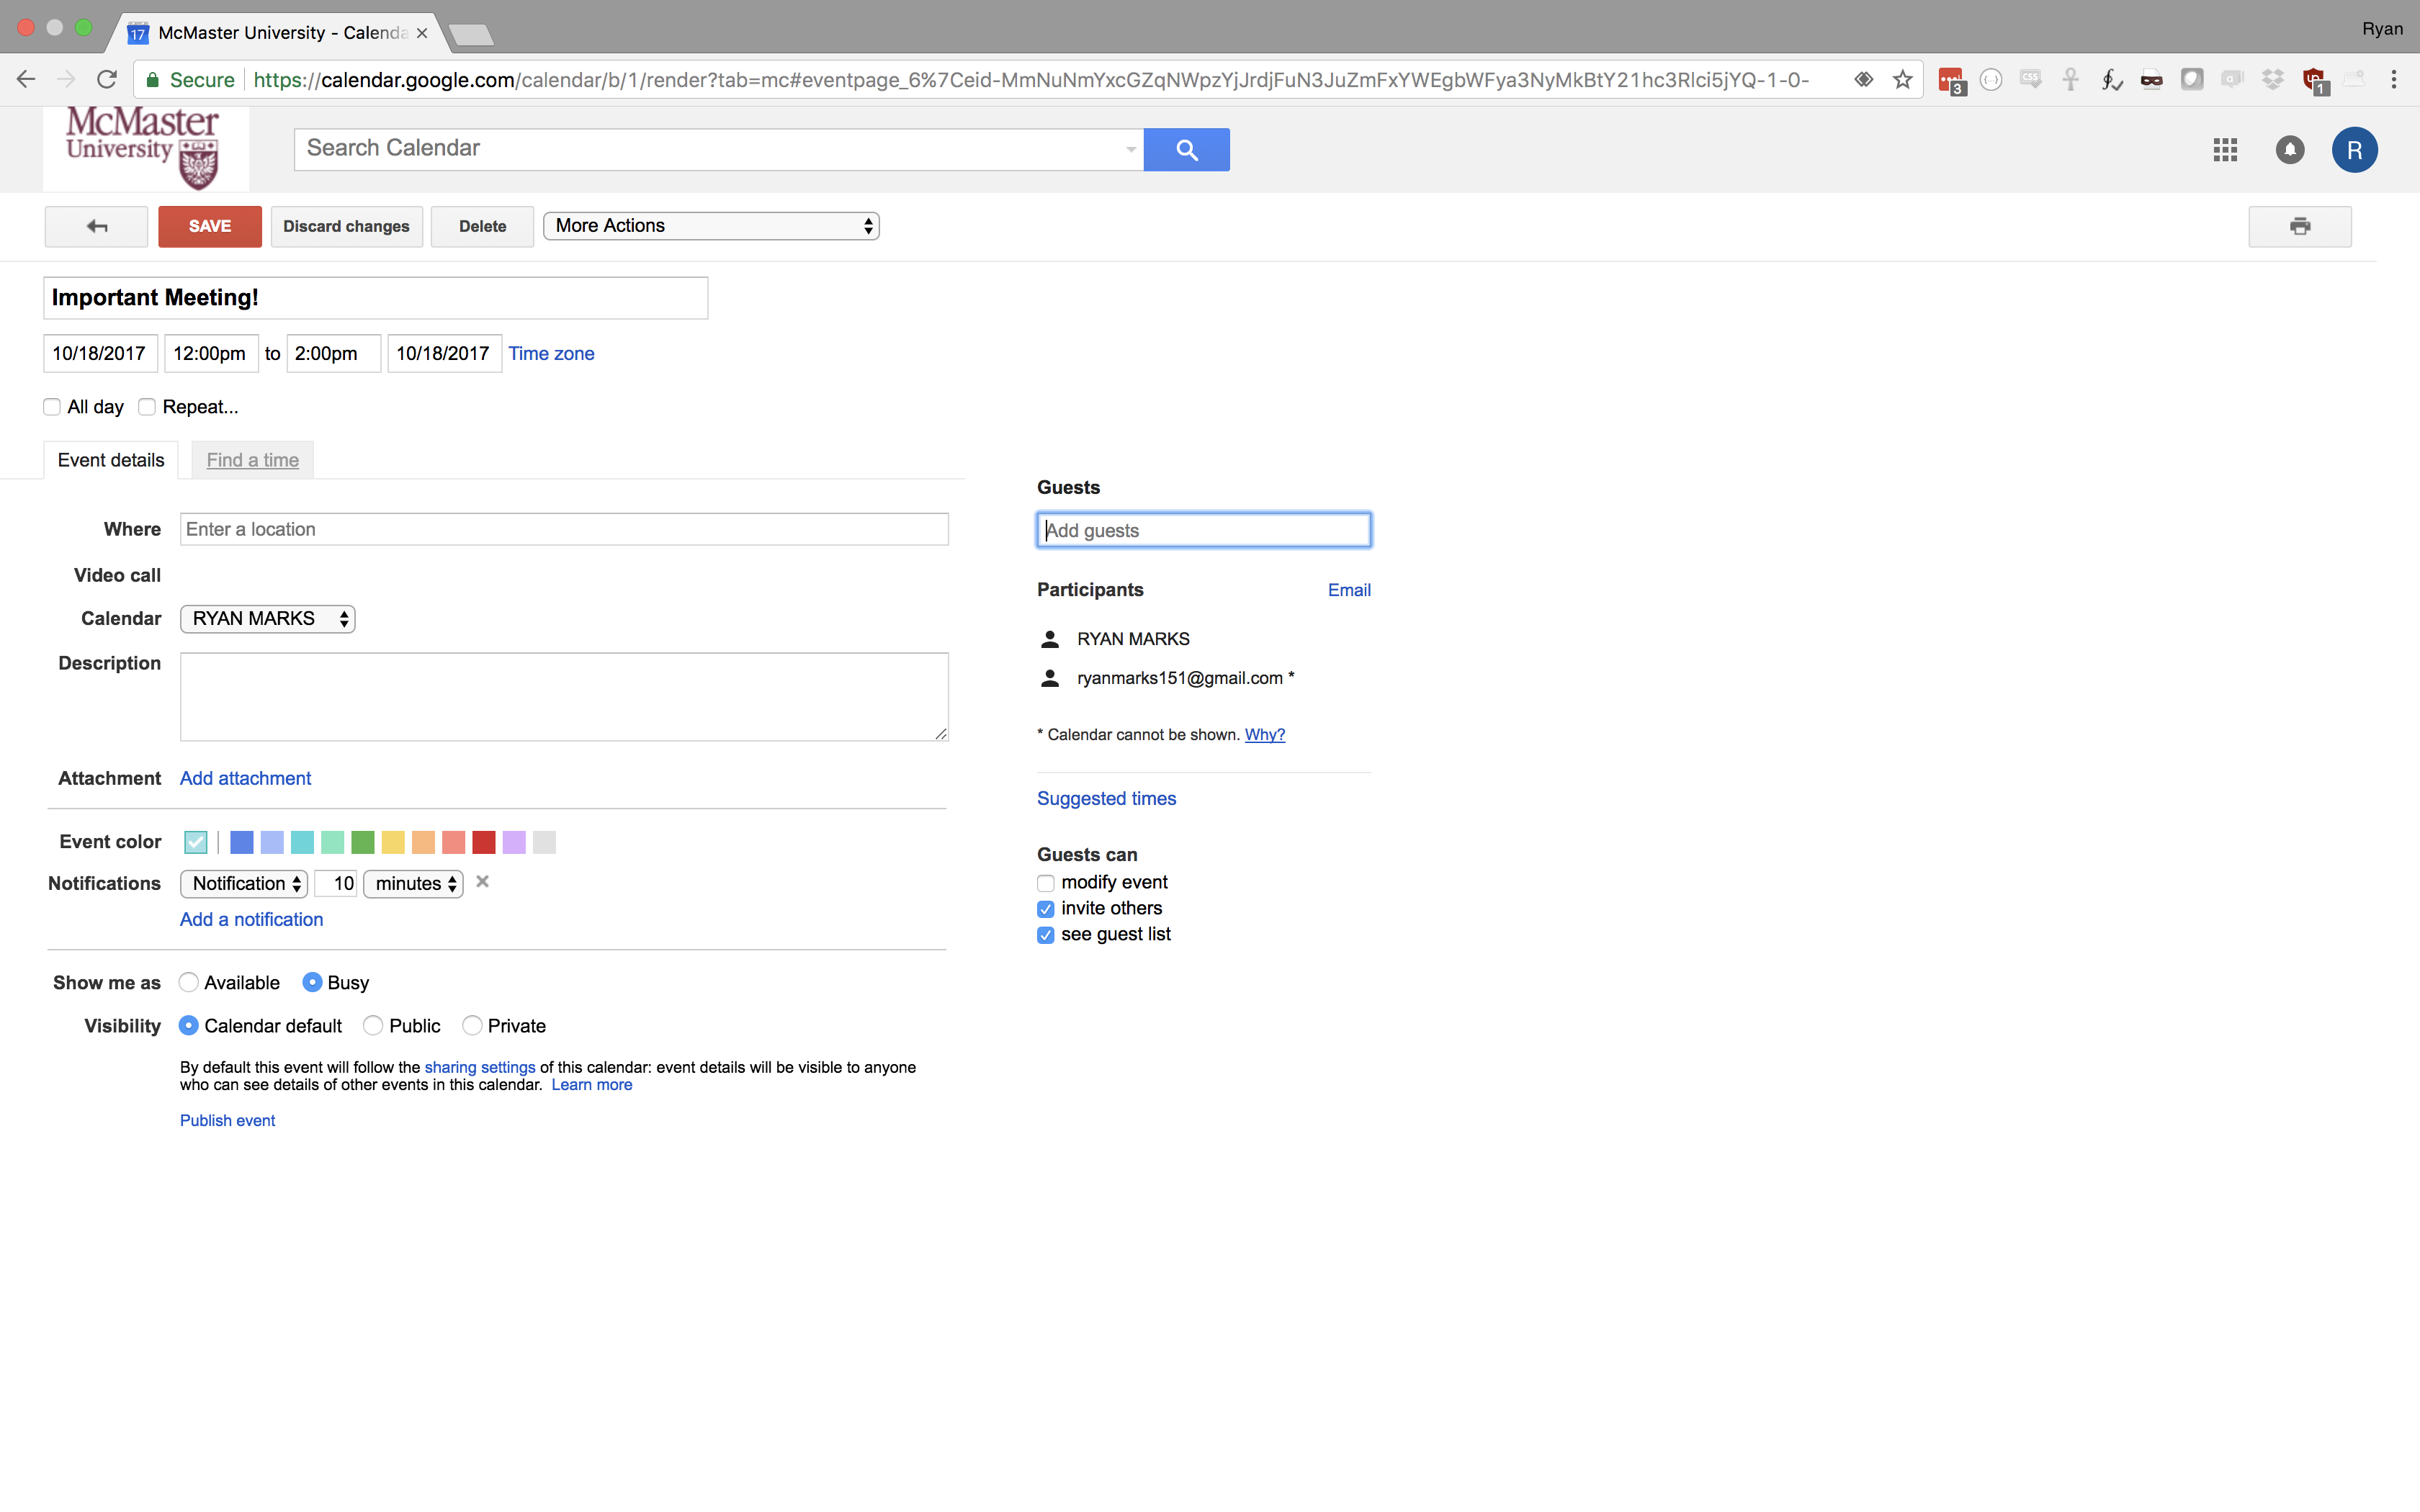
\includegraphics[width=\columnwidth]{{google/Invite2_2.png}}
\caption{Before subtask 2.2 of the invitation procedure for Google Calendar}
\end{figure}

\begin{figure}[H]
\centering
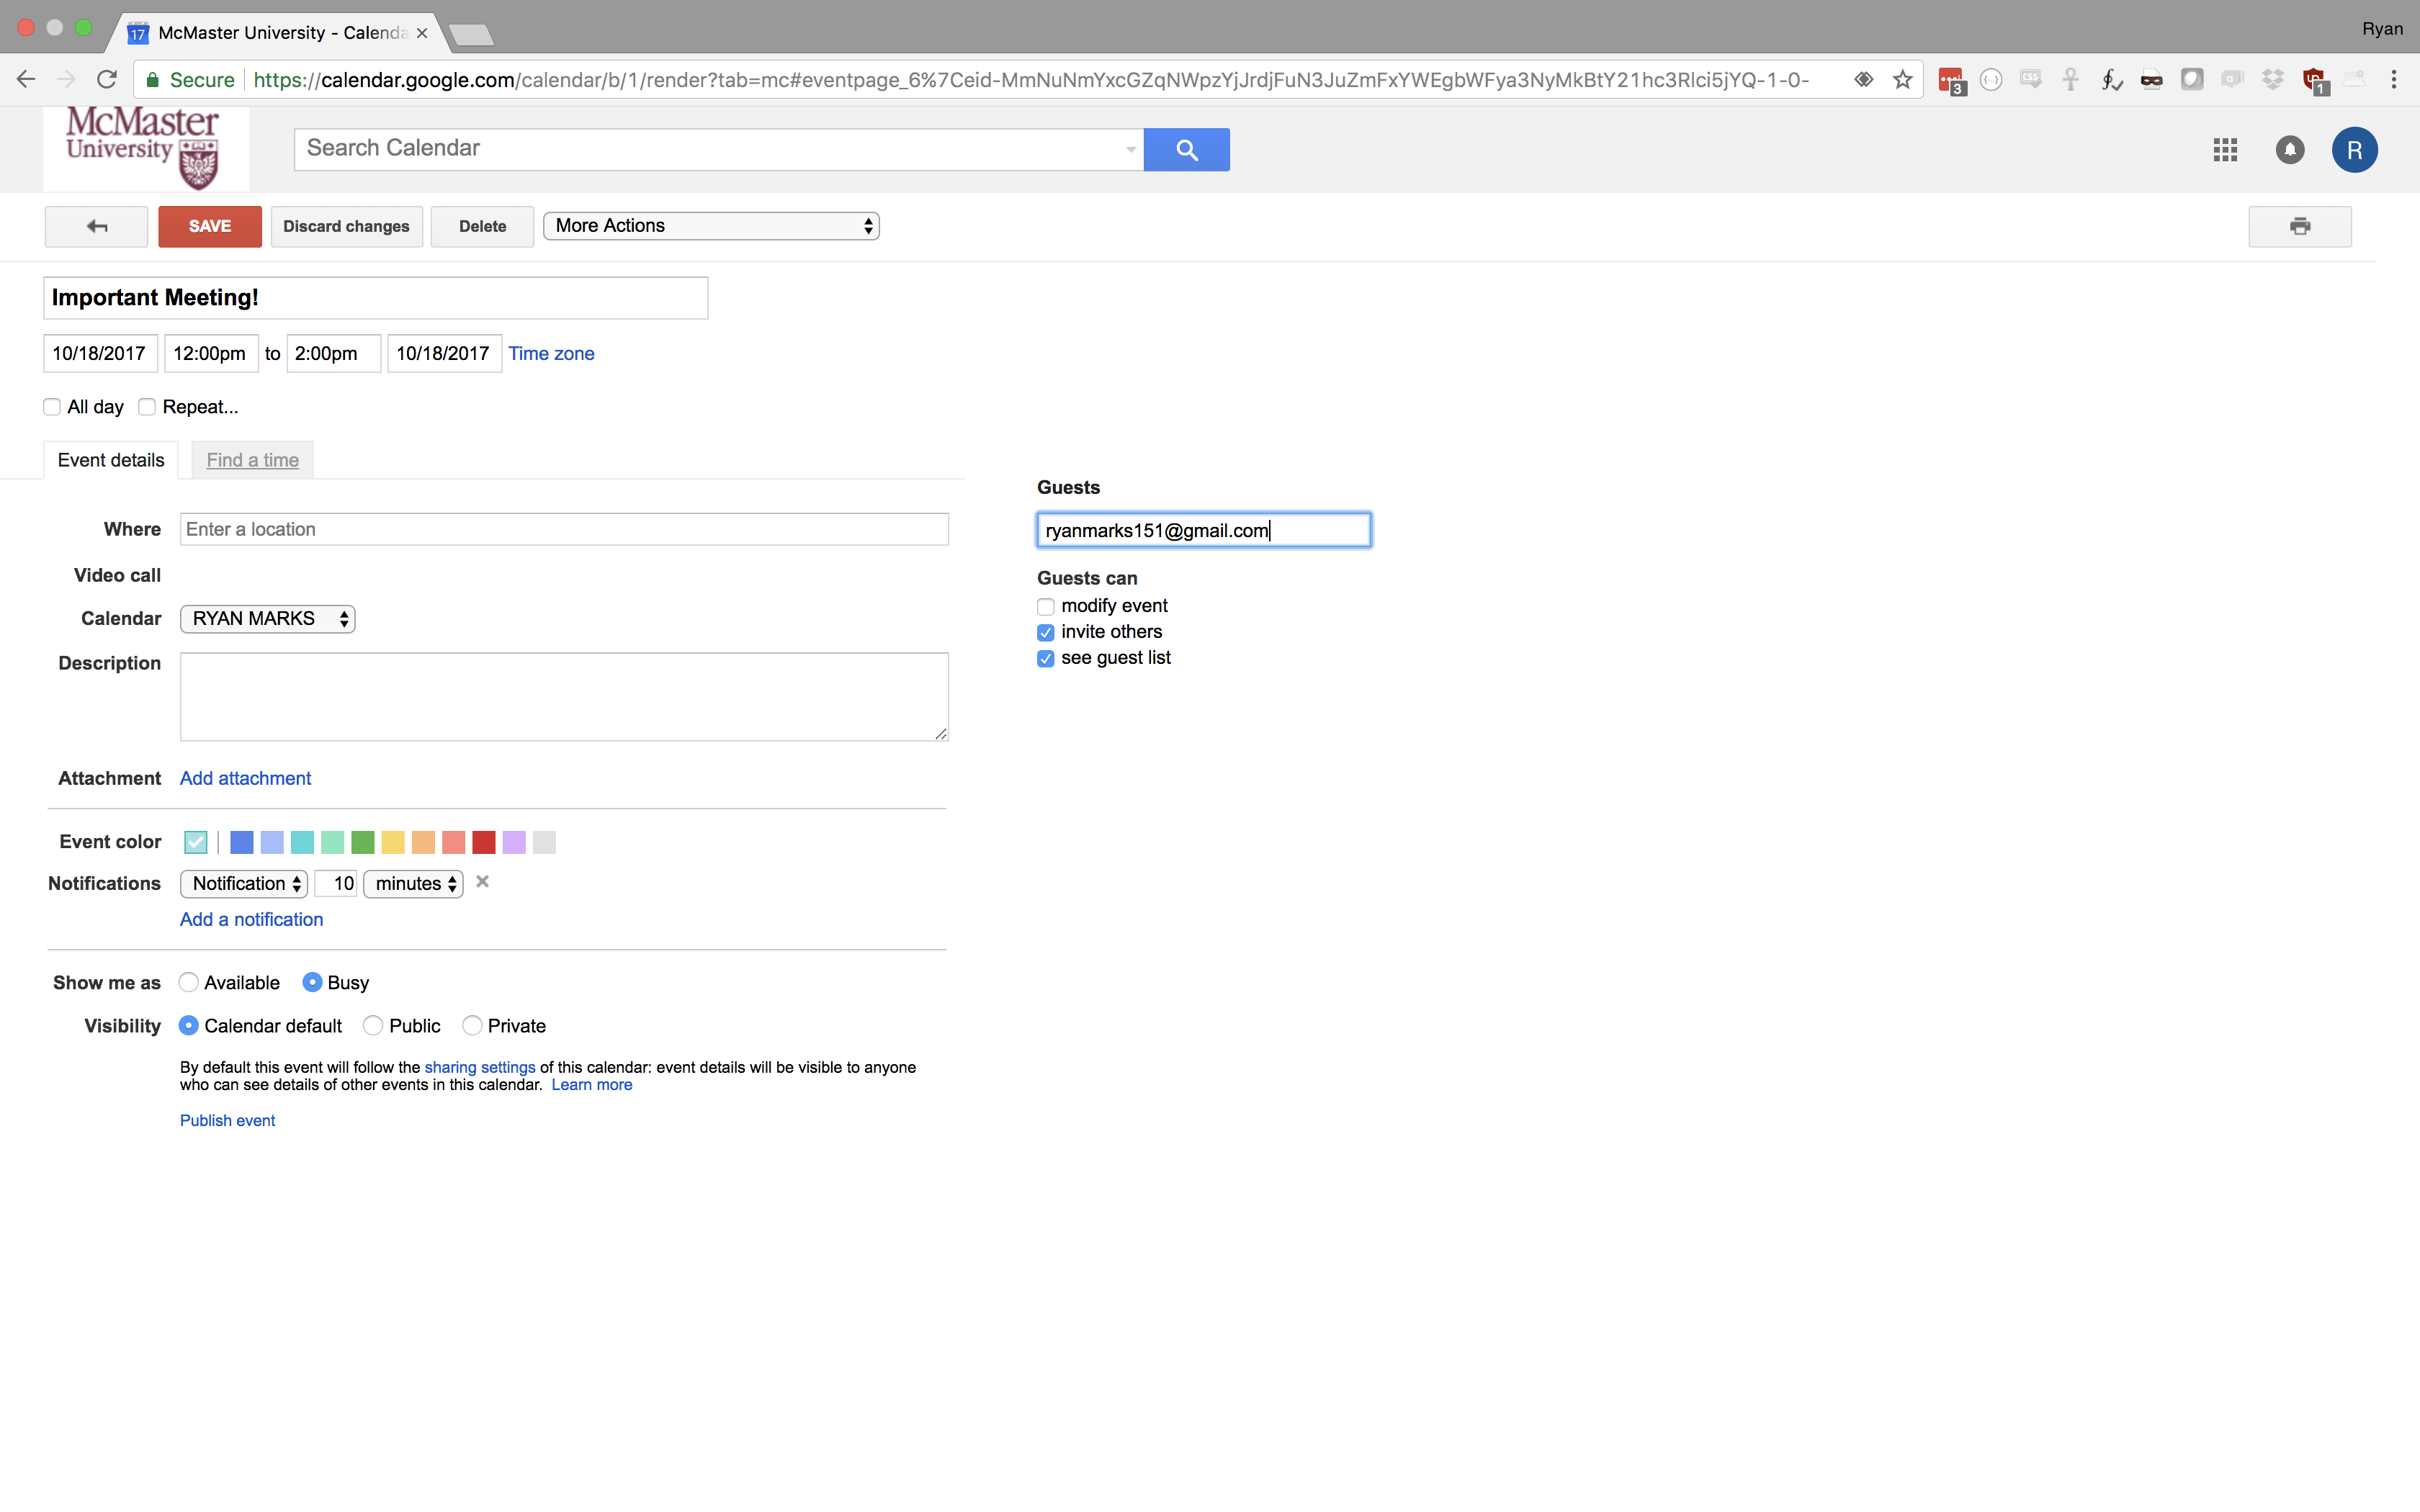
\includegraphics[width=\columnwidth]{{google/Invite2_2end.png}}
\caption{After subtask 2.2 of the invitation procedure for Google Calendar}
\end{figure}

\newpage

\begin{figure}[H]
\centering
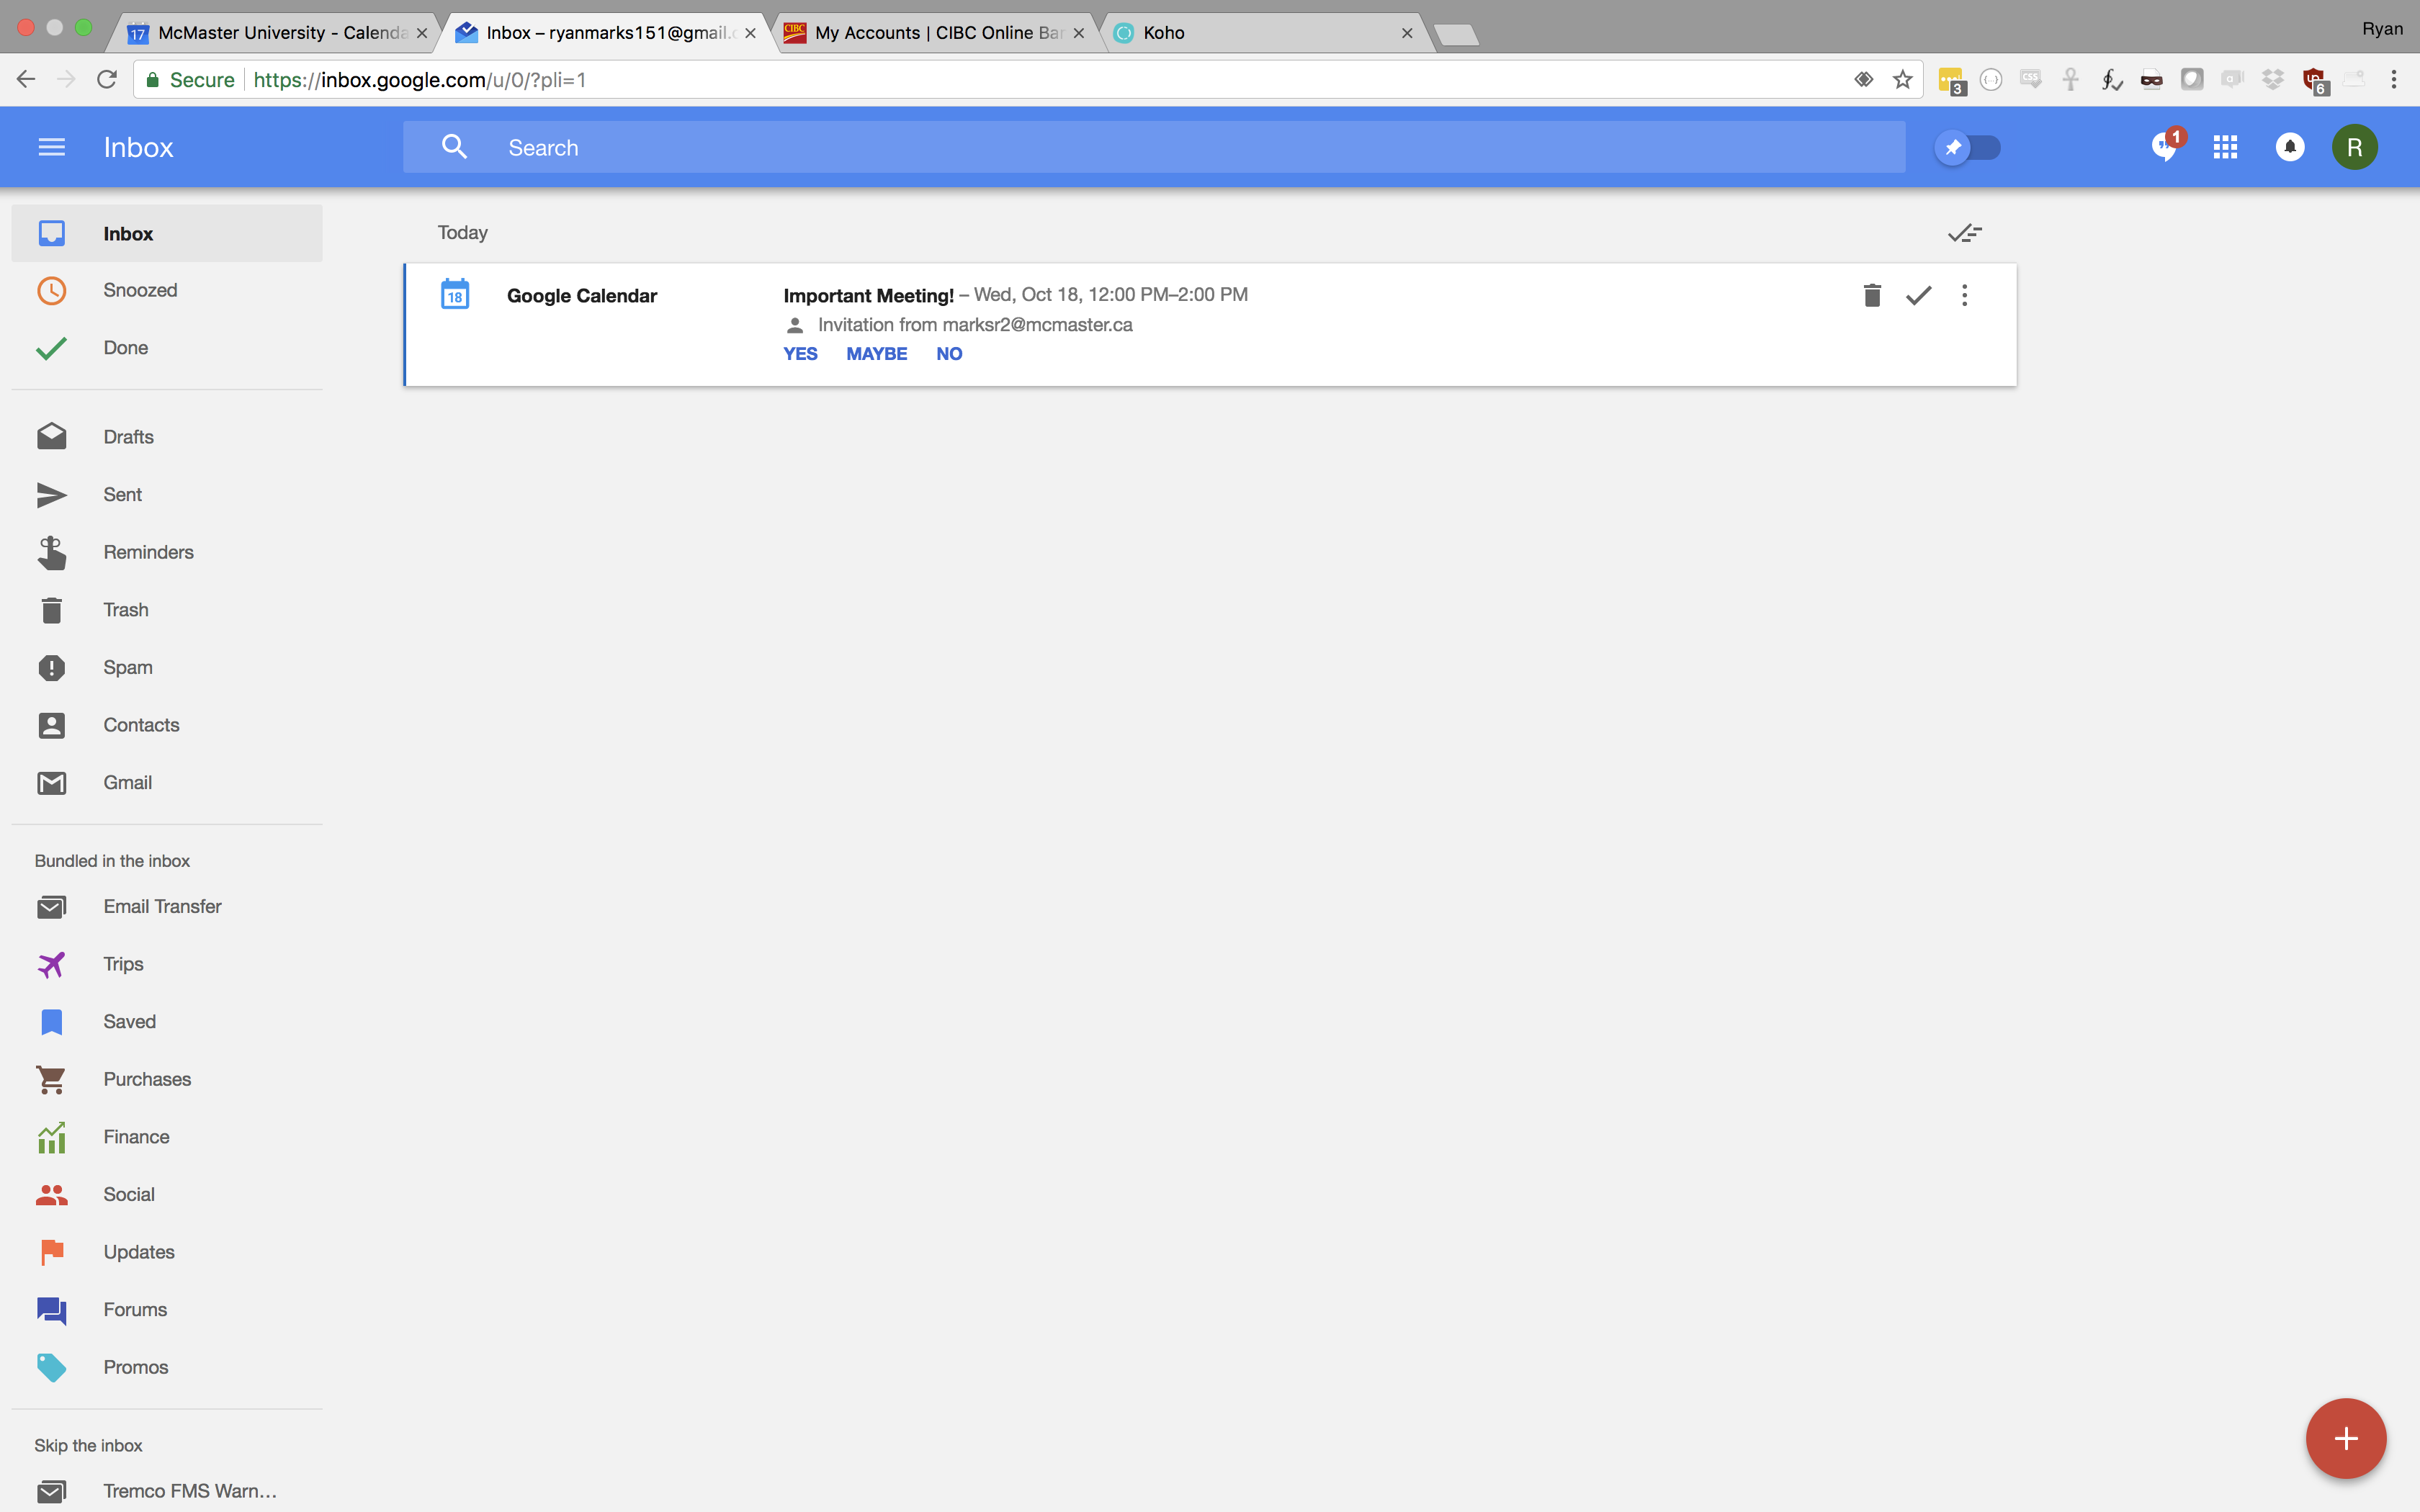
\includegraphics[width=\columnwidth]{{google/Respond1.png}}
\caption{Before subtask 1 of the invite response task with Google Inbox}
\end{figure}

\begin{figure}[H]
\centering
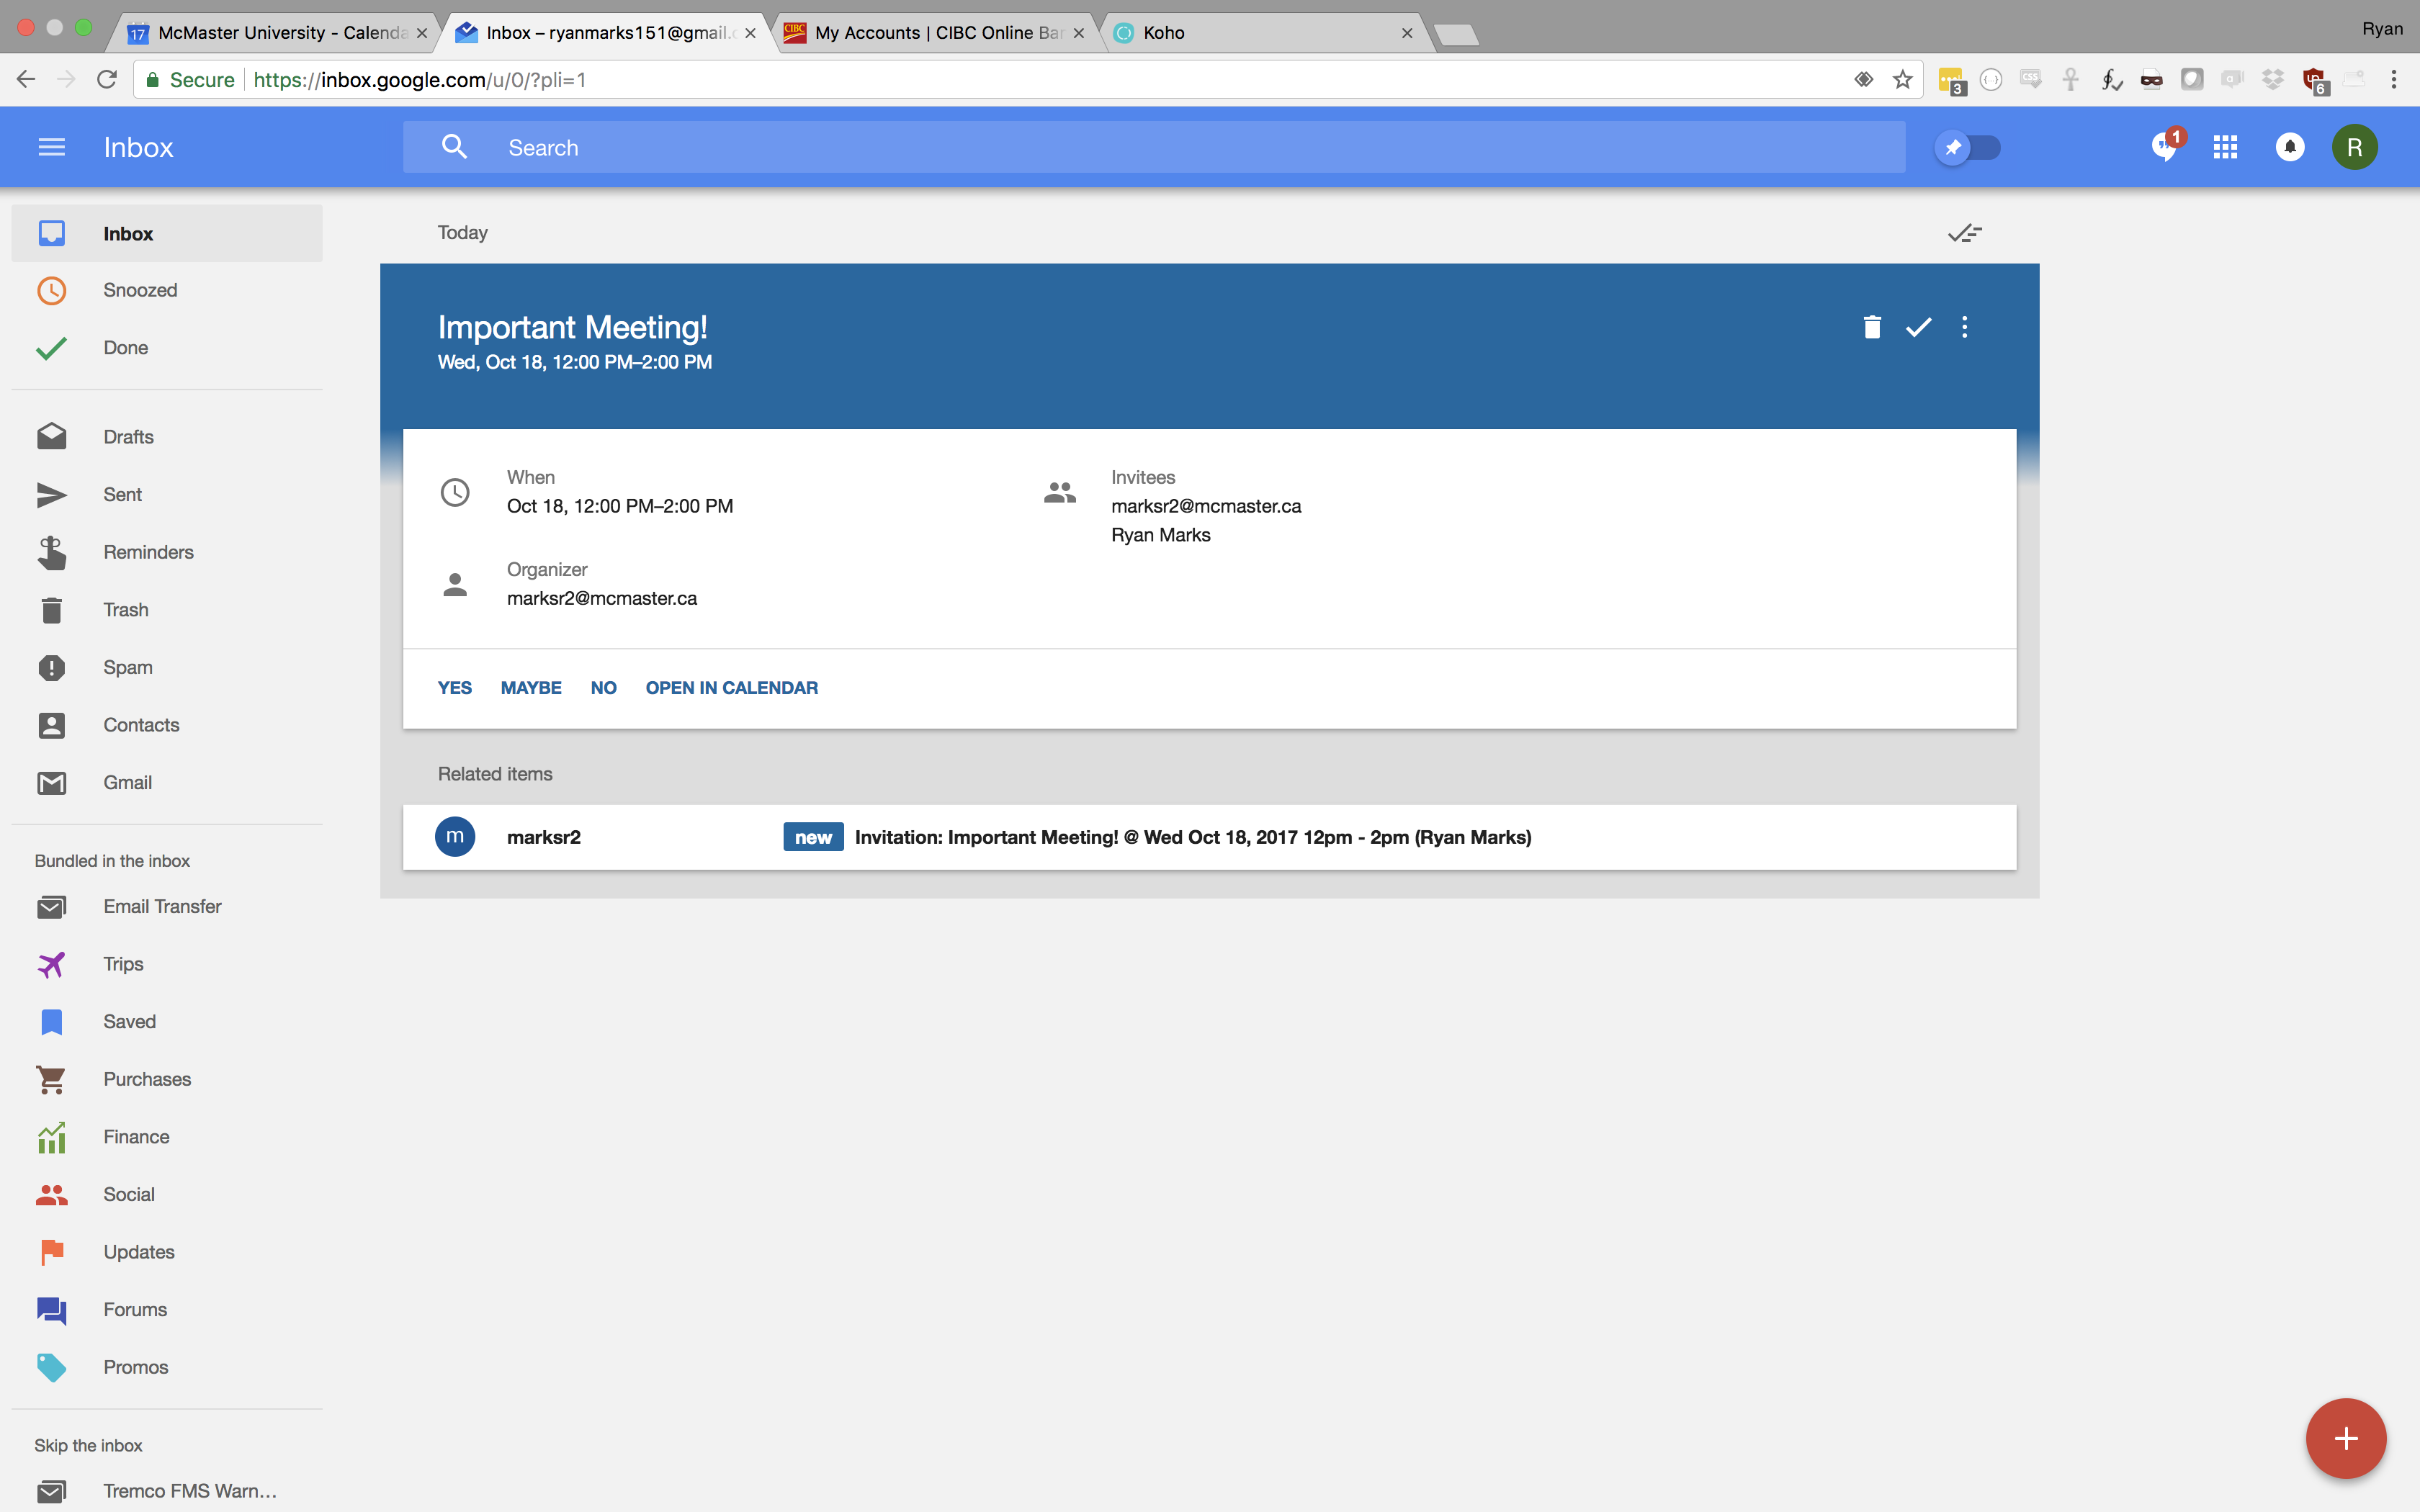
\includegraphics[width=\columnwidth]{{google/Respond1end.png}}
\caption{After subtask 1 of the invite response task with Google Inbox}
\end{figure}

\begin{figure}[H]
\centering
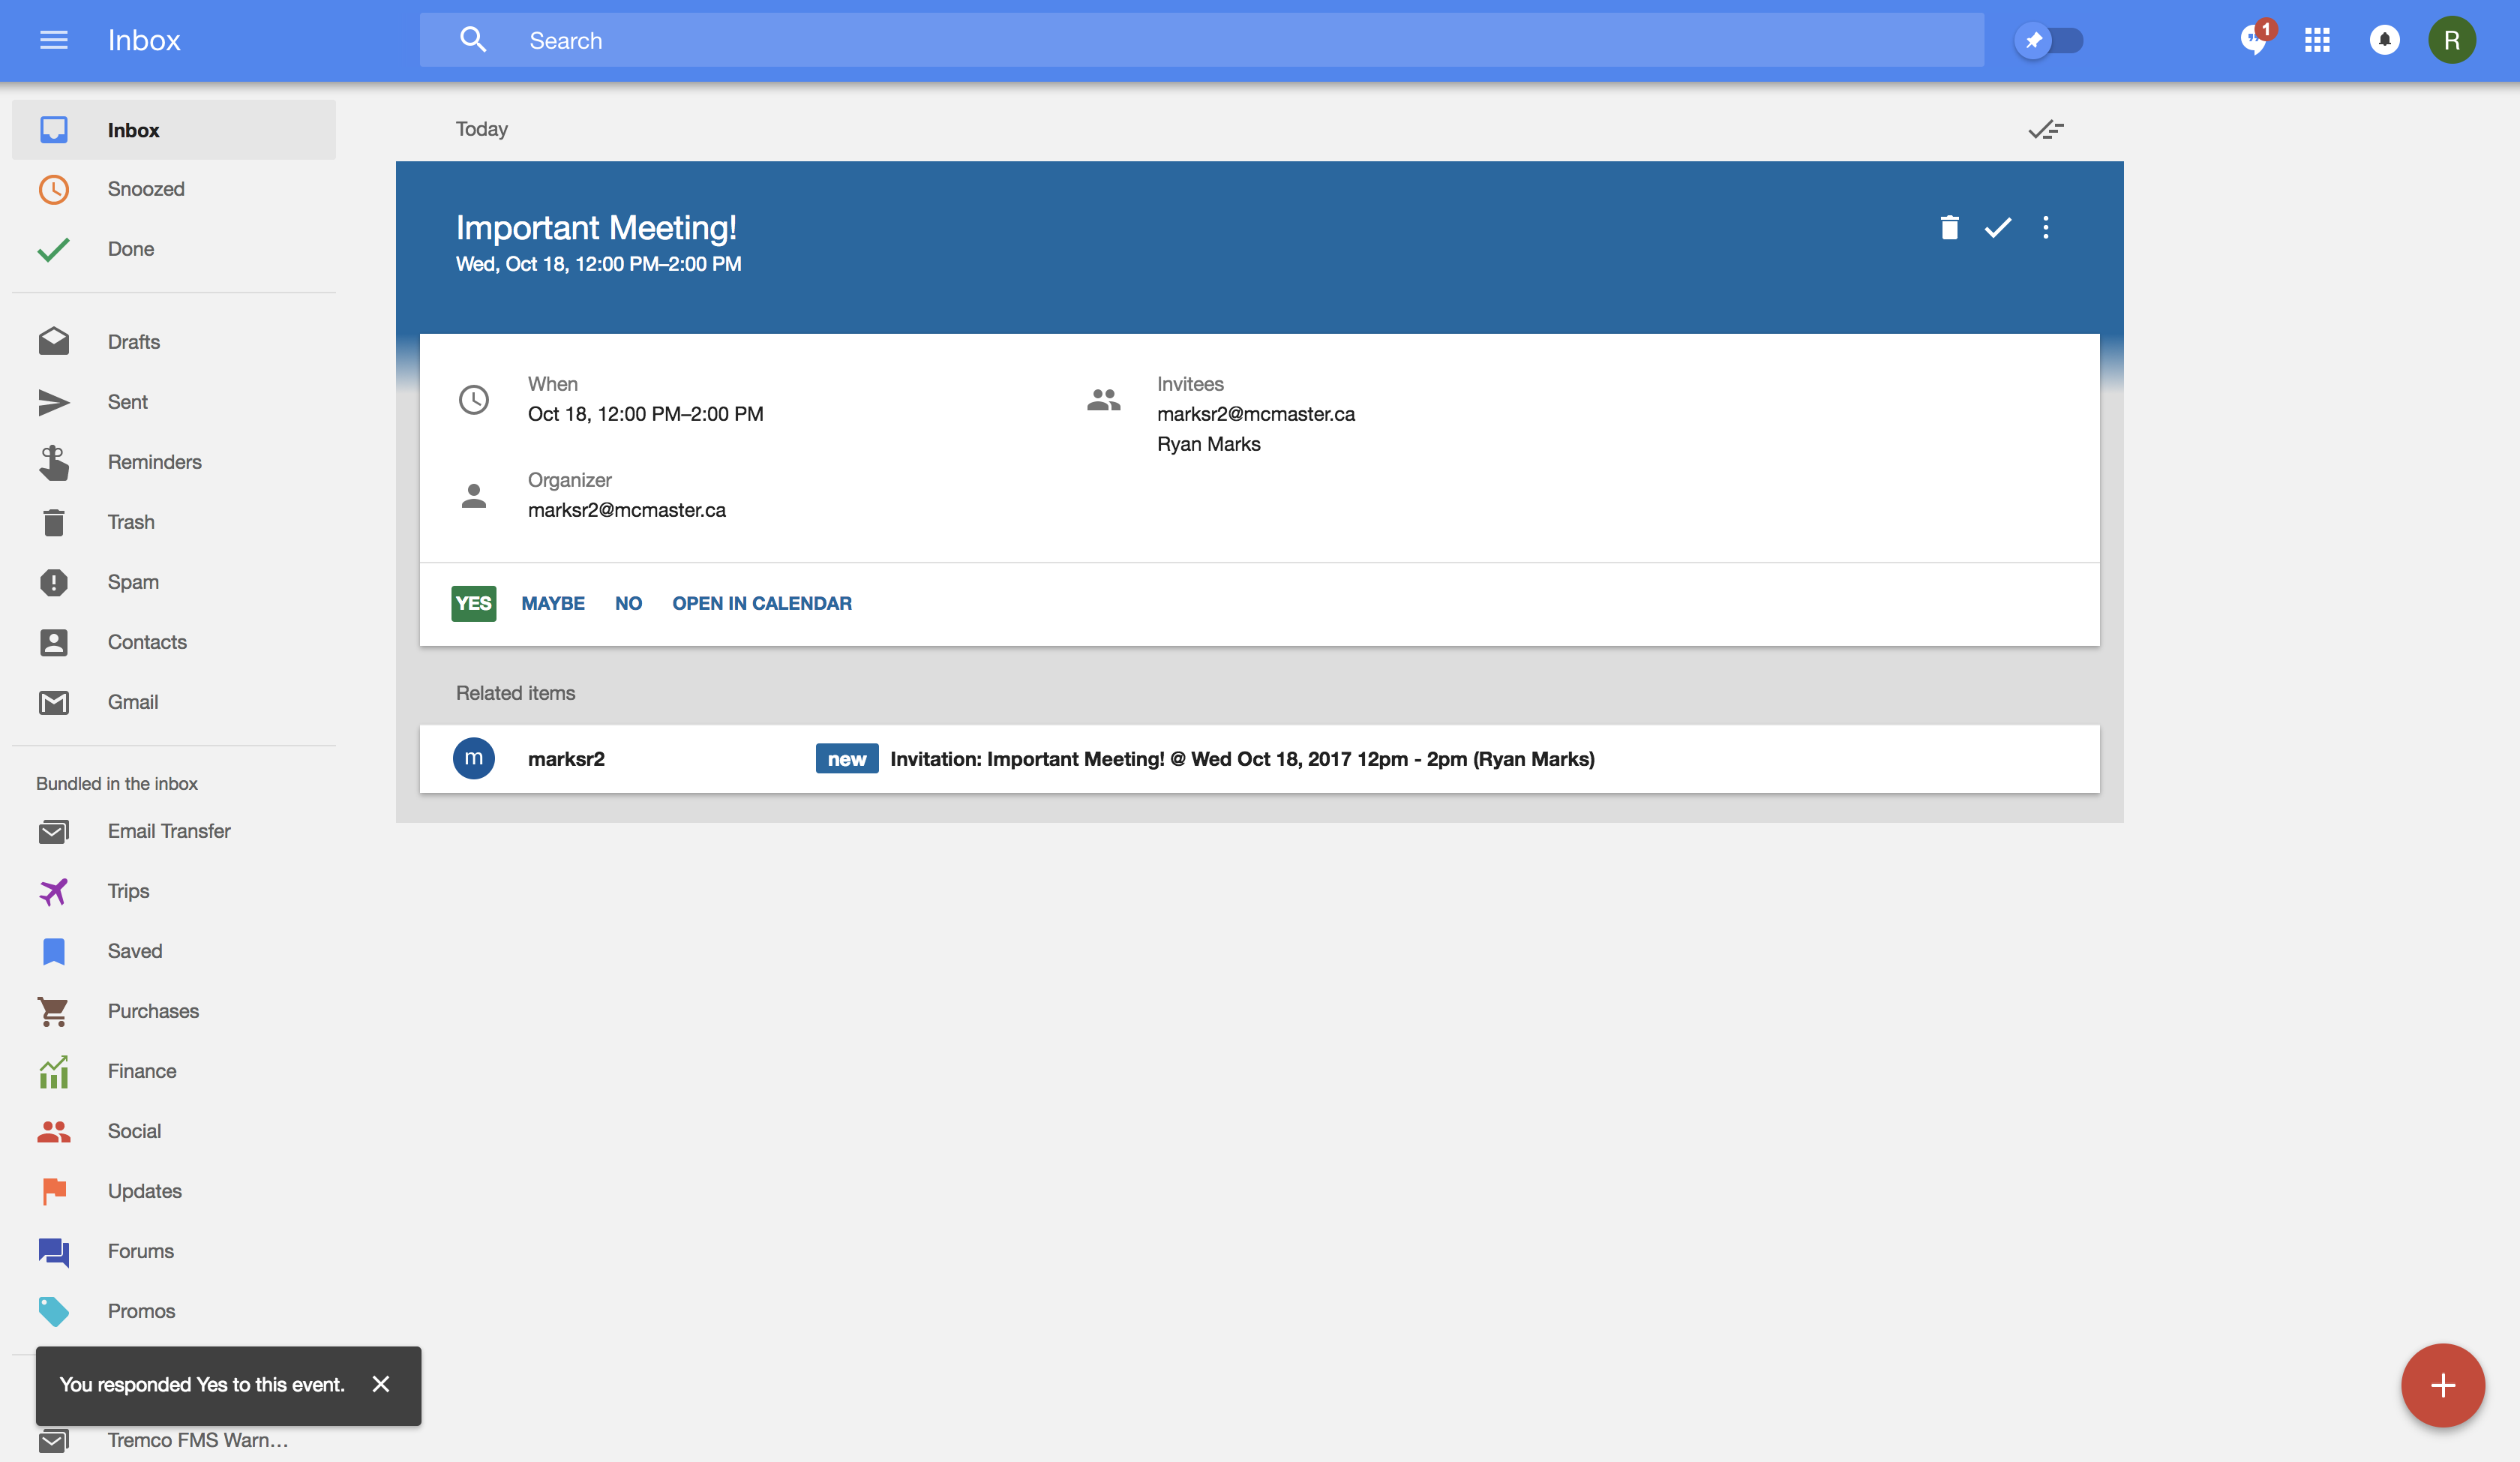
\includegraphics[width=\columnwidth]{{google/Respond2_1.png}}
\caption{Subtask 2.1 of the invite response task with Google Inbox}
\end{figure}


\begin{figure}[H]
\centering
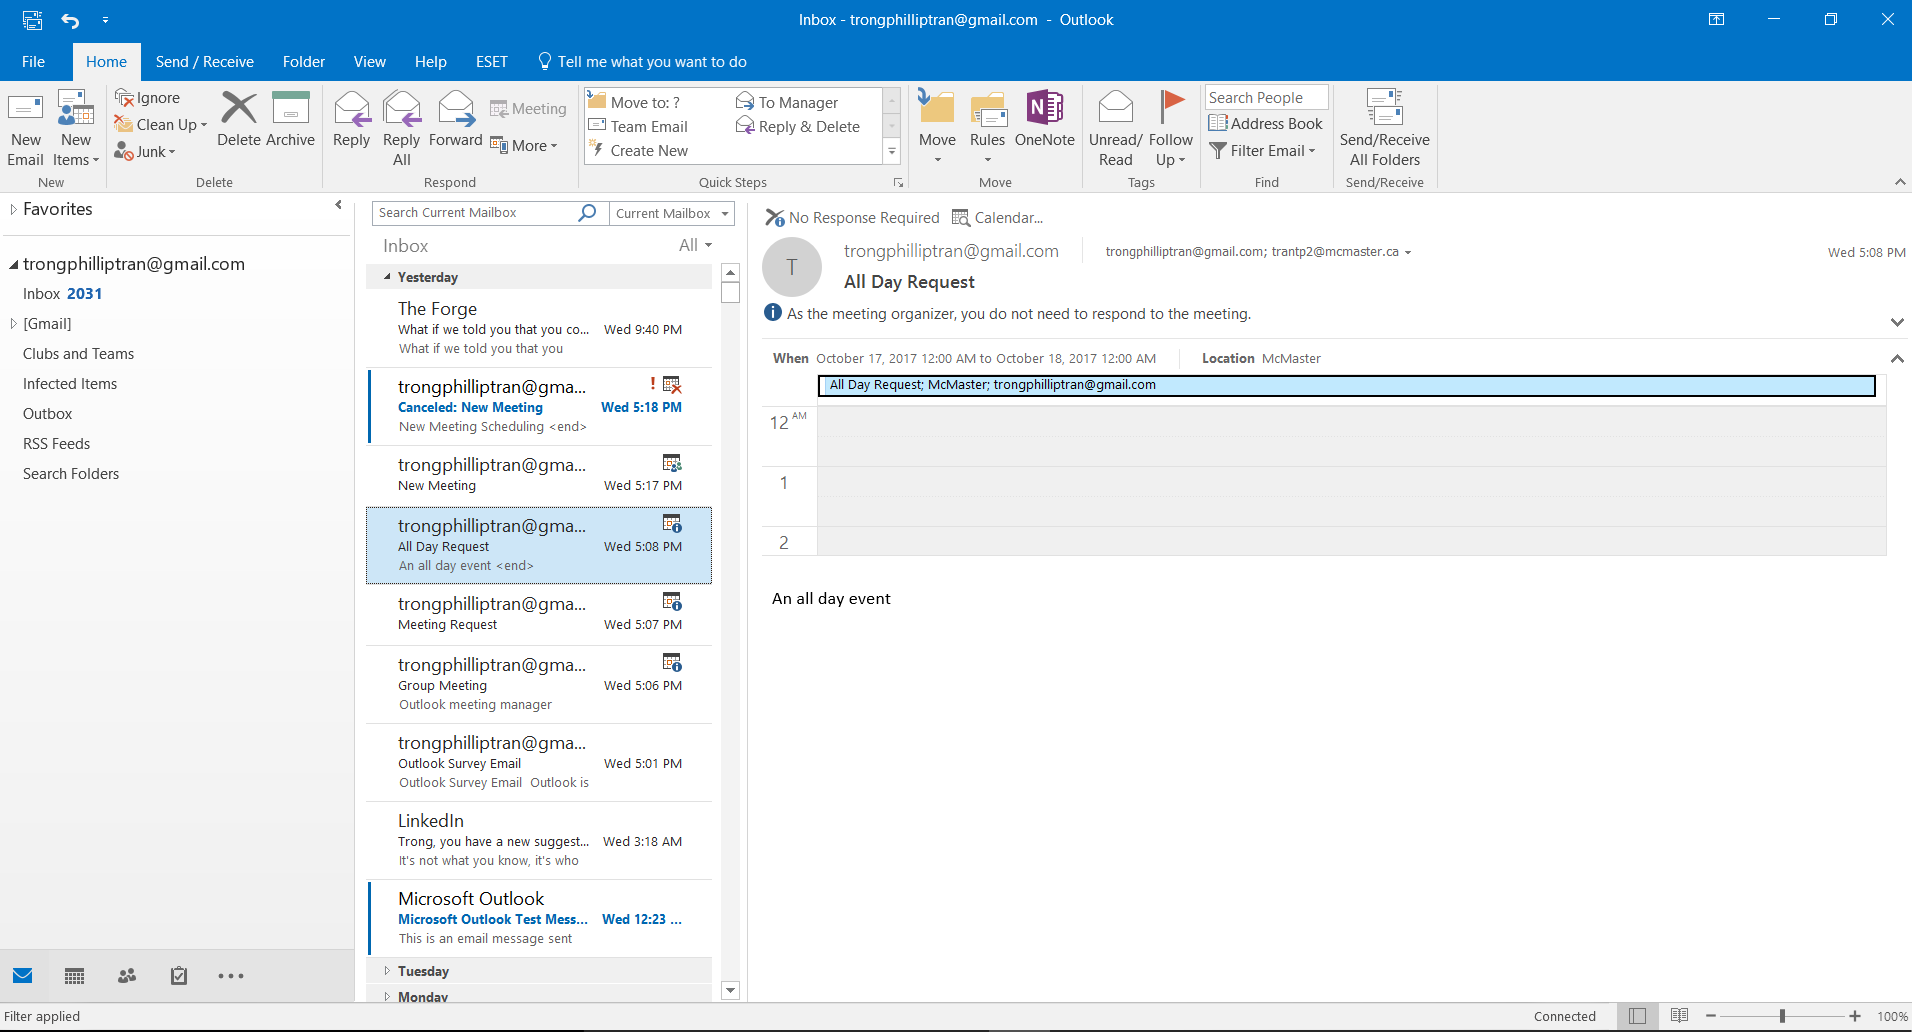
\includegraphics[width=\columnwidth]{{Outlook/Critique_Picture.png}}
\caption{Outlook has many options, which can be overwhelming if a user has no experience in using Microsoft Office type applications}
\end{figure}

\begin{figure}[H]
\centering
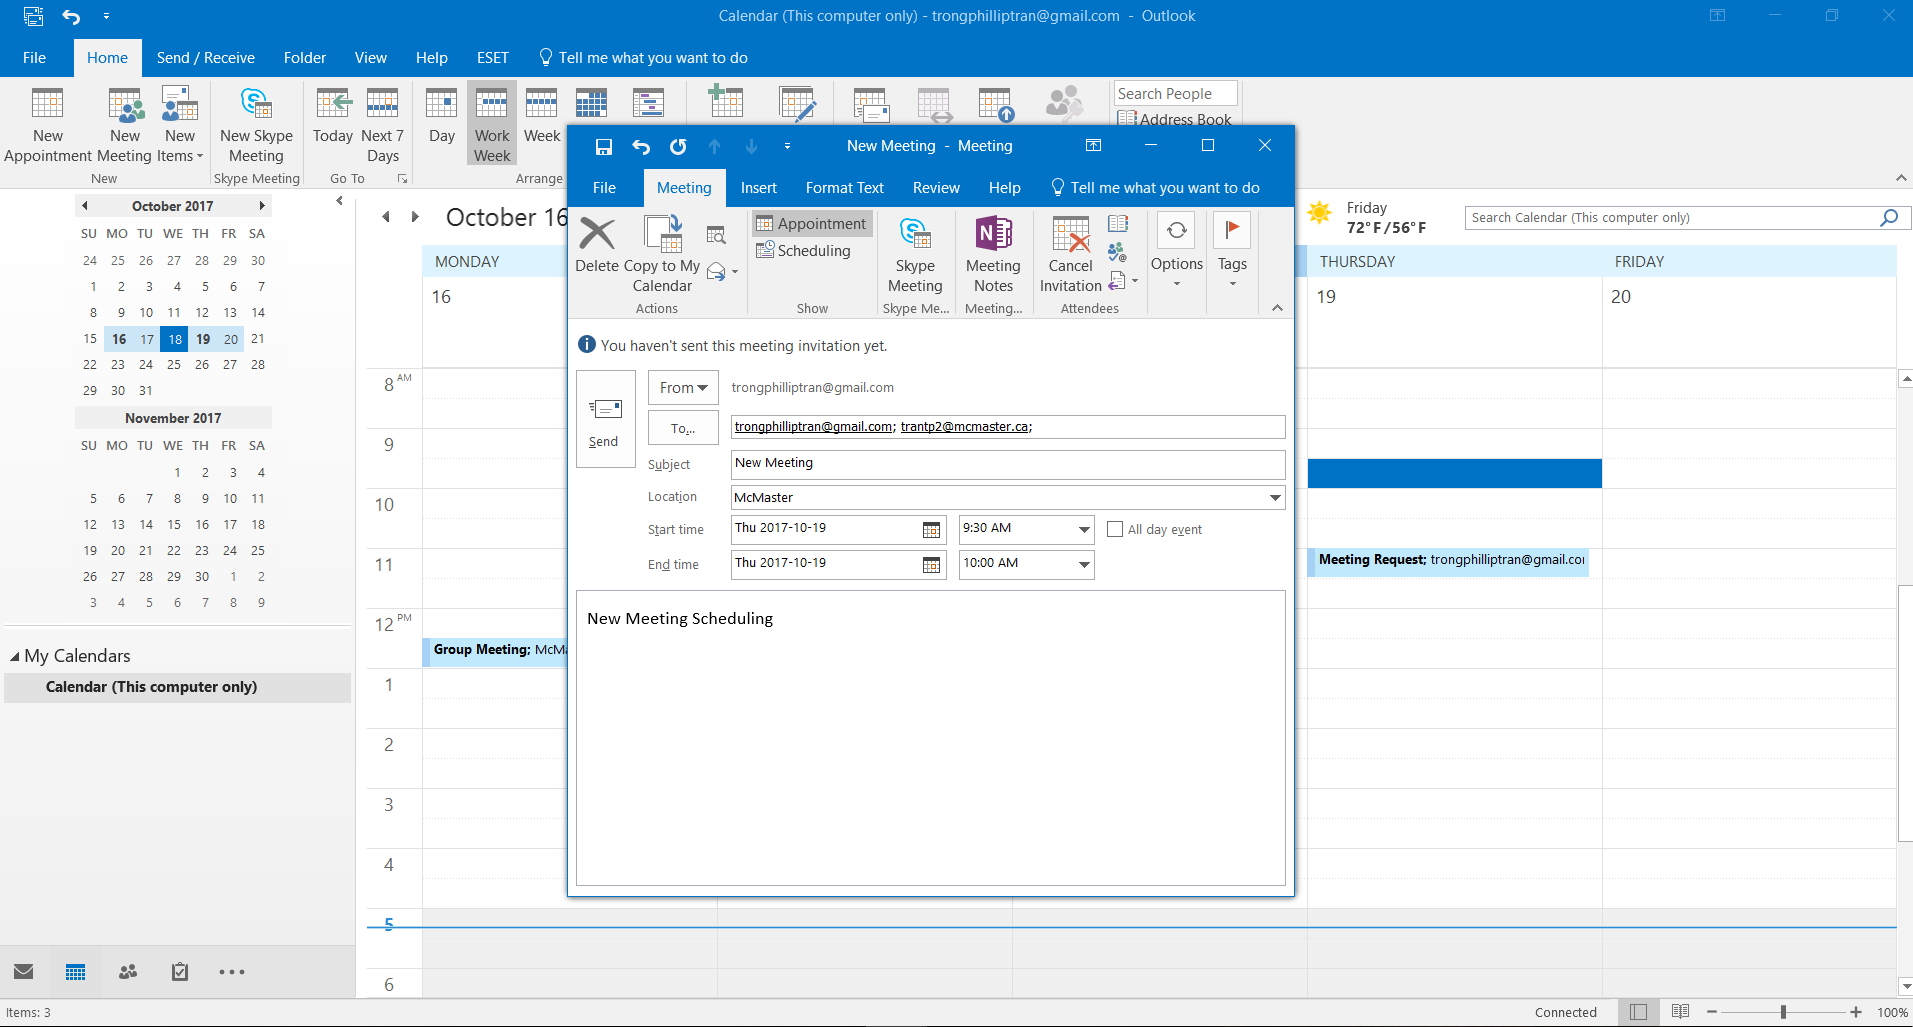
\includegraphics[width=\columnwidth]{{Outlook/New_Meeting_Schedule.png}}
\caption{New Meeting Scheduling}
\end{figure}

\begin{figure}[H]
\centering
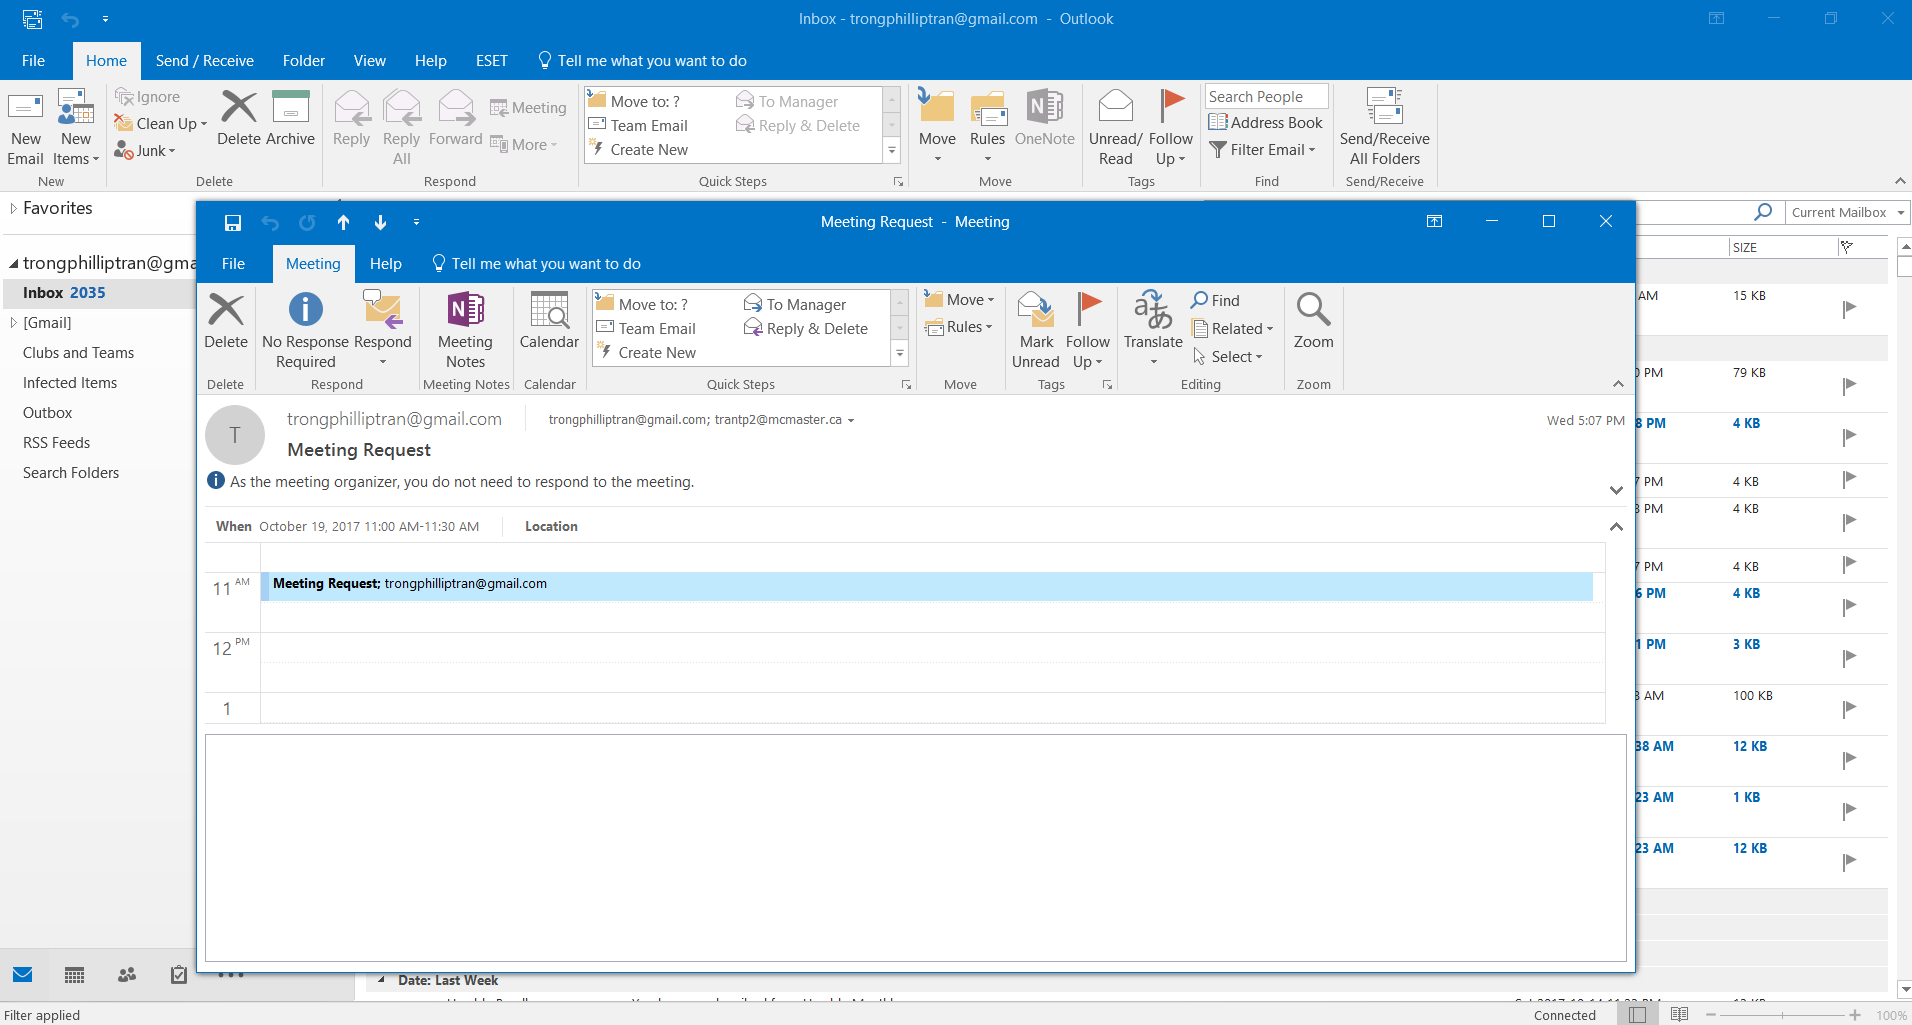
\includegraphics[width=\columnwidth]{{Outlook/Meeting_Request_Response.png}}
\caption{Meeting Request Response}
\end{figure}

\begin{figure}[H]
\centering
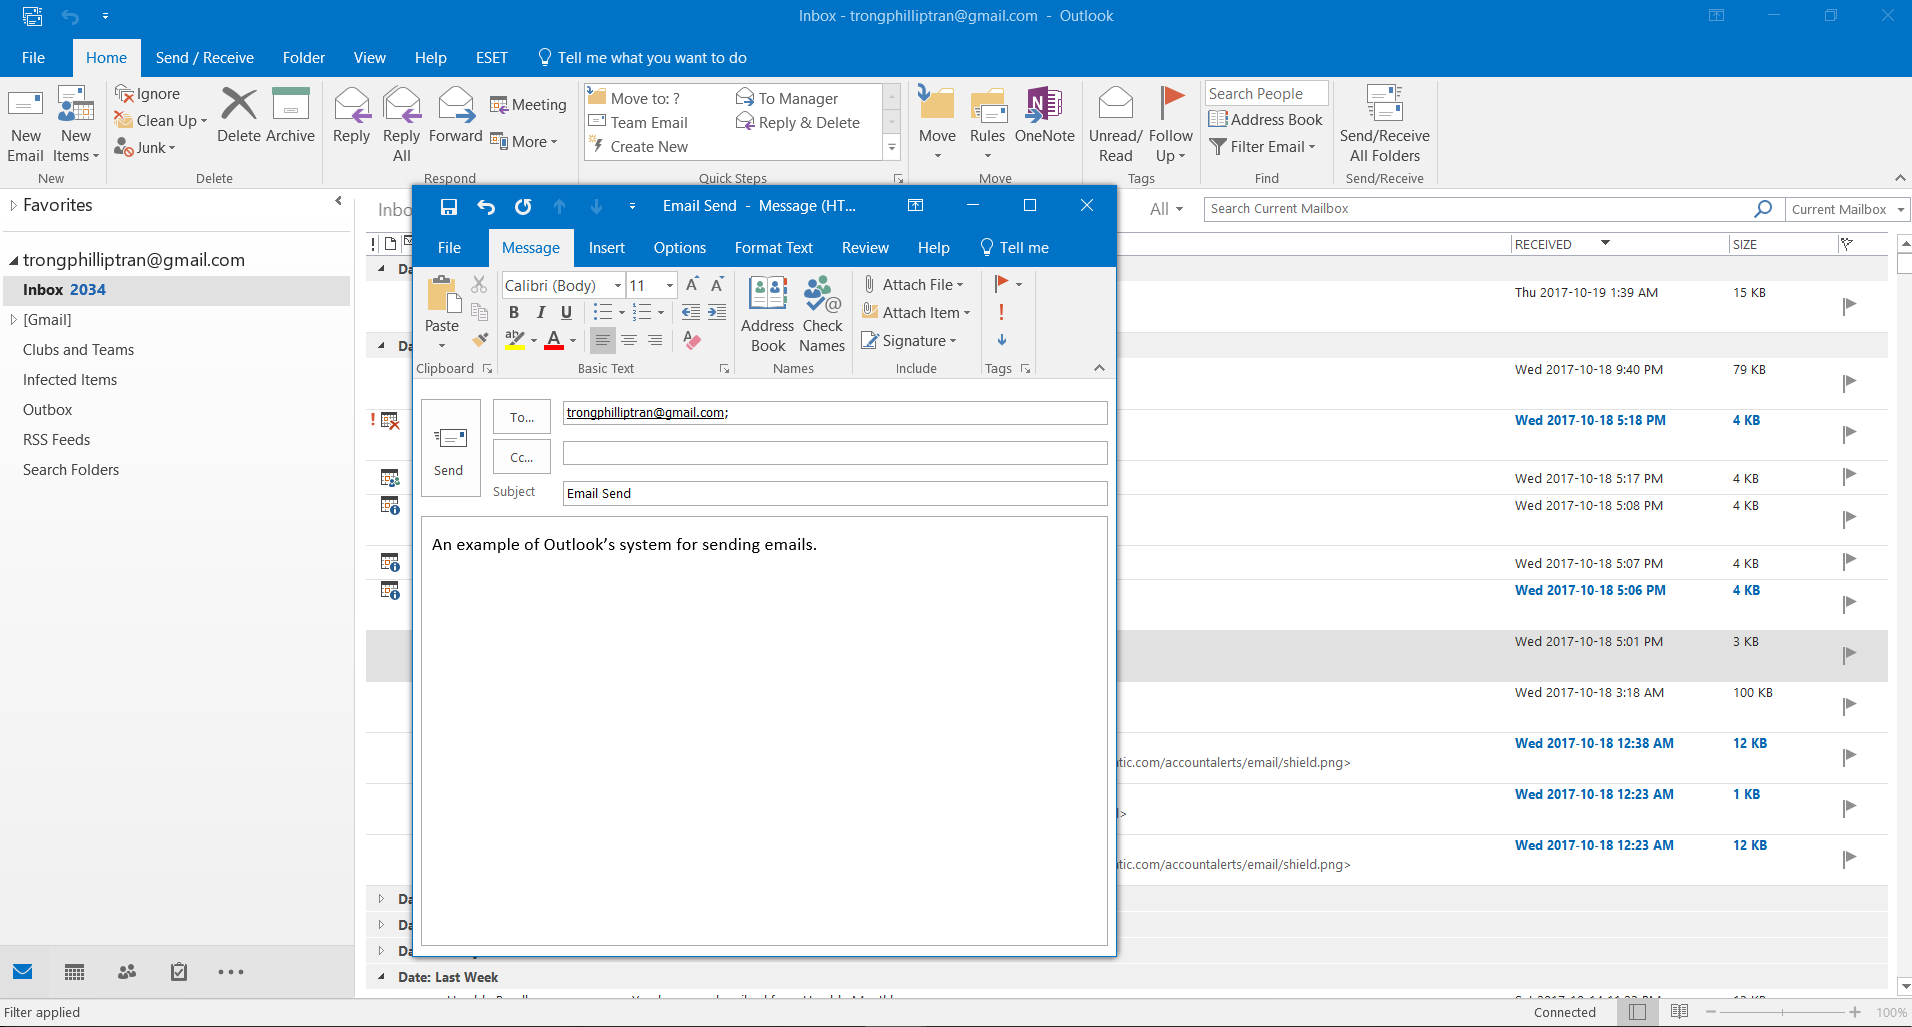
\includegraphics[width=\columnwidth]{{Outlook/Email_Send.png}}
\caption{Meeting Request Response}
\end{figure}

\begin{figure}[H]
\centering
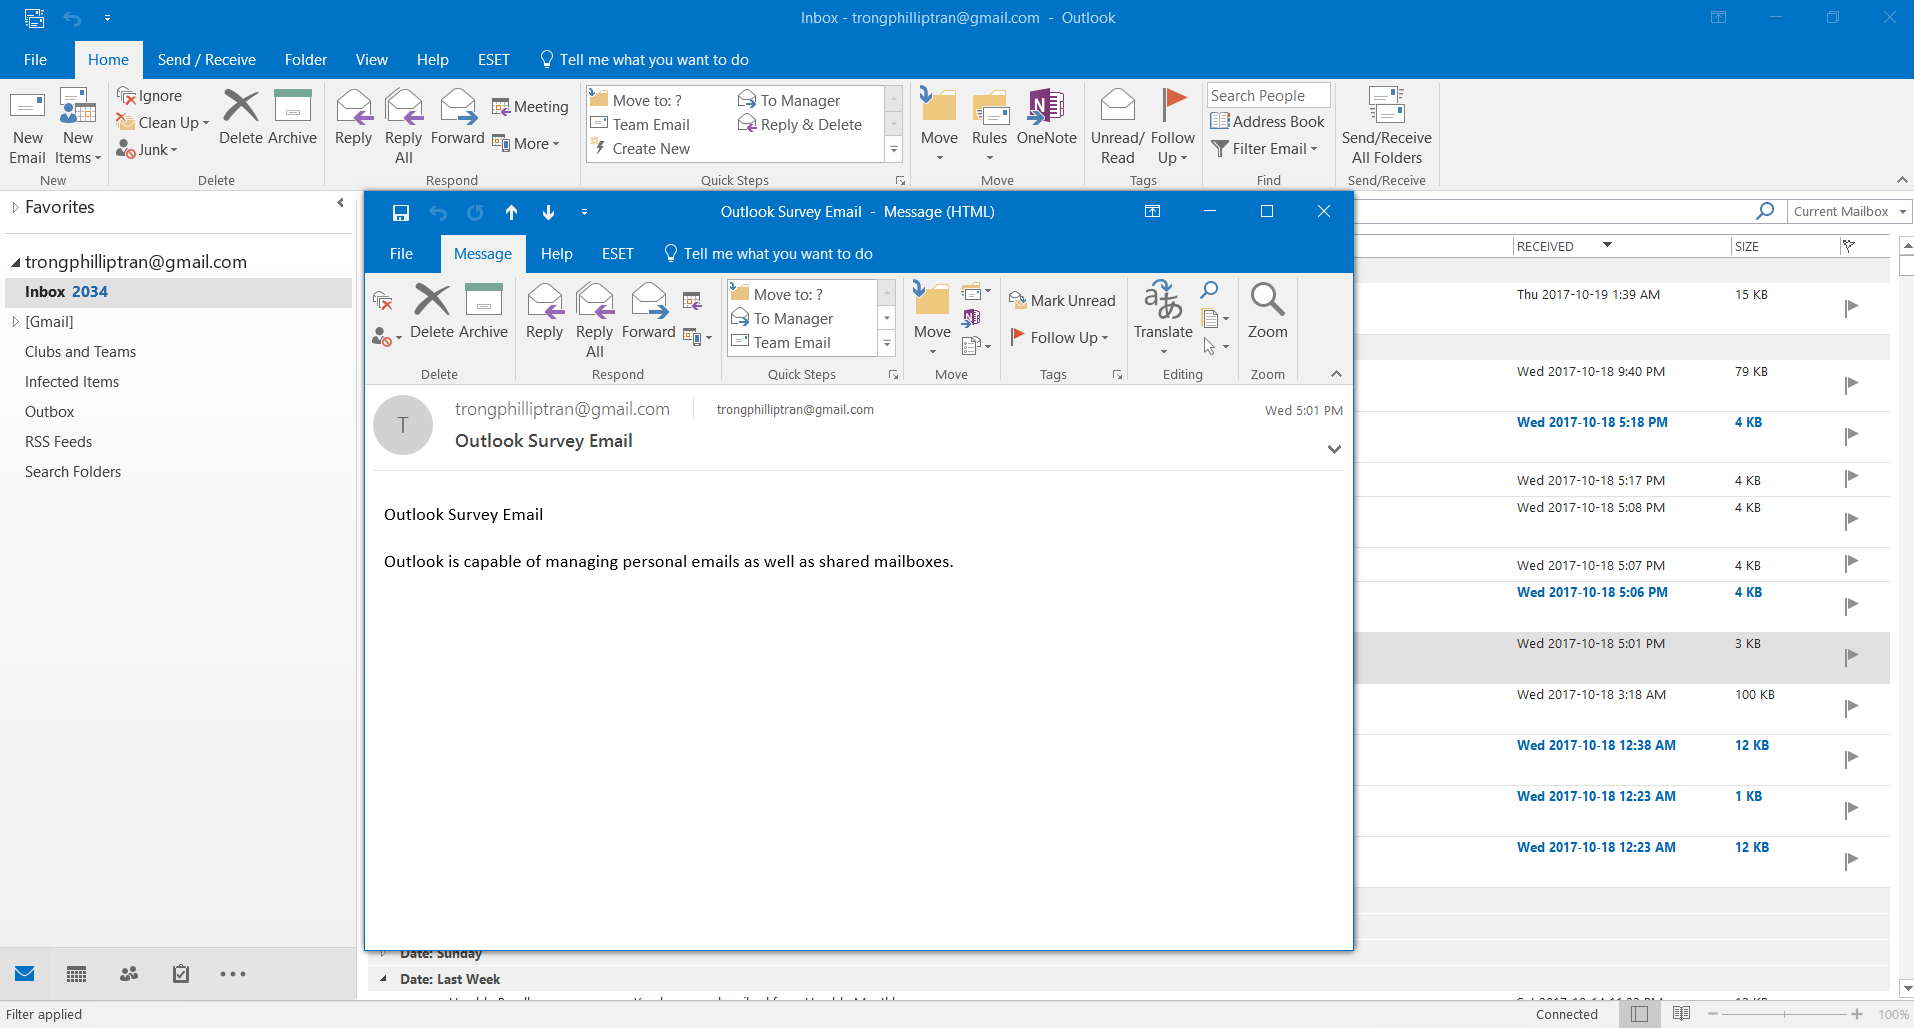
\includegraphics[width=\columnwidth]{{Outlook/Email_Reply.png}}
\caption{Meeting Request Response}
\end{figure}


\end{document}

%%% Local Variables:
%%% mode: latex
%%% TeX-master: t
%%% End:
